\input{"preamble.tex"}

\addbibresource{UGA\_Real\_Analysis\_Qual\_Solutions.bib}

\let\Begin\begin
\let\End\end
\newcommand\wrapenv[1]{#1}

\makeatletter
\def\ScaleWidthIfNeeded{%
 \ifdim\Gin@nat@width>\linewidth
    \linewidth
  \else
    \Gin@nat@width
  \fi
}
\def\ScaleHeightIfNeeded{%
  \ifdim\Gin@nat@height>0.9\textheight
    0.9\textheight
  \else
    \Gin@nat@width
  \fi
}
\makeatother

\setkeys{Gin}{width=\ScaleWidthIfNeeded,height=\ScaleHeightIfNeeded,keepaspectratio}%

\title{
\textbf{
    UGA Real Analysis Solutions (Fall 2014 -- Spring 2021)
  }
  }







\begin{document}

\date{}
\maketitle


\newpage

% Note: addsec only in KomaScript
\addsec{Table of Contents}
\tableofcontents
\newpage

\hypertarget{preface}{%
\section{Preface}\label{preface}}

I'd like to extend my gratitude to Peter Woolfitt for supplying many
solutions and checking many proofs of the rest in problem sessions. Many
other solutions contain input and ideas from other graduate students and
faculty members at UGA, along with questions and answers posted on Math
Stack Exchange or Math Overflow.

\hypertarget{undergraduate-analysis-uniform-convergence}{%
\section{Undergraduate Analysis: Uniform
Convergence}\label{undergraduate-analysis-uniform-convergence}}

\hypertarget{fall-2018-1-done}{%
\subsection{\texorpdfstring{Fall 2018 \# 1
\(\done\)}{Fall 2018 \# 1 \textbackslash done}}\label{fall-2018-1-done}}

Let \(f(x) = \frac 1 x\). Show that \(f\) is uniformly continuous on
\((1, \infty)\) but not on \((0,\infty)\).

\begin{concept}

\envlist

\begin{itemize}
\item
  Uniform continuity:
  \begin{align*}  
  \forall \varepsilon>0, \exists \delta({\varepsilon})>0 \quad\text{such that}\quad {\left\lvert {x-y} \right\rvert}<\delta \implies {\left\lvert {f(x) - f(y)} \right\rvert} < {\varepsilon}
  .\end{align*}
\item
  Negating uniform continuity: \(\exists {\varepsilon}> 0\) such that
  \(\forall \delta({\varepsilon})\) there exist \(x, y\) such that
  \({\left\lvert {x-y} \right\rvert} < \delta\) \emph{and}
  \({\left\lvert {f(x) - f(y)} \right\rvert} > {\varepsilon}\).
\item
  Archimedean property: for all \(x,y\in {\mathbb{R}}\) there exists an
  \(n \in {\mathbb{N}}\) such that \(nx>y\). Take
  \(x={\varepsilon}, y=1\), so \(n{\varepsilon}> 1\) and
  \({1\over n} < {\varepsilon}\).
\end{itemize}

\end{concept}

\begin{strategy}

1 is the only constant around, so try to use it for uniform continuity.
To negate, find a bad \(x\): since \(1/x\) blows up near zero, go
hunting for small \(x\)s!

\end{strategy}

\begin{solution}

\begin{itemize}
\tightlist
\item
  \textbf{Claim}: \(f(x) = \frac 1 x\) is uniformly continuous on
  \((c, \infty)\) for any \(c > 0\).

  \begin{itemize}
  \item
    Note that
    \begin{align*}
    {\left\lvert {x} \right\rvert}, {\left\lvert {y} \right\rvert} > c > 0 \implies {\left\lvert {xy} \right\rvert} = {\left\lvert {x} \right\rvert}{\left\lvert {y} \right\rvert} > c^2 \implies \frac{1}{{\left\lvert {xy} \right\rvert}} < \frac 1 {c^{2}}
    .\end{align*}
  \item
    Letting \(\varepsilon\) be arbitrary, choose
    \(\delta < \varepsilon c^2\).

    \begin{itemize}
    \tightlist
    \item
      Note that \(\delta\) does not depend on \(x, y\).
    \end{itemize}
  \item
    Then
    \begin{align*}
    {\left\lvert {f(x) - f(y)} \right\rvert}
    &= {\left\lvert {\frac 1 x - \frac 1 y} \right\rvert} \\
    &= \frac{{\left\lvert {x-y} \right\rvert}}{xy} \\
    &\leq \frac{\delta}{xy} \\
    &< \frac{\delta}{c^2} \\
    &< \varepsilon
    .\end{align*}
  \end{itemize}
\item
  \textbf{Claim}: \(f\) is \emph{not} uniformly continuous when \(c=0\).

  \begin{itemize}
  \tightlist
  \item
    Take \(\varepsilon < 1\), and let \(\delta = \delta({\varepsilon})\)
    be arbitrary.
  \item
    Let \(x_n = \frac 1 n\) for \(n\geq 1\).
  \item
    Choose \(n\) large enough such that \({1\over n} < \delta\)
  \item
    Then a computation:
    \begin{align*}
    {\left\lvert {x_n - x_{n+1}} \right\rvert} 
    &= \frac 1 n - \frac 1 {n+1} \\
    &= {1\over n(n+1) } \\
    &< {1\over n} \\
    &< \delta
    ,\end{align*}
  \item
    Why this can be done: by the Archimedean property of
    \({\mathbb{R}}\), for any \(\delta\in {\mathbb{R}}\), one can choose
    choose \(n\) such that \(n\delta > 1\). We've also used that
    \(n+1 > 1\) so \({1\over n+1}< 1\)
  \item
    Note that \(f(x_n) = n\), so
    \begin{align*}
    {\left\lvert {f(x_{n+1}) - f(x_{n})} \right\rvert} = (n+1) - n = 1 > \varepsilon
    .\end{align*}
  \end{itemize}
\end{itemize}

\end{solution}

\hypertarget{fall-2017-1-done}{%
\subsection{\texorpdfstring{Fall 2017 \# 1
\(\done\)}{Fall 2017 \# 1 \textbackslash done}}\label{fall-2017-1-done}}

Let
\begin{align*}
f(x) = \sum _{n=0}^{\infty} \frac{x^{n}}{n !}.
\end{align*}
Describe the intervals on which \(f\) does and does not converge
uniformly.

\begin{concept}

\envlist

\begin{itemize}
\tightlist
\item
  \(f_N\to f\) uniformly \(\iff\)
  \({\left\lVert {f_N - f} \right\rVert}_\infty \to 0\).

  \begin{itemize}
  \tightlist
  \item
    Applied to sums:
    \begin{align*}
    \sum_{0 \leq k\leq N} f_n \overset{u}\to \sum_{k\geq 0} f_n \iff {\left\lVert {\sum_{k\geq N+1} f_n } \right\rVert}_{\infty} \to 0
    .\end{align*}
  \end{itemize}
\item
  An infinite sum is defined as the pointwise limit of its partial sums:
  \begin{align*}
  \sum_{n=0}^\infty c_n x^n \coloneqq\lim_{N\to \infty} \sum_{n=0}^N c_n x^n
   .\end{align*}
\item
  Uniformly decaying terms for uniformly convergent series: if
  \(\sum_{n=0}^\infty f_n(x)\) converges uniformly on a set \(A\), then
  \begin{align*}
  {\left\lVert {f_n} \right\rVert}_{\infty, A} \coloneqq\sup_{x\in A} {\left\lvert {f_n(x)} \right\rvert} \overset{n\to\infty}\longrightarrow 0
  .\end{align*}
\item
  \(M{\hbox{-}}\)test: if \(f_n:A \to{\mathbb{C}}\) with
  \({\left\lVert {f_n} \right\rVert}_\infty < M_n\) and
  \(\sum M_n < \infty\), then \(\sum f_n\) converges uniformly and
  absolutely.

  \begin{itemize}
  \tightlist
  \item
    If the \(f_n\) are continuous, the uniform limit theorem implies
    \(\sum f_n\) is also continuous.
  \end{itemize}
\end{itemize}

\end{concept}

\begin{strategy}

No real place to start, so pick the nicest place: compact intervals.
Then bounded intervals, then unbounded sets.

\end{strategy}

\begin{solution}

\envlist

\begin{itemize}
\item
  Set \(f_N(x) = \sum_{n=1}^N {x^n \over n!}\).

  \begin{itemize}
  \tightlist
  \item
    Then by definition, \(f_N(x) \to f(x)\) pointwise on
    \({\mathbb{R}}\).
  \end{itemize}
\item
  \textbf{Claim}: \(f_N\) converges on compact intervals

  \begin{itemize}
  \tightlist
  \item
    For any compact interval \([-M, M]\), we have
    \begin{align*}
    {\left\lVert {f_N(x) - f(x)} \right\rVert}_\infty
    &= \sup_{x\in [-M, M] } ~{\left\lvert {\sum_{n=N+1}^\infty {x^n \over {n!}} } \right\rvert} \\
    &\leq \sup_{x\in [-M, M] } ~\sum_{n=N+1}^\infty {\left\lvert { {x^n \over {n!}} } \right\rvert} \\
    &\leq \sum_{n=N+1}^\infty {M^n \over n!} \\
    &\leq \sum_{n=0}^\infty {M^n \over  {n!} } \quad\text{since all additional terms are positive} \\
    &= e^M \\
    &<\infty
    ,\end{align*}
    so \(f_N \to f\) uniformly on \([-M, M]\) by the M-test.

    \begin{itemize}
    \tightlist
    \item
      Note: we've used that this power series converges to \(e^x\)
      pointwise everywhere.
    \end{itemize}
  \end{itemize}
\item
  This argument shows that \(f\) converges on any bounded set.
\item
  \textbf{Claim}: \(f_N\) does not converge uniformly on all of
  \({\mathbb{R}}\).

  \begin{itemize}
  \item
    Uniformly convergent sums have uniformly decaying terms:
    \begin{align*}
    \sum_{n\leq N} g_n \overset{N\to\infty}\longrightarrow\sum g_n \text{ uniformly on } A \implies {\left\lVert {g_n} \right\rVert}_{\infty, A} \coloneqq\sup_{x\in A} {\left\lvert {g_n(x)} \right\rvert} \overset{n\to\infty}\longrightarrow 0
    .\end{align*}
  \item
    Take \(B_N\) a ball of radius \(N\) about 0, then for \(N>1\), note
    that \(x=N\) on the boundary and so
    \begin{align*}
    {\left\lVert {x^k \over k!} \right\rVert}_{\infty, B_N} = {N^k \over k!} \overset{N\to\infty}\longrightarrow\infty
    .\end{align*}
  \end{itemize}
\item
  \textbf{Conclusion}: \(f_N\) converges on any bounded
  \(A\subseteq {\mathbb{R}}\) but not on all of \({\mathbb{R}}\).
\end{itemize}

\end{solution}

\hypertarget{fall-2014-1-done}{%
\subsection{\texorpdfstring{Fall 2014 \# 1
\(\done\)}{Fall 2014 \# 1 \textbackslash done}}\label{fall-2014-1-done}}

Let \(\left\{{f_n}\right\}\) be a sequence of continuous functions such
that \(\sum f_n\) converges uniformly.

Prove that \(\sum f_n\) is also continuous.

\begin{concept}

\envlist

\begin{itemize}
\tightlist
\item
  The uniform limit theorem.
\item
  \({\varepsilon}/3\) trick.
\end{itemize}

\end{concept}

\begin{solution}

\envlist

\begin{claim}

If \(F_N\to F\) uniformly with each \(F_N\) continuous, then \(F\) is
continuous.

\end{claim}

\begin{proof}[of claim]

\envlist

\begin{itemize}
\item
  Follows from an \(\varepsilon/3\) argument:
  \begin{align*}  
  {\left\lvert {F(x) - F(y} \right\rvert} \leq 
  {\left\lvert {F(x) - F_N(x)} \right\rvert} + {\left\lvert {F_N(x) - F_N(y)} \right\rvert} + {\left\lvert {F_N(y) - F(y)} \right\rvert} 
  \leq {\varepsilon}\to 0
  .\end{align*}

  \begin{itemize}
  \tightlist
  \item
    The first and last \({\varepsilon}/3\) come from uniform convergence
    of \(F_N\to F\).
  \item
    The middle \({\varepsilon}/3\) comes from continuity of each
    \(F_N\).
  \end{itemize}
\end{itemize}

\end{proof}

\begin{itemize}
\tightlist
\item
  Now setting \(F_N\coloneqq\sum_{n=1}^N f_n\) yields a finite sum of
  continuous functions, which is continuous.
\item
  Each \(F_N\) is continuous and \(F_N\to F\) uniformly, so \(F\) is
  continuous.
\end{itemize}

\end{solution}

\hypertarget{spring-2017-4-done}{%
\subsection{\texorpdfstring{Spring 2017 \# 4
\(\done\)}{Spring 2017 \# 4 \textbackslash done}}\label{spring-2017-4-done}}

Let \(f(x, y)\) on \([-1, 1]^2\) be defined by
\begin{align*}
f(x, y) = \begin{cases}
\frac{x y}{\left(x^{2}+y^{2}\right)^{2}} & (x, y) \neq (0, 0) \\
0 & (x, y) = (0, 0)
\end{cases}
\end{align*}
Determine if \(f\) is integrable.

\begin{concept}

\envlist

\begin{itemize}
\tightlist
\item
  Just Calculus.
\item
  \(1/r\) is not integrable on \((0, 1)\).
\end{itemize}

\end{concept}

\begin{solution}

Switching to polar coordinates and integrating over the quarter of the
unit disc \(D \cap Q_1 \subseteq I^2\) in quadrant 1, we have
\begin{align*}
\int_{I^2} f \, dA
&\geq \int_D f \, dA \\
&= \int_0^{\pi/2} \int_0^1 \frac{r^2 \cos(\theta)\sin(\theta)}{r^4} ~r~\,dr\,d\theta\\
&= \int_0^{\pi/2} \int_0^1 \frac{\cos(\theta)\sin(\theta)}{r} \,dr\,d\theta\\
&= \qty{ \int_0^1 {1\over r } \,dr} \qty{ \int_0^{\pi/2} \cos(\theta)\sin(\theta) \,d\theta}  \\
&= \qty{ \int_0^1 {1\over r } \,dr} \qty{ \int_0^{1} u \,du}  && u=\sin(\theta)\\
&= {1\over 2}\qty{ \int_0^1 {1\over r } \,dr} \\
&\longrightarrow\infty
.\end{align*}

\end{solution}

\hypertarget{spring-2015-1-done}{%
\subsection{\texorpdfstring{Spring 2015 \# 1
\(\done\)}{Spring 2015 \# 1 \textbackslash done}}\label{spring-2015-1-done}}

Let \((X, d)\) and \((Y, \rho)\) be metric spaces, \(f: X\to Y\), and
\(x_0 \in X\).

Prove that the following statements are equivalent:

\begin{enumerate}
\def\labelenumi{\arabic{enumi}.}
\tightlist
\item
  For every \(\varepsilon > 0 \quad \exists \delta > 0\) such that
  \(\rho( f(x), f(x_0) ) < \varepsilon\) whenever
  \(d(x, x_0) < \delta\).
\item
  The sequence \(\left\{{f(x_n)}\right\}_{n=1}^\infty \to f(x_0)\) for
  every sequence \(\left\{{x_n}\right\} \to x_0\) in \(X\).
\end{enumerate}

\begin{concept}

\envlist

\begin{itemize}
\tightlist
\item
  What it means for a sequence to converge.
\item
  Trading \(N\)s for \(\delta\)s.
\end{itemize}

\end{concept}

\begin{solution}

\envlist

\begin{proof}[1 $\implies$ 2]

\envlist

\begin{itemize}
\tightlist
\item
  Let \(\left\{{x_n}\right\} \overset{n\to\infty}\to x_0\) be arbitrary;
  we want to show
  \(\left\{{f(x_n)}\right\}\overset{n\to\infty}\to f(x_0)\).

  \begin{itemize}
  \tightlist
  \item
    We thus want to show that for every \({\varepsilon}>0\), there
    exists an \(N({\varepsilon})\) such that
    \begin{align*}n\geq N({\varepsilon}) \implies \rho(f(x_n),  f(x_0)) < {\varepsilon}.\end{align*}
  \end{itemize}
\item
  Let \({\varepsilon}>0\) be arbitrary, then by (1) choose \(\delta\)
  such that \(\rho(f(x), f(x_0)) < {\varepsilon}\) when
  \(d(x, x_0) < \delta\).
\item
  Since \(x_n\to x\), there is some \(N\) such that
  \(n\geq N \implies d(x_n, x_0) < \delta\)
\item
  Then for \(n\geq N\), \(d(x_n, x_0) < \delta\) and thus
  \(\rho(f(x_n), f(x_0)) < {\varepsilon}\), so \(f(x_n)\to f(x_0)\) by
  definition.
\end{itemize}

\end{proof}

\begin{proof}[$2\implies 1$]

\begin{quote}
The direct implication is not a good idea here, since you need a handle
on \emph{all} \(x\) in a neighborhood of \(x_0\), not just a specific
sequence.
\end{quote}

\begin{itemize}
\tightlist
\item
  By contrapositive, show that \(\not 1\implies \not 2\).
\item
  Need to show: if \(f\) is not \({\varepsilon}{\hbox{-}}\delta\)
  continuous at \(x_0\), then there exists a sequence \(x_n\to x_0\)
  where \(f(x_n)\not\to f(x_0)\).
\item
  Negating \(1\), we have that there exists an \({\varepsilon}>0\) such
  that for all \(\delta\), there exists an \(x\) with
  \(d(x, x_0) < \delta\) but \(\rho(f(x), f(x_0))>{\varepsilon}\)
\item
  So take a sequence of deltas \(\delta_n = {1\over n}\), apply this to
  produce a sequence \(x_n\) with
  \(d(x_n, x_0) < \delta_n \coloneqq{1\over n} \longrightarrow 0\) and
  \(\rho(f(x_n), f(x_0)) > {\varepsilon}\) for all \(n\).
\item
  This yields a sequence \(x_n \to x_0\) where
  \(f(x_n) \not\to f(x_0)\).
\end{itemize}

\end{proof}

\end{solution}

\hypertarget{fall-2014-2-done}{%
\subsection{\texorpdfstring{Fall 2014 \# 2
\(\done\)}{Fall 2014 \# 2 \textbackslash done}}\label{fall-2014-2-done}}

Let \(I\) be an index set and \(\alpha: I \to (0, \infty)\).

\begin{enumerate}
\def\labelenumi{\alph{enumi}.}
\item
  Show that
  \begin{align*}
  \sum_{i \in I} a(i):=\sup _{\substack{ J \subset I \\ J \text { finite }}} \sum_{i \in J} a(i)<\infty \implies I \text{ is countable.}
  \end{align*}
\item
  Suppose \(I = {\mathbb{Q}}\) and
  \(\sum_{q \in \mathbb{Q}} a(q)<\infty\). Define
  \begin{align*}
  f(x):=\sum_{\substack{q \in \mathbb{Q}\\ q \leq x}} a(q).
  \end{align*}
  Show that \(f\) is continuous at \(x \iff x\not\in {\mathbb{Q}}\).
\end{enumerate}

\begin{concept}

\envlist

\begin{itemize}
\tightlist
\item
  Can always filter sets \(X\) with a function \(X\to {\mathbb{R}}\).
\item
  Countable union of countable sets is still countable.
\item
  Continuity: \(\lim_{y\to x} f(y) = f(x)\) from either side.
\item
  Trick: pick enumerations of countable sets and reindex sums
\end{itemize}

\end{concept}

\begin{solution}

\envlist

\begin{proof}[of a]

\envlist

\begin{itemize}
\tightlist
\item
  Set \(S \coloneqq\sum_{i\in I} \alpha(i)\), we will show that
  \(S<\infty \implies I\) is countable.
\item
  Write
  \begin{align*}
  I = \displaystyle\bigcup_{n\geq 0} S_n, &&
  S_n \coloneqq\left\{{i\in I {~\mathrel{\Big|}~}\alpha(i) \geq {1\over n}}\right\}
  .\end{align*}

  \begin{itemize}
  \tightlist
  \item
    Note that \(S_n \subseteq S\) for all \(n\), so
    \(\sum_{i\in I}\alpha(i) \geq \sum_{i\in S_n} \alpha(i)\) for all
    \(n\).
  \item
    It suffices to show that \(S_n\) is countable, since \(I\) is a
    countable union of \(S_n\).
  \end{itemize}
\item
  There is an inequality
  \begin{align*}  
  \infty 
  &> S \coloneqq\sum_{i\in I} \alpha(i) \\
  &\geq \sum_{i\in S_n} \alpha(i) \\
  &\geq \sum_{i\in S_n} {1\over n} \\
  &= {1\over n} \sum_{i\in S_n} 1 \\
  &= \qty{1\over n} \# S_n \\ \\
  \implies \infty &> n S \geq \# S_n
  .\end{align*}
\end{itemize}

\end{proof}

\begin{proof}[of b]

\envlist

\begin{itemize}
\item
  We'll prove something more general: let \(Q = \left\{{q_k}\right\}\)
  be countable and \(\left\{{\alpha_k \coloneqq\alpha(q_k)}\right\}\) be
  summable, and define
  \begin{align*}
  f(x) \coloneqq\sum_{q_k\leq x} \alpha_k
  .\end{align*}

  \begin{itemize}
  \item
    \(f\) is always discontinuous precisely on the countable set \(Q\)
    and continuous on \({\mathbb{R}}\setminus Q\).
  \item
    \(f\) is always left-continuous, is right-continuous at
    \(x\in{\mathbb{R}}\setminus Q\), and \emph{not} right-continuous at
    \(x\in Q\)
  \item
    \(f\) has jump discontinuities at every \(q_m\), where the jump is
    precisely \(\alpha_m\).
  \end{itemize}
\item
  This follows from computing the left and right limits:
  \begin{align*}
  f(x^+) &= \lim_{h\to 0} \sum_{q_k \leq x+h} \alpha_k = \sum_{q_k\leq x} \alpha_k = \sum_{q_k < x} \alpha_k + \sum_{q_k = x} \alpha_k \\
  f(x^-) &= \lim_{h\to 0} \sum_{q_k \leq x-h} \alpha_k = \sum_{q_k < x} \alpha_k
  ,\end{align*}
  where we've used that
  \(\left\{{q_k \leq x}\right\} = \left\{{q_k < x}\right\} {\textstyle\coprod}\left\{{x}\right\}\)
  in the first equality.
\item
  Then if \(x=q_m\) for some \(m\),
  \begin{align*}
  f(x^+) &= f(q_m^+) = \sum_{q_k < q_m} \alpha_k + \alpha_m \\
  f(x^-) &= f(a_m^-) = \sum_{q_k< q_m} \alpha_k
  ,\end{align*}
  which clearly differ if \(\alpha_m \neq 0\).
\item
  Taking \(x\not\in Q\), we have
  \(\left\{{q_k \leq x}\right\} = \left\{{q_k < x}\right\}\), since
  \(\left\{{q_k=x}\right\} = \emptyset\), so
  \begin{align*}
  f(x^+) &= \sum_{q_k\leq x} \alpha_k = \sum_{q_k < x} \alpha_k \\
  f(x^-) &= \sum_{q_k< x} \alpha_k
  ,\end{align*}
  so the limits agree.
\item
  To recover the result in the problem, let
  \({\mathbb{Q}}= \left\{{q_k}\right\}\) be any enumeration of the
  rationals.
\end{itemize}

\end{proof}

\end{solution}

\hypertarget{general-analysis}{%
\section{General Analysis}\label{general-analysis}}

\hypertarget{spring-2020-1-done}{%
\subsection{\texorpdfstring{Spring 2020 \# 1
\(\done\)}{Spring 2020 \# 1 \textbackslash done}}\label{spring-2020-1-done}}

Prove that if \(f: [0, 1] \to {\mathbb{R}}\) is continuous then
\begin{align*}
\lim_{k\to\infty} \int_0^1 kx^{k-1} f(x) \,dx = f(1)
.\end{align*}

\begin{concept}

\envlist

\begin{itemize}
\tightlist
\item
  DCT
\item
  Weierstrass Approximation Theorem

  \begin{itemize}
  \tightlist
  \item
    If \(f: [a, b] \to {\mathbb{R}}\) is continuous, then for every
    \({\varepsilon}>0\) there exists a polynomial \(p_{\varepsilon}(x)\)
    such that
    \({\left\lVert {f - p_{\varepsilon}} \right\rVert}_\infty < {\varepsilon}\).
  \end{itemize}
\end{itemize}

\end{concept}

\begin{solution}

\envlist

\begin{itemize}
\item
  Suppose \(p\) is a polynomial, then integrate by parts:
  \begin{align*}
  \lim_{k\to\infty} \int_0^1 kx^{k-1} p(x) \, dx
  &= \lim_{k\to\infty} \int_0^1 \qty{ {\frac{\partial }{\partial x}\,}x^k } p(x) \, dx \\
  &= \lim_{k\to\infty} \left[ x^k p(x) \Big|_0^1 - \int_0^1 x^k \qty{{\frac{\partial p}{\partial x}\,}(x) } \, dx \right] \quad\text{IBP}\\
  &= p(1) - \lim_{k\to\infty} \int_0^1 x^k \qty{{\frac{\partial p}{\partial x}\,}(x) } \, dx
  ,\end{align*}
\item
  Thus it suffices to show that
  \begin{align*}
  \lim_{k\to\infty} \int_0^1 x^k \qty{{\frac{\partial p}{\partial x}\,} (x) } \, dx = 0
  .\end{align*}
\item
  Integrating by parts a second time yields
  \begin{align*}
  \lim_{k\to\infty} 
  \int_0^1 x^k \qty{{\frac{\partial p}{\partial x}\,}(x) } \, dx
  &= \lim_{k\to\infty} 
  {x^{k+1} \over k+1} {\frac{\partial p}{\partial x}\,}(x) \Big|_0^1 - \int_0^1 {x^{k+1} \over k+1} \qty{ {\frac{\partial ^2 p}{\partial x^2}\,}(x)} \, dx \\
  &= \lim_{k\to\infty} {p'(1) \over k+1} - \lim_{k\to\infty} \int_0^1 {x^{k+1} \over k+1} \qty{ {\frac{\partial ^2p}{\partial x^2}\,}(x)} \, dx \\
  &= - \lim_{k\to\infty} \int_0^1 {x^{k+1} \over k+1} \qty{ {\frac{\partial ^2p}{\partial x^2}\,}(x)} \, dx \\
  &= - \int_0^1 \lim_{k\to\infty}  {x^{k+1} \over k+1} \qty{ {\frac{\partial ^2p}{\partial x^2}\,}(x)} \, dx \quad\text{by DCT} \\
  &= - \int_0^1 0 \qty{ {\frac{\partial ^2p}{\partial x^2}\,}(x)} \, dx \\
  &= 0
  .\end{align*}

  \begin{itemize}
  \tightlist
  \item
    The DCT can be applied here because polynomials are smooth and
    \([0, 1]\) is compact, so \({\frac{\partial ^2 p}{\partial x^2}\,}\)
    is bounded on \([0, 1]\) by some constant \(M\) and
    \begin{align*} \int_0^1 {\left\lvert {x^k {\frac{\partial ^2 p}{\partial x^2}\,} (x)} \right\rvert} \leq \int_0^1 1\cdot M = M < \infty.\end{align*}
  \end{itemize}
\item
  So the result holds when \(f\) is a polynomial.
\item
  Now use the Weierstrass approximation theorem:

  \begin{itemize}
  \tightlist
  \item
    If \(f: [a, b] \to {\mathbb{R}}\) is continuous, then for every
    \({\varepsilon}>0\) there exists a polynomial \(p_{\varepsilon}(x)\)
    such that
    \({\left\lVert {f - p_{\varepsilon}} \right\rVert}_\infty < {\varepsilon}\).
  \end{itemize}
\item
  Thus
  \begin{align*}
  {\left\lvert { \int_0^1 kx^{k-1} p_{\varepsilon}(x)\,dx - \int_0^1 kx^{k-1}f(x)\,dx  } \right\rvert} 
  &= {\left\lvert { \int_0^1 kx^{k-1} \qty{p_{\varepsilon}(x) - f(x)} \,dx  } \right\rvert} \\
  &\leq {\left\lvert { \int_0^1 kx^{k-1} {\left\lVert {p_{\varepsilon}-f} \right\rVert}_\infty \,dx  } \right\rvert} \\
  &= {\left\lVert {p_{\varepsilon}-f} \right\rVert}_\infty \cdot {\left\lvert { \int_0^1 kx^{k-1} \,dx  } \right\rvert} \\
  &= {\left\lVert {p_{\varepsilon}-f} \right\rVert}_\infty \cdot x^k \Big|_0^1 \\
  &= {\left\lVert {p_{\varepsilon}-f} \right\rVert}_\infty \\ \\
  &\overset{{\varepsilon}\to 0}\to 0
  \end{align*}

  and the integrals are equal.
\item
  By the first argument,
  \begin{align*}\int_0^1 kx^{k-1} p_{\varepsilon}(x) \,dx = p_{\varepsilon}(1) \text{ for each } {\varepsilon}\end{align*}
\item
  Since uniform convergence implies pointwise convergence,
  \(p_{\varepsilon}(1) \overset{{\varepsilon}\to 0}\to f(1)\).
\end{itemize}

\end{solution}

\hypertarget{fall-2019-1-done}{%
\subsection{\texorpdfstring{Fall 2019 \# 1
\(\done\)}{Fall 2019 \# 1 \textbackslash done}}\label{fall-2019-1-done}}

Let \(\{a_n\}_{n=1}^\infty\) be a sequence of real numbers.

\begin{enumerate}
\def\labelenumi{\alph{enumi}.}
\item
  Prove that if \(\displaystyle\lim_{n\to \infty } a_n = 0\), then
  \begin{align*}
  \lim _{n \rightarrow \infty} \frac{a_{1}+\cdots+a_{n}}{n}=0
  \end{align*}
\item
  Prove that if \(\displaystyle\sum_{n=1}^{\infty} \frac{a_{n}}{n}\)
  converges, then
  \begin{align*}
  \lim _{n \rightarrow \infty} \frac{a_{1}+\cdots+a_{n}}{n}=0
  \end{align*}
\end{enumerate}

\begin{solution}

\envlist

\begin{concept}

\envlist

\begin{itemize}
\tightlist
\item
  Cesaro mean/summation.
\item
  Break series apart into pieces that can be handled separately.
\item
  Idea: once \(N\) is large enough, \(a_k \approx S\), and all smaller
  terms will die off as \(N\to \infty\).

  \begin{itemize}
  \tightlist
  \item
    See
    \href{https://math.stackexchange.com/questions/514802/convergence-of-series-implies-convergence-of-cesaro-mean}{this
    MSE answer}.
  \end{itemize}
\end{itemize}

\end{concept}

\begin{proof}[of a]

\envlist

\begin{itemize}
\item
  Prove a stronger result:
  \begin{align*}
  a_k \to S \implies S_N\coloneqq\frac 1 N \sum_{k=1}^N a_k \to S
  .\end{align*}
\item
  For any \({\varepsilon}> 0\), use convergence \(a_k \to S\): choose
  (and fix) \(M = M({\varepsilon})\) large enough such that
  \begin{align*}
  k\geq M+1 \implies {\left\lvert {a_k - S} \right\rvert} < \varepsilon
  .\end{align*}
\item
  With \(M\) fixed, choose \(N = N(M, {\varepsilon})\) large enough so
  that
  \({1\over N} \sum_{k=1}^{M} {\left\lvert {a_k - S} \right\rvert} < {\varepsilon}\).
\item
  Then
  \begin{align*}
  \left|\left(\frac{1}{N} \sum_{k=1}^{N} a_{k}\right)-S\right| 
  &= {1\over N} {\left\lvert { \qty{\sum_{k=1}^N a_k} - NS  } \right\rvert} \\
  &= {1\over N} {\left\lvert { \qty{\sum_{k=1}^N a_k} - \sum_{k=1}^N S  } \right\rvert} \\
  &=\frac{1}{N}\left|\sum_{k=1}^{N}\left(a_{k}-S\right)\right| \\
  &\leq \frac{1}{N} \sum_{k=1}^{N}\left|a_{k}-S\right| \\
  &= {1\over N} \sum_{k=1}^{M} {\left\lvert {a_k - S} \right\rvert} + \sum_{k=M+1}^N {\left\lvert {a_k - S} \right\rvert} \\
  &\leq {1\over N} \sum_{k=1}^{M} {\left\lvert {a_k - S} \right\rvert} + \sum_{k=M+1}^N {{\varepsilon}} \quad \text{since } a_k \to S\\
  &= {1\over N} \sum_{k=1}^{M} {\left\lvert {a_k - S} \right\rvert} + (N - M){{\varepsilon}} \\
  &\leq {\varepsilon}+ (N(M, {\varepsilon}) - M({\varepsilon})){\varepsilon}
  .\end{align*}
\end{itemize}

\end{proof}

\todo[inline]{Revisit, not so clear that the last line can be made smaller than ${\varepsilon}$, since $M, N$ both depend on ${\varepsilon}$...}

\begin{proof}[of b]

\envlist

\begin{itemize}
\item
  Define
  \begin{align*}
  \Gamma_n \coloneqq\sum_{k=n}^\infty \frac{a_k}{k}
  .\end{align*}
\item
  \(\Gamma_1 = \sum_{k=1}^n \frac{ a_k } k\) is the original series and
  each \(\Gamma_n\) is a tail of \(\Gamma_1\), so by assumption
  \(\Gamma_n \overset{n\to\infty}\to 0\).
\item
  Compute
  \begin{align*}
  \frac 1 n \sum_{k=1}^n a_k 
  &= \frac 1 n (\Gamma_1 + \Gamma_2 + \cdots + \Gamma_{n} \mathbf{- \Gamma_{n+1}}) \\
  .\end{align*}
\item
  This comes from consider the following summation:

  \begin{center}
  \begin{tikzcd}[row sep=small, column sep=small]
  \Gamma_1:&\arrow[dash, ddddd]   & a_1 & + \frac{a_2}{2} & + \frac{a_3}{3} & + \cdots &     &                                    &          &  &  &  \\
  \Gamma_2:                                                       &               &     & \frac{a_2}{2}   & + \frac{a_3}{3} & + \cdots &     &                                    &          &  &  &  \\
  \Gamma_3:                                                       &               &     &                 & \frac{a_3}{3}   & + \cdots &     &                                    &          &  &  &  \\
   \arrow[dash, rrrrrrrrrr] &&&&&&&&&&{}&   \\
  \sum_{i=1}^n \Gamma_i:                                          &               & a_1 & +a_2            & +a_3            & + \cdots & a_n & + \frac{a_{n+1}}{n+1}              & + \cdots &  &  &  \\
  & {}               &     &                 &                 &          &     &   &          &  &  & 
  \end{tikzcd}
  \end{center}
\item
  Use part (a): since \(\Gamma_n \overset{n\to\infty}\to 0\), we have
  \({1\over n} \sum_{k=1}^n \Gamma_k \overset{n\to\infty}\to 0\).
\item
  Also a minor check:
  \(\Gamma_n \to 0 \implies {1\over n}\Gamma_n \to 0\).
\item
  Then
  \begin{align*}
  \frac 1 n \sum_{k=1}^n a_k 
  &= \frac 1 n (\Gamma_1 + \Gamma_2 + \cdots + \Gamma_{n} \mathbf{- \Gamma_{n+1}}) \\
  &= \qty{ {1\over n } \sum_{k=0}^n \Gamma_k } - \qty{{1\over n}\Gamma_{n+1} } \\
  &\overset{n\to\infty}\to 0
  .\end{align*}
\end{itemize}

\end{proof}

\end{solution}

\hypertarget{fall-2018-4-done}{%
\subsection{\texorpdfstring{Fall 2018 \# 4
\(\done\)}{Fall 2018 \# 4 \textbackslash done}}\label{fall-2018-4-done}}

Let \(f\in L^1([0, 1])\). Prove that
\begin{align*}
\lim_{n \to \infty} \int_{0}^{1} f(x) {\left\lvert {\sin n x} \right\rvert} ~d x= \frac{2}{\pi} \int_{0}^{1} f(x) ~d x
\end{align*}

\begin{quote}
Hint: Begin with the case that \(f\) is the characteristic function of
an interval.
\end{quote}

\todo[inline]{Ask someone to check the last approximation part.}

\begin{solution}

\envlist

\begin{concept}

\envlist

\begin{itemize}
\tightlist
\item
  Converting floor/ceiling functions to inequalities:
  \(x-1 \leq {\left\lfloor x \right\rfloor} \leq x\).
\end{itemize}

\end{concept}

Case of a characteristic function of an interval \([a, b]\):

\begin{itemize}
\item
  First suppose \(f(x) = \chi_{[a, b]}(x)\).
\item
  Note that \(\sin(nx)\) has a period of \(2\pi/n\), and thus
  \({\left\lfloor (b-a) \over (2\pi / n) \right\rfloor} = {\left\lfloor n(b-a)\over 2\pi \right\rfloor}\)
  full periods in \([a, b]\).
\item
  Taking the absolute value yields a new function with half the period

  \begin{itemize}
  \tightlist
  \item
    So \({\left\lvert {\sin(nx)} \right\rvert}\) has a period of
    \(\pi/n\) with \({\left\lfloor n(b-a) \over \pi \right\rfloor}\)
    full periods in \([a, b]\).
  \end{itemize}
\item
  We can compute the integral over one full period (which is independent
  of \emph{which} period is chosen)

  \begin{itemize}
  \tightlist
  \item
    We can use translation invariance of the integral to compute this
    over the period \(0\) to \(\pi/n\).
  \item
    Since \(\sin(nx)\) is positive, it equals
    \({\left\lvert {\sin(nx)} \right\rvert}\) on its first period, so we
    have
    \begin{align*}
    \int_{\text{One Period}} {\left\lvert {\sin(nx)} \right\rvert} \, dx 
    &= \int_0^{\pi/n} \sin(nx)\,dx \\
    &= {1\over n} \int_0^\pi \sin(u) \,du \quad u = nx \\
    &= {1\over n} \qty{-\cos(u)\mathrel{\Big|}_0^\pi} \\
    &= {2 \over n}
    .\end{align*}
  \end{itemize}
\item
  Then break the integral up into integrals over full periods
  \(P_1, P_2, \cdots, P_N\) where
  \(N \coloneqq{\left\lfloor n(b-a)/\pi \right\rfloor}\)
\item
  Noting that each period is of length \(\pi\over n\), so letting
  \(L_n\) be the regions falling \emph{outside} of a full period, we
  have
\item
  Thus
  \begin{align*}
  \int_a^b {\left\lvert {\sin(nx)} \right\rvert} \, dx 
  &= \qty{ \sum_{j=1}^{N} \int_{P_j} {\left\lvert {\sin(nx)} \right\rvert} \, dx } +  \int_{L_n} {\left\lvert {\sin(nx)} \right\rvert}\,dx \\
  &= \qty{ \sum_{j=1}^{N} {2\over n} } +  \int_{L_n} {\left\lvert {\sin(nx)} \right\rvert}\,dx \\
  &= N \qty{2\over n} +  \int_{L_n} {\left\lvert {\sin(nx)} \right\rvert}\,dx \\
  &\coloneqq{\left\lfloor (b-a) n \over \pi \right\rfloor} {2\over n} +  R_n \\
  &\coloneqq(b-a)C_n + R_n 
  \end{align*}
  where (claim) \(C_n \overset{n\to\infty}\to {2\over \pi}\) and
  \(R(n) \overset{n\to\infty}\to 0\).
\item
  \(C_n \to {2\over \pi}\):
  \begin{align*}  
  {n-1 \over n} \qty{2\over \pi} = {n-1 \over \pi} \qty{2\over n} \leq {\left\lfloor n\over \pi \right\rfloor}\qty{2\over n} \leq {n \over \pi}\qty{2\over n} = {2 \over \pi}
  ,\end{align*}
  then use the fact that \({n-1 \over n} \to 1\).

  \begin{itemize}
  \tightlist
  \item
    Then equality follows by the Squeeze theorem.
  \end{itemize}
\item
  \(R_n \to 0\):

  \begin{itemize}
  \tightlist
  \item
    We use the fact that \(m(L_n) \to 0\), then
    \(\int_{L_n} {\left\lvert {\sin(nx)} \right\rvert} \leq \int_{L_n} 1 = m(L_n) \to 0\).
  \item
    This follows from the fact that \(L_n\) is the complement of
    \(\cup_j P_j\), the set of full periods, so
    \begin{align*}  
    m(L_n) 
    &= m(b-a) - \sum m(P_j) \\
    &= \qty{b-a} -  {\left\lfloor n(b-a) \over \pi \right\rfloor}\qty{\pi \over n} \\
    &\overset{n\to \infty}\to (b-a) - (b-a) \\
    &= 0
    .\end{align*}
    where we've used the fact that
    \begin{align*}  
    \qty{\pi \over n} \qty{(b-a)n-1 \over \pi} 
    &\leq {\left\lfloor n(b-a) \over \pi \right\rfloor}\qty{\pi \over n}  \\
    &\leq \qty{\pi \over n} \qty{(b-a)n\over \pi}  \\
    &= (b-a)
    ,\end{align*}
    then taking \(n\to \infty\) sends the LHS to \(b-a\), forcing the
    middle term to be \(b-a\) by the Squeeze theorem.
  \end{itemize}
\end{itemize}

General case:

\begin{itemize}
\item
  By linearity of the integral, the result holds for simple functions:

  \begin{itemize}
  \tightlist
  \item
    If \(f = \sum c_j \chi_{E_j}\) where \(E_j = [a_j, b_j]\), we have
    \begin{align*}  
    \int_0^1 f(x) {\left\lvert {\sin(nx)} \right\rvert}\,dx 
    &= \int_0^1 \sum c_j \chi_{E_j}(x) {\left\lvert {\sin(nx)} \right\rvert}\,dx  \\
    &= \sum c_j \int_0^1 \chi_{E_j}(x) {\left\lvert {\sin(nx)} \right\rvert}\,dx \\
    &= \sum c_j (b_j - a_j) {2\over \pi} \\
    &= {2\over \pi} \sum c_j (b_j - a_j) \\
    &= {2\over \pi} \sum c_j m(E_j) \\
    &\coloneqq{2\over \pi} \int_0^1 f
    .\end{align*}
  \end{itemize}
\item
  Since \(f\in L^1\), where simple functions are dense, choose
  \(s_n\nearrow f\) where
  \({\left\lVert {s_N - f} \right\rVert}_1 < {\varepsilon}\), then
  \begin{align*}  
  {\left\lvert { \int_0^1 f(x) {\left\lvert {\sin(nx)} \right\rvert} \,dx - \int_0^1 s_N(x) {\left\lvert {\sin(nx)} \right\rvert}\,dx } \right\rvert} 
  &= {\left\lvert { \int_0^1 \qty{f(x) - s_N(x)} {\left\lvert {\sin(nx)} \right\rvert} \,dx } \right\rvert} \\
  &\leq \int_0^1 {\left\lvert { f(x) - s_N(x)} \right\rvert} {\left\lvert {\sin(nx)} \right\rvert} \,dx \\
  &= {\left\lVert { \qty{f - s_N} {\left\lvert {\sin(nx)} \right\rvert} } \right\rVert}_1 \\
  &\leq {\left\lVert {f-s_N} \right\rVert}_1 \cdot {\left\lVert {{\left\lvert {\sin(nx)} \right\rvert}} \right\rVert}_\infty \quad\text{by Holder}\\
  &\leq {\varepsilon}\cdot 1
  ,\end{align*}
\item
  So the integrals involving \(s_N\) converge to the integral involving
  \(f\), and
  \begin{align*}
  \lim_{n\to\infty} \int f(x){\left\lvert {\sin(nx)} \right\rvert} 
  &= \lim_{n\to\infty} \lim_{N\to\infty} \int s_N(x) {\left\lvert {\sin(nx)} \right\rvert} \\
  &= \lim_{N\to\infty} \lim_{n\to\infty} \int s_N(x) {\left\lvert {\sin(nx)} \right\rvert} \quad\text{because ?}\\
  &= \lim_{N\to \infty} {2\over \pi} \int s_N(x) \\
  &= {2\over \pi} \int f
  ,\end{align*}
  which is the desired result.
\end{itemize}

\end{solution}

\hypertarget{fall-2017-4-done}{%
\subsection{\texorpdfstring{Fall 2017 \# 4
\(\done\)}{Fall 2017 \# 4 \textbackslash done}}\label{fall-2017-4-done}}

Let
\begin{align*}
f_{n}(x) = n x(1-x)^{n}, \quad n \in {\mathbb{N}}.
\end{align*}

\begin{enumerate}
\def\labelenumi{\alph{enumi}.}
\item
  Show that \(f_n \to 0\) pointwise but not uniformly on \([0, 1]\).
\item
  Show that
  \begin{align*}
  \lim _{n \to \infty} \int _{0}^{1} n(1-x)^{n} \sin x \, dx = 0
  \end{align*}
\end{enumerate}

\begin{quote}
Hint for (a): Consider the maximum of \(f_n\).
\end{quote}

\begin{solution}

\envlist

\begin{concept}

\envlist

\begin{itemize}
\tightlist
\item
  \(\sum f_n < \infty \iff \sup f_n \to 0\).
\item
  Negating uniform convergence: \(f_n\not\to f\) uniformly iff
  \(\exists {\varepsilon}\) such that \(\forall N({\varepsilon})\) there
  exists an \(x_N\) such that
  \({\left\lvert {f(x_N) - f(x)} \right\rvert} > {\varepsilon}\).
\item
  Exponential inequality: \(1+y \leq e^y\) for all
  \(y\in {\mathbb{R}}\).
\end{itemize}

\end{concept}

\begin{enumerate}
\def\labelenumi{\alph{enumi}.}
\tightlist
\item
\end{enumerate}

\(f_n\to 0\) pointwise:

\begin{itemize}
\tightlist
\item
  Finding the maximum: can check that
  \({\frac{\partial f_n}{\partial x}\,} = x(1-x)^{n-1} \qty{1 + (n^2-1)x}\)
\item
  This has critical points \(x=0, 1, {-1 \over n^2 + 1}\), and the
  latter is a global max on \([0, 1]\).
\item
  Set \(x_n \coloneqq{-1 \over n^2 + 1}\)
\item
  Compute
  \begin{align*}  
  \lim f_n(x_n) = \lim_{n\to \infty } {-n \over n^2 + 1} \qty{1 + x_n}^n = 0\cdot 1 = 0
  .\end{align*}
\item
  So \(\sup f_n \to 0\), forcing \(f_n \to 0\) pointwise.
\end{itemize}

The convergence is not uniform:

\begin{itemize}
\item
  Let \(x_n = \frac 1 n\) and \(\varepsilon > e^{-1}\), then
  \begin{align*}
  {\left\lVert {nx(1-x)^n - 0} \right\rVert}_\infty
  &\geq {\left\lvert {nx_n (1-x_n)^n} \right\rvert} \\
  &= {\left\lvert {\left( 1 - \frac 1 n\right)^n} \right\rvert} \\
  &> e^{-1} \\
  &> \varepsilon
  .\end{align*}

  \begin{itemize}
  \tightlist
  \item
    Here we've used that \((1 + {x\over n})^n \leq e^x\) for all
    \(x\in {\mathbb{R}}\) and all \(n\).
  \item
    Follows from \(1+y \leq e^y\) applied to \(y = x/n\).
  \end{itemize}
\item
  Thus
  \({\left\lVert {f_n - 0} \right\rVert}_\infty = {\left\lVert {f_n} \right\rVert}_\infty > e^{-1} > 0\).
\end{itemize}

\begin{enumerate}
\def\labelenumi{\alph{enumi}.}
\setcounter{enumi}{1}
\tightlist
\item
\end{enumerate}

\todo[inline]{Possible to use part a with $\sin(x) \leq x$ on $[0, \pi/2]$?}

\begin{itemize}
\tightlist
\item
  Noting that \(\sin(x) \leq 1\), we have
  \begin{align*}
  {\left\lvert {\int_0^1  n(1-x)^{n} \sin(x)} \right\rvert} 
  &\leq \int_0^1  {\left\lvert {n(1-x)^n \sin(x)} \right\rvert} \\
  &\leq \int_0^1  {\left\lvert {n (1-x)^n} \right\rvert}  \\
  &= n\int_0^1 (1-x)^n \\
  &= -\frac{n(1-x)^{n+1}}{n+1} \\
  &\overset{n\to\infty}\longrightarrow 0
  .\end{align*}
\end{itemize}

\end{solution}

\hypertarget{spring-2017-3-work}{%
\subsection{\texorpdfstring{Spring 2017 \# 3
\(\work\)}{Spring 2017 \# 3 \textbackslash work}}\label{spring-2017-3-work}}

Let
\begin{align*}
f_{n}(x) = a e^{-n a x} - b e^{-n b x} \quad \text{ where } 0 < a < b.
\end{align*}

Show that

\begin{enumerate}
\def\labelenumi{\alph{enumi}.}
\tightlist
\item
  \(\sum_{n=1}^{\infty} \left|f_{n}\right|\) is not in
  \(L^{1}([0, \infty), m)\)
\end{enumerate}

\begin{quote}
Hint: \(f_n(x)\) has a root \(x_n\).
\end{quote}

\begin{enumerate}
\def\labelenumi{\alph{enumi}.}
\setcounter{enumi}{1}
\tightlist
\item

  \begin{align*}
  \sum_{n=1}^{\infty} f_{n} \text { is in } L^{1}([0, \infty), m) 
  {\quad \operatorname{and} \quad}
  \int _{0}^{\infty} \sum _{n=1}^{\infty} f_{n}(x) \,dm = \ln \frac{b}{a}
  \end{align*}
  \todo[inline]{Not complete.} \todo[inline]{Add concepts.}
  \todo[inline]{Walk through.}
\end{enumerate}

\begin{solution}

\envlist

\begin{concept}

\envlist

\end{concept}

\begin{enumerate}
\def\labelenumi{\alph{enumi}.}
\tightlist
\item
\end{enumerate}

\begin{itemize}
\item
  \(f_n\) has a root:
  \begin{align*}  
  ae^{-nax} = be^{-nbx} 
  &\iff {1\over n} = e^{-nbx} e^{nax} = e^{n(b-a)x}
  \iff x = {\ln\qty{a\over b} \over n(a-b)} \coloneqq x_n
  .\end{align*}
\item
  Thus \(f_n\) only changes sign at \(x_n\), and is strictly positive on
  one side of \(x_n\).
\item
  Then
  \begin{align*}  
  \int_{\mathbb{R}}\sum_n {\left\lvert {f_n(x)} \right\rvert}\,dx 
  &= \sum_n \int_{\mathbb{R}}{\left\lvert {f_n(x)} \right\rvert} \,dx \\
  &\geq \sum_n \int_{x_n}^\infty f_n(x) \, dx \\
  &= \sum_n {1\over n} \qty{ e^{-bnx} - e^{-anx}\Big|_{x_n}^\infty } \\
  &= \sum_n {1\over n} \qty{ e^{-bnx_n} - e^{-anx_n} }
  .\end{align*}
\end{itemize}

\begin{enumerate}
\def\labelenumi{\alph{enumi}.}
\setcounter{enumi}{1}
\tightlist
\item
\end{enumerate}

?

\end{solution}

\hypertarget{fall-2016-1-done}{%
\subsection{\texorpdfstring{Fall 2016 \# 1
\(\done\)}{Fall 2016 \# 1 \textbackslash done}}\label{fall-2016-1-done}}

Define
\begin{align*}
f(x) = \sum_{n=1}^{\infty} \frac{1}{n^{x}}.
\end{align*}
Show that \(f\) converges to a differentiable function on
\((1, \infty)\) and that
\begin{align*}
f'(x)  =\sum_{n=1}^{\infty}\left(\frac{1}{n^{x}}\right)^{\prime}.
\end{align*}

\begin{quote}
Hint:
\begin{align*}
\left(\frac{1}{n^{x}}\right)' = -\frac{1}{n^{x}} \ln n
\end{align*}
\end{quote}

\todo[inline]{Add concepts.}

\begin{solution}

\envlist

\begin{concept}

\envlist

\begin{itemize}
\tightlist
\item
  ?
\end{itemize}

\end{concept}

\begin{itemize}
\item
  Set \(f_N(x) \coloneqq\sum_{n=1}^N n^{-x}\), so
  \(f(x) = \lim_{N\to\infty} f_N(x)\).
\item
  If an interchange of limits is justified, we have
  \begin{align*}  
  {\frac{\partial }{\partial x}\,} \lim_{N\to\infty} \sum_{n=1}^N n^{-x}
  &= \lim_{h\to 0} \lim_{N\to\infty} {1\over h} \left[ \qty{\sum_{n=1}^N n^{-x}} - \qty{\sum_{n=1}^N n^{-(x+h)} }\right] \\
  &\mathop{\mathrm{=}}_{?} \lim_{N\to\infty} \lim_{h\to 0} {1\over h} \left[ \qty{\sum_{n=1}^N n^{-x}} - \qty{\sum_{n=1}^N n^{-(x+h)} }\right] \\
  &= \lim_{N\to\infty} \lim_{h\to 0} {1\over h} \left[ {\sum_{n=1}^N n^{-x}} - {n^{-(x+h)} }\right] \quad\text{(1)} \\
  &= \lim_{N\to\infty} \sum_{n=1}^N \lim_{h\to 0} {1\over h} \left[ n^{-x} - n^{-(x+h)} \right] \quad\text{since this is a finite sum} \\
  &\coloneqq\lim_{N\to\infty} \sum_{n=1}^N {\frac{\partial }{\partial x}\,}\qty{1 \over n^x} \\ 
  &= \lim_{N\to\infty} \sum_{n=1}^N -{\ln(n) \over n^x}
  ,\end{align*}
  where the combining of sums in (1) is valid because \(\sum n^{-x}\) is
  absolutely convergent for \(x>1\) by the \(p{\hbox{-}}\)test.
\item
  Thus it suffices to justify the interchange of limits and show that
  the last sum converges on \((1, \infty)\).
\item
  Claim: \(\sum n^{-x}\ln(n)\) converges.

  \begin{itemize}
  \item
    Use the fact that for any fixed \({\varepsilon}>0\),
    \begin{align*}  
    \lim_{n\to\infty} {\ln(n) \over n^{\varepsilon}} 
    \mathop{\mathrm{=}}^{L.H.} \lim_{n\to\infty}{1/n \over {\varepsilon}n^{{\varepsilon}-1}} 
    = \lim_{n\to\infty} {1\over {\varepsilon}n^{\varepsilon}} = 0
    ,\end{align*}
  \item
    This implies that for a fixed \({\varepsilon}>0\) and for any
    constant \(c>0\) there exists an \(N\) large enough such that
    \(n\geq N\) implies \(\ln(n)/n^{\varepsilon}< c\),
    i.e.~\(\ln(n) < c n^{{\varepsilon}}\).
  \item
    Taking \(c=1\), we have
    \(n\geq N \implies \ln(n) < n^{\varepsilon}\)
  \item
    We thus break up the sum:
    \begin{align*}  
    \sum_{n\in {\mathbb{N}}} {\ln(n) \over n^x} 
    &= \sum_{n=1}^{N-1} { \ln(n) \over n^x} + \sum_{n=N}^\infty {\ln(n) \over n^x} \\
    &\leq \sum_{n=1}^{N-1} { \ln(n) \over n^x} + \sum_{n=N}^\infty {n^{\varepsilon}\over n^x} \\
    &\coloneqq C_{\varepsilon}+ \sum_{n=N}^\infty {n^{\varepsilon}\over n^x} \quad \text{with $C_{\varepsilon}<\infty$ a constant}\\
    &= C_{\varepsilon}+ \sum_{n=N}^\infty {1 \over n^{x-{\varepsilon}}}
    ,\end{align*}
    where the last term converges by the \(p{\hbox{-}}\)test if
    \(x-{\varepsilon}> 1\).
  \item
    But \({\varepsilon}\) can depend on \(x\), and if
    \(x\in (1, \infty)\) is fixed we can choose
    \({\varepsilon}< {\left\lvert {x-1} \right\rvert}\) to ensure this.
  \end{itemize}
\item
  Claim: the interchange of limits is justified. \todo[inline]{?}
\end{itemize}

\end{solution}

\hypertarget{fall-2016-5-done}{%
\subsection{\texorpdfstring{Fall 2016 \# 5
\(\done\)}{Fall 2016 \# 5 \textbackslash done}}\label{fall-2016-5-done}}

Let \(\phi\in L^\infty({\mathbb{R}})\). Show that the following limit
exists and satisfies the equality
\begin{align*}
\lim _{n \to \infty} \left(\int _{\mathbb{R}} \frac{|\phi(x)|^{n}}{1+x^{2}} \, dx \right) ^ {\frac{1}{n}} 
= {\left\lVert {\phi} \right\rVert}_\infty.
\end{align*}
\todo[inline]{Add concepts.}

\begin{solution}

\envlist

\begin{concept}

\envlist

\begin{itemize}
\tightlist
\item
  ?
\end{itemize}

\end{concept}

Let \(L\) be the LHS and \(R\) be the RHS.

Claim: \(L\leq R\). - Since
\({\left\lvert {\phi } \right\rvert}\leq {\left\lVert {\phi} \right\rVert}_\infty\)
a.e., we can write
\begin{align*}  
  L^{1\over n} 
  &\coloneqq\int_{\mathbb{R}}{ {\left\lvert {\phi(x)} \right\rvert}^n \over 1+ x^2} \\
  &\leq \int_{\mathbb{R}}{ {\left\lVert {\phi} \right\rVert}_\infty^n \over 1+ x^2}  \\
  &= {\left\lVert {\phi} \right\rVert}_\infty^n \int_{\mathbb{R}}{1\over 1 + x^2} \\
  &= {\left\lVert {\phi} \right\rVert}_\infty^n \arctan(x)\Big|_{-\infty}^{\infty}  \\
  &= {\left\lVert {\phi} \right\rVert}_\infty^n \qty{{\pi \over 2} - {-\pi \over 2} }  \\
  &= \pi {\left\lVert {\phi} \right\rVert}_\infty^n \\ \\
  \implies L^{1\over n} &\leq \sqrt[n]{\pi {\left\lVert {\phi} \right\rVert}_\infty^n} \\ 
  \implies L &\leq \pi^{1\over n} {\left\lVert {\phi} \right\rVert}_\infty \\
  &\overset{n\to \infty }\to {\left\lVert {\phi} \right\rVert}_\infty
  ,\end{align*}
where we've used the fact that
\(c^{1\over n} \overset{n\to\infty}\to 1\) for any constant \(c\).
\todo[inline]{Actually true? Need conditions?}

Claim: \(R\leq L\).

\begin{itemize}
\tightlist
\item
  We will show that \(R\leq L + {\varepsilon}\) for every
  \({\varepsilon}>0\).
\item
  Set
  \begin{align*}  
  S_{\varepsilon}\coloneqq\left\{{x\in {\mathbb{R}}^n{~\mathrel{\Big|}~}{\left\lvert {\phi(x)} \right\rvert} \geq {\left\lVert {\phi} \right\rVert}_\infty - {\varepsilon}}\right\}
  .\end{align*}
\item
  Then we have
  \begin{align*}  
  \int_{\mathbb{R}}{{\left\lvert {\phi(x)} \right\rvert}^n \over 1 +x^2}\,dx
  &\geq \int_{S_{\varepsilon}} {{\left\lvert {\phi(x)} \right\rvert}^n \over 1 +x^2}\,dx \quad S_{\varepsilon}\subset {\mathbb{R}}\\
  &\geq \int_{S_{\varepsilon}} { \qty{{\left\lVert {\phi} \right\rVert}_\infty - {\varepsilon}}^n \over 1 +x^2}\,dx  \qquad\text{by definition of }S_{\varepsilon}\\
  &= \qty{{\left\lVert {\phi} \right\rVert}_\infty - {\varepsilon}}^n \int_{S_{\varepsilon}} { 1 \over 1 +x^2}\,dx \\
  &= \qty{{\left\lVert {\phi} \right\rVert}_\infty - {\varepsilon}}^n C_{\varepsilon}\qquad\text{where $C_{\varepsilon}$ is some constant} \\ \\
  \implies 
  \qty{ \int_{\mathbb{R}}{{\left\lvert {\phi(x)} \right\rvert}^n \over 1 +x^2}\,dx }^{1\over n} 
  &\geq \qty{{\left\lVert {\phi} \right\rVert}_\infty - {\varepsilon}} C_{\varepsilon}^{1 \over n} \\
  &\overset{n\to\infty}\to
  \qty{{\left\lVert {\phi} \right\rVert}_\infty - {\varepsilon}} \cdot 1 \\
  &\overset{{\varepsilon}\to 0}\to {\left\lVert {\phi} \right\rVert}_\infty
  ,\end{align*}
  where we've again used the fact that \(c^{1\over n} \to 1\) for any
  constant.
\end{itemize}

\end{solution}

\hypertarget{fall-2016-6-done}{%
\subsection{\texorpdfstring{Fall 2016 \# 6
\(\done\)}{Fall 2016 \# 6 \textbackslash done}}\label{fall-2016-6-done}}

Let \(f, g \in L^2({\mathbb{R}})\). Show that
\begin{align*}
\lim _{n \to \infty} \int _{{\mathbb{R}}} f(x) g(x+n) \,dx = 0
\end{align*}

\todo[inline]{Rewrite solution.}

\begin{concept}

\envlist

\begin{itemize}
\tightlist
\item
  Cauchy Schwarz:
  \({\left\lVert {fg} \right\rVert}_1 \leq {\left\lVert {f} \right\rVert}_1 {\left\lVert {g} \right\rVert}_1\).
\item
  Small tails in \(L^p\).
\end{itemize}

\end{concept}

\begin{solution}

\envlist

\begin{itemize}
\item
  Use the fact that \(L^p\) has small tails: if
  \(h\in L^2({\mathbb{R}})\), then for any \({\varepsilon}> 0\),
  \begin{align*}  
  \forall {\varepsilon},\, \exists N\in {\mathbb{N}}{\quad \operatorname{such that} \quad}\int_{{\left\lvert {x} \right\rvert} \geq {N}} {\left\lvert {h(x)} \right\rvert}^2 \,dx < {\varepsilon}
  .\end{align*}
\item
  So choose \(N\) large enough so that
  \begin{align*}  
  \int_{{\left\lVert {x} \right\rVert} \geq N}{\left\lvert {g(x)} \right\rvert}^2 < {\varepsilon}\\
  \int_{{\left\lVert {x} \right\rVert} \geq N}{\left\lvert {f(x)} \right\rvert}^2 < {\varepsilon}\\
  .\end{align*}
\item
  Then write
  \begin{align*}  
  \int_{{\mathbb{R}}^d} f(x) g(x+n) \,dx = \int_{{\left\lVert {x} \right\rVert} \leq N} f(x)g(x+n)\,dx + \int_{{\left\lVert {x} \right\rVert} \geq N} f(x) g(x+n)\,dx
  .\end{align*}
\item
  Bounding the second term: apply Cauchy-Schwarz
  \begin{align*}  
  \int_{{\left\lVert {x} \right\rVert} \geq N} f(x) g(x+n)\,dx
  \leq 
  \qty{ \int_{{\left\lVert {x} \right\rVert} \geq N} {\left\lvert {f(x)} \right\rvert}^2}^{1\over 2} \cdot 
  \qty{ \int_{{\left\lVert {x} \right\rVert} \geq N} {\left\lvert {g(x)} \right\rvert}^2}^{1\over 2}
  \leq {\varepsilon}^{1\over 2} \cdot {\left\lVert {g} \right\rVert}_2
  .\end{align*}
\item
  Bounding the first term: also Cauchy-Schwarz, after variable changes
  \begin{align*}  
  \int_{{\left\lVert {x} \right\rVert} \leq N} f(x) g(x+n)\,dx 
  &= \int_{-N}^N f(x) g(x+n)\,dx \\
  &= \int_{-N+n}^{N+n} f(x-n) g(x)\,dx \\
  &\leq \int_{-N+n}^{\infty} f(x-n) g(x)\,dx \\
  &\leq \qty{\int_{-N+n}^{\infty} {\left\lvert {f(x-n)} \right\rvert}^2}^{1\over 2}\cdot \qty{\int_{-N+n}^{\infty} {\left\lvert {g(x)} \right\rvert}^2}^{1\over 2} \\
  &\leq {\left\lVert {f} \right\rVert}_2 \cdot {\varepsilon}^{1\over 2}
  .\end{align*}
\item
  Then as long as \(n\geq 2N\), we have
  \begin{align*}  
  \int {\left\lvert {f(x) g(x+n)} \right\rvert} \leq \qty{{\left\lVert {f} \right\rVert}_2 + {\left\lVert {g} \right\rVert}_2} \cdot {\varepsilon}^{1\over 2} 
  .\end{align*}
\end{itemize}

\end{solution}

\hypertarget{spring-2016-1-work}{%
\subsection{\texorpdfstring{Spring 2016 \# 1
\(\work\)}{Spring 2016 \# 1 \textbackslash work}}\label{spring-2016-1-work}}

For \(n\in {\mathbb{N}}\), define
\begin{align*}
e_{n} = \left (1+ {1\over n} \right)^{n} 
{\quad \operatorname{and} \quad}
E_{n} = \left( 1+ {1\over n} \right)^{n+1}
\end{align*}

Show that \(e_n < E_n\), and prove Bernoulli's inequality:
\begin{align*}
(1+x)^n \geq 1+nx && -1 < x < \infty  ,\,\, n\in {\mathbb{N}}
.\end{align*}

Use this to show the following:

\begin{enumerate}
\def\labelenumi{\arabic{enumi}.}
\tightlist
\item
  The sequence \(e_n\) is increasing.
\item
  The sequence \(E_n\) is decreasing.
\item
  \(2 < e_n < E_n < 4\).
\item
  \(\lim _{n \to \infty} e_{n} = \lim _{n \to \infty} E_{n}\).
\end{enumerate}

\hypertarget{fall-2015-1-work}{%
\subsection{\texorpdfstring{Fall 2015 \# 1
\(\work\)}{Fall 2015 \# 1 \textbackslash work}}\label{fall-2015-1-work}}

Define
\begin{align*}
f(x)=c_{0}+c_{1} x^{1}+c_{2} x^{2}+\ldots+c_{n} x^{n} \text { with } n \text { even and } c_{n}>0.
\end{align*}

Show that there is a number \(x_m\) such that \(f(x_m) \leq f(x)\) for
all \(x\in {\mathbb{R}}\).

\hypertarget{fall-2020-1-work}{%
\subsection{\texorpdfstring{Fall 2020 \# 1
\(\work\)}{Fall 2020 \# 1 \textbackslash work}}\label{fall-2020-1-work}}

Show that if \(x_n\) is a decreasing sequence of positive real numbers
such that \(\sum_{n=1}^\infty x_n\) converges, then
\begin{align*}
\lim_{n\to\infty} n x_n = 0.
\end{align*}

\begin{concept}

\envlist

\begin{itemize}
\tightlist
\item
  Cauchy criterion for convergence
\item
  Claim: even and odd subsequences converge iff whole sequence
  converges.
\end{itemize}

\end{concept}

\begin{proof}[of claim]

\(\impliedby\): clear, since any subsequence of a convergent sequence
converges, and to the same limit.

\(\implies\): Fix \({\varepsilon}\), choose \(N\gg 1\) so that both
\({\left\lvert {a_n - L} \right\rvert} < {\varepsilon}, {\left\lvert {a_{2n} - L} \right\rvert} < {\varepsilon}\)
for \(n\geq N\). Then for any \(n\), it is either even or odd, so one of
these bounds applies.

\end{proof}

\begin{solution}

See this MSE post for many solutions:
\url{https://math.stackexchange.com/questions/4603/if-a-n-subset0-infty-is-non-increasing-and-sum-a-n-infty-then-lim}

\begin{itemize}
\item
  Since \(\sum_{k\geq 1}x_k < \infty\), by the Cauchy criterion for
  convergent sequences we have
  \begin{align*}
  \lim_{M, N\to \infty} \sum_{M\leq k \leq N} x_k = 0
  .\end{align*}

  \begin{itemize}
  \tightlist
  \item
    This still holds if we freely add a constant \(C\), so
    \(C\sum_{M\leq k \leq N} x_k \to 0\) as well.
  \end{itemize}
\item
  Trick: \(N \coloneqq n, M \coloneqq 2n\) and take \(C\coloneqq 2\):
  \begin{align*}
  2\sum_{n\leq k \leq 2n} x_k
  &\geq 2\sum_{n\leq k \leq 2n} x_{2n} && \text{$x_k$ are non-increasing }\\
  &= 2 (2n-n)x_{2n} \\
  &= 2nx_{2n}
  ,\end{align*}
  and the upper bound goes to zero as \(n\to \infty\).
\item
  So the even subsequence \(2n x_{2n} \to 0\), it now suffices to show
  the odd subsequence \((2n+1) x_{2n+1} \to 0\).
\item
  Write
  \begin{align*}
  (2n+1)x_{2n+1} 
  &= 2n\cdot x_{2n+1} + 1\cdot x_{2n+1} \\
  &\leq 2n\cdot x_{2n} + 1\cdot x_{2n+1} &&\text{$x_k$ are non-increasing }\\
  &\overset{n\to \infty}\longrightarrow 0
  ,\end{align*}
  where the first term converges by what we showed above, and the second
  by assumption.
\end{itemize}

\end{solution}

\hypertarget{fall-2020-3-work}{%
\subsection{\texorpdfstring{Fall 2020 \# 3
\(\work\)}{Fall 2020 \# 3 \textbackslash work}}\label{fall-2020-3-work}}

Let \(f\) be a non-negative Lebesgue measurable function on
\([1, \infty)\).

\begin{enumerate}
\def\labelenumi{\alph{enumi}.}
\item
  Prove that
  \begin{align*}  
  1 \leq \qty{
  {1 \over b-a} \int_a^b f(x) \,dx
  }\qty{
  {1\over b-a} \int_a^b {1 \over f(x)}\, dx
  }
  \end{align*}
  for any \(1\leq a < b <\infty\).
\item
  Prove that if \(f\) satisfies
  \begin{align*}  
  \int_1^t f(x) \, dx \leq t^2 \log(t)
  \end{align*}
  for all \(t\in [1, \infty)\), then
  \begin{align*}  
  \int_1^\infty {1\over f(x) \,dx} = \infty
  .\end{align*}
\end{enumerate}

\begin{quote}
Hint: write
\begin{align*}  
\int_1^\infty {1\over f(x) \, dx} = \sum_{k=0}^\infty \int_{2^k}^{2^{k+1}} {1 \over f(x)}\,dx
.\end{align*}
\end{quote}

\hypertarget{unsorted}{%
\subsection{Unsorted}\label{unsorted}}

\hypertarget{spring-2014-2-done}{%
\subsection{\texorpdfstring{Spring 2014 \# 2
\(\done\)}{Spring 2014 \# 2 \textbackslash done}}\label{spring-2014-2-done}}

Let \(\left\{{a_n}\right\}\) be a sequence of real numbers such that
\begin{align*}
\left\{{b_n}\right\} \in \ell^2({\mathbb{N}}) \implies \sum a_n b_n < \infty.
\end{align*}
Show that \(\sum a_n^2 < \infty\).

\begin{quote}
Note: Assume \(a_n, b_n\) are all non-negative.
\end{quote}

\todo[inline]{Have someone check!}

\begin{solution}

\envlist

\begin{itemize}
\item
  Define a sequence of operators
  \begin{align*}  
  T_N: \ell^2 &\to \ell^1\\
  \left\{{b_n}\right\} &\mapsto \sum_{n=1}^N a_n b_n
  .\end{align*}
\item
  By assumption, these are well defined: the image is \(\ell^1\) since
  \({\left\lvert {T_N(\left\{{b_n}\right\})} \right\rvert} < \infty\)
  for all \(N\) and all \(\left\{{b_n}\right\} \in \ell^2\).
\item
  So each \(T_N \in \qty{\ell^2} {}^{ \vee }\) is a linear functional on
  \(\ell^2\).
\item
  For each \(x\in \ell^2\), we have
  \({\left\lVert {T_N(x)} \right\rVert}_{{\mathbb{R}}} = \sum_{n=1}^N a_n b_n < \infty\)
  by assumption, so each \(T_N\) is pointwise bounded.
\item
  By the Uniform Boundedness Principle,
  \(\sup_N {\left\lVert {T_N} \right\rVert}_{\text{op}} < \infty\).
\item
  Define \(T = \lim_{N \to\infty } T_N\), then
  \({\left\lVert {T} \right\rVert}_{\text{op}} < \infty\).
\item
  By the Riesz Representation theorem,
  \begin{align*}  
  \sqrt{\sum a_n^2} \coloneqq{\left\lVert {\left\{{a_n}\right\}} \right\rVert}_{\ell^2} = {\left\lVert {T} \right\rVert}_{\qty{\ell^2} {}^{ \vee }} = {\left\lVert {T} \right\rVert}_{\text{op}} < \infty
  .\end{align*}
\item
  So \(\sum a_n^2 < \infty\).
\end{itemize}

\end{solution}

\hypertarget{measure-theory-sets}{%
\section{Measure Theory: Sets}\label{measure-theory-sets}}

\hypertarget{spring-2020-2-done}{%
\subsection{\texorpdfstring{Spring 2020 \# 2
\(\done\)}{Spring 2020 \# 2 \textbackslash done}}\label{spring-2020-2-done}}

Let \(m_*\) denote the Lebesgue outer measure on \({\mathbb{R}}\).

a.. Prove that for every \(E\subseteq {\mathbb{R}}\) there exists a
Borel set \(B\) containing \(E\) such that
\begin{align*}
m_*(B) = m_*(E)
.\end{align*}

b.. Prove that if \(E\subseteq {\mathbb{R}}\) has the property that
\begin{align*}
m_*(A) = m_*(A\displaystyle\bigcap E) + m_*(A\displaystyle\bigcap E^c)
\end{align*}
for every set \(A\subseteq {\mathbb{R}}\), then there exists a Borel set
\(B\subseteq {\mathbb{R}}\) such that \(E = B\setminus N\) with
\(m_*(N) = 0\).

Be sure to address the case when \(m_*(E) = \infty\).

\begin{concept}

\envlist

\begin{itemize}
\tightlist
\item
  Definition of outer measure:
  \begin{align*} 
  m_*(E) = \inf_{\left\{{Q_j}\right\} \rightrightarrows E} \sum {\left\lvert {Q_j} \right\rvert}
  \end{align*}
  where \(\left\{{Q_j}\right\}\) is a countable collection of closed
  cubes.
\item
  Break \({\mathbb{R}}\) into
  \({\textstyle\coprod}_{n\in {\mathbb{Z}}} [n, n+1)\), each with finite
  measure.
\item
  Theorem: \(m_*(Q) = {\left\lvert {Q} \right\rvert}\) for \(Q\) a
  closed cube (i.e.~the outer measure equals the volume).
\end{itemize}

\end{concept}

\begin{solution}

\envlist

\begin{proof}

\envlist

\begin{itemize}
\item
  \(m_*(Q) \leq {\left\lvert {Q} \right\rvert}\):
\item
  Since \(Q\subseteq Q\), \(Q\rightrightarrows Q\) and
  \(m_*(Q) \leq {\left\lvert {Q} \right\rvert}\) since \(m_*\) is an
  infimum over such coverings.
\item
  \({\left\lvert {Q} \right\rvert} \leq m_*(Q)\):
\item
  Fix \({\varepsilon}> 0\).
\item
  Let \(\left\{{Q_i}\right\}_{i=1}^\infty \rightrightarrows Q\) be
  arbitrary, it suffices to show that
  \begin{align*}{\left\lvert {Q} \right\rvert} \leq \qty{\sum_{i=1}^\infty {\left\lvert {Q_i} \right\rvert}} + {\varepsilon}.\end{align*}
\item
  Pick open cubes \(S_i\) such that \(Q_i\subseteq S_i\) and
  \({\left\lvert {Q_i} \right\rvert} \leq {\left\lvert {S_i} \right\rvert} \leq (1+{\varepsilon}){\left\lvert {Q_i} \right\rvert}\).
\item
  Then \(\left\{{S_i}\right\} \rightrightarrows Q\), so by compactness
  of \(Q\) pick a finite subcover with \(N\) elements.
\item
  Note
  \begin{align*}
  Q \subseteq \displaystyle\bigcup_{i=1}^N S_i \implies {\left\lvert {Q} \right\rvert} \leq \sum_{i=1}^N {\left\lvert {S_i} \right\rvert} \leq \sum_{i=1}^N (1+{\varepsilon}) {\left\lvert {Q_j} \right\rvert} \leq (1+{\varepsilon})\sum_{i=1}^\infty {\left\lvert {Q_i } \right\rvert} 
  .\end{align*}
\item
  Taking an infimum over coverings on the RHS preserves the inequality,
  so
  \begin{align*}{\left\lvert {Q} \right\rvert} \leq (1+{\varepsilon}) m_*(Q)\end{align*}
\item
  Take \({\varepsilon}\to 0\) to obtain final inequality.
\end{itemize}

\end{proof}

\begin{enumerate}
\def\labelenumi{\alph{enumi}.}
\tightlist
\item
\end{enumerate}

\begin{itemize}
\item
  If \(m_*(E) = \infty\), then take \(B = {\mathbb{R}}^n\) since
  \(m({\mathbb{R}}^n) = \infty\).
\item
  Suppose \(N \coloneqq m_*(E) < \infty\).
\item
  Since \(m_*(E)\) is an infimum, by definition, for every
  \({\varepsilon}> 0\) there exists a covering by closed cubes
  \(\left\{{Q_i({\varepsilon})}\right\}_{i=1}^\infty \rightrightarrows E\)
  depending on \({\varepsilon}\) such that
  \begin{align*}
  \sum_{i=1}^\infty {\left\lvert {Q_i({\varepsilon})} \right\rvert} < N + {\varepsilon}
  .\end{align*}
\item
  For each fixed \(n\), set \({\varepsilon}_n = {1\over n}\) to produce
  such a covering \(\left\{{Q_i({\varepsilon}_n)}\right\}_{i=1}^\infty\)
  and set
  \(B_n \coloneqq\displaystyle\bigcup_{i=1}^\infty Q_i({\varepsilon}_n)\).
\item
  The outer measure of cubes is \emph{equal} to the sum of their
  volumes, so
  \begin{align*}
  m_*(B_n) = \sum_{i=1}^\infty {\left\lvert {Q_i({\varepsilon}_n)} \right\rvert} < N + {\varepsilon}_n = N + {1\over n}
  .\end{align*}
\item
  Now set \(B \coloneqq\displaystyle\bigcap_{n=1}^\infty B_n\).

  \begin{itemize}
  \tightlist
  \item
    Since \(E\subseteq B_n\) for every \(n\), \(E\subseteq B\)
  \item
    Since \(B\) is a countable intersection of countable unions of
    closed sets, \(B\) is Borel.
  \item
    Since \(B_n \subseteq B\) for every \(n\), we can apply
    subadditivity to obtain the inequality
    \begin{align*}
    E \subseteq B \subseteq B_n \implies
    N \leq m_*(B) \leq m_*(B_n) < N + {1\over n} {\quad \operatorname{for all} \quad} n\in {\mathbb{Z}}^{\geq 1}
    .\end{align*}
  \end{itemize}
\item
  This forces \(m_*(E) = m_*(B)\).
\end{itemize}

\begin{enumerate}
\def\labelenumi{\alph{enumi}.}
\setcounter{enumi}{1}
\tightlist
\item
\end{enumerate}

Suppose \(m_*(E) < \infty\).

\begin{itemize}
\tightlist
\item
  By (a), find a Borel set \(B\supseteq E\) such that
  \(m_*(B) = m_*(E)\)
\item
  Note that \(E\subseteq B \implies B\displaystyle\bigcap E = E\) and
  \(B\displaystyle\bigcap E^c = B\setminus E\).
\item
  By assumption,
  \begin{align*}
  m_*(B) &= m_*(B\displaystyle\bigcap E) + m_*(B\displaystyle\bigcap E^c) \\
  m_*(E) &= m_*(E) + m_*(B\setminus E) \\ 
  m_*(E) - m_*(E) &= m_*(B\setminus E) \qquad\qquad\text{since } m_*(E) < \infty \\ 
  \implies m_*(B\setminus E) &= 0
  .\end{align*}
\item
  So take \(N = B\setminus E\); this shows \(m_*(N) = 0\) and
  \(E = B\setminus (B\setminus E) = B\setminus N\).
\end{itemize}

If \(m_*(E) = \infty\):

\begin{itemize}
\tightlist
\item
  Apply result to
  \(E_R\coloneqq E \displaystyle\bigcap[R, R+1)^n \subset {\mathbb{R}}^n\)
  for \(R\in {\mathbb{Z}}\), so \(E = {\textstyle\coprod}_R E_R\)
\item
  Obtain \(B_R, N_R\) such that \(E_R = B_R \setminus N_R\),
  \(m_*(E_R) = m_*(B_R)\), and \(m_*(N_R) = 0\).
\item
  Note that

  \begin{itemize}
  \tightlist
  \item
    \(B\coloneqq\displaystyle\bigcup_R B_R\) is a union of Borel sets
    and thus still Borel
  \item
    \(E = \displaystyle\bigcup_R E_R\)
  \item
    \(N\coloneqq B\setminus E\)
  \item
    \(N' \coloneqq\displaystyle\bigcup_R N_R\) is a union of null sets
    and thus still null
  \end{itemize}
\item
  Since \(E_R \subset B_R\) for every \(R\), we have \(E\subset B\)
\item
  We can compute
  \begin{align*}
  N = B\setminus E = \qty{ \displaystyle\bigcup_R B_R } \setminus \qty{\displaystyle\bigcup_R E_R } \subseteq \displaystyle\bigcup_R \qty{B_R\setminus E_R} = \displaystyle\bigcup_R N_R \coloneqq N'
  \end{align*}
  where \(m_*(N') = 0\) since \(N'\) is null, and thus subadditivity
  forces \(m_*(N) = 0\).
\end{itemize}

\end{solution}

\hypertarget{fall-2019-3.-done}{%
\subsection{\texorpdfstring{Fall 2019 \# 3.
\(\done\)}{Fall 2019 \# 3. \textbackslash done}}\label{fall-2019-3.-done}}

Let \((X, \mathcal B, \mu)\) be a measure space with \(\mu(X) = 1\) and
\(\{B_n\}_{n=1}^\infty\) be a sequence of \(\mathcal B\)-measurable
subsets of \(X\), and
\begin{align*}
B \coloneqq\left\{{x\in X {~\mathrel{\Big|}~}x\in B_n \text{ for infinitely many } n}\right\}.
\end{align*}

\begin{enumerate}
\def\labelenumi{\alph{enumi}.}
\item
  Argue that \(B\) is also a \(\mathcal{B} {\hbox{-}}\)measurable subset
  of \(X\).
\item
  Prove that if \(\sum_{n=1}^\infty \mu(B_n) < \infty\) then
  \(\mu(B)= 0\).
\item
  Prove that if \(\sum_{n=1}^\infty \mu(B_n) = \infty\) \textbf{and} the
  sequence of set complements \(\left\{{B_n^c}\right\}_{n=1}^\infty\)
  satisfies
  \begin{align*}
  \mu\left(\bigcap_{n=k}^{K} B_{n}^{c}\right)=\prod_{n=k}^{K}\left(1-\mu\left(B_{n}\right)\right)
  \end{align*}
  for all positive integers \(k\) and \(K\) with \(k < K\), then
  \(\mu(B) = 1\).
\end{enumerate}

\begin{quote}
Hint: Use the fact that \(1 - x ≤ e^{-x}\) for all \(x\).
\end{quote}

\begin{concept}

\envlist

\begin{itemize}
\item
  Borel-Cantelli: for a sequence of sets \(X_n\),
  \begin{align*}
  \left\{{x {~\mathrel{\Big|}~}x\in X_n \text{ for infinitely many $n$} }\right\} 
  &= \displaystyle\bigcap_{N\geq 1} \displaystyle\bigcup_{n\geq N} X_n = \limsup_n X_n
  \\
  \left\{{x {~\mathrel{\Big|}~}x\in X_n \text{ for all but finitely many $n$} }\right\}
  &= \displaystyle\bigcup_{N\geq 1} \displaystyle\bigcap_{n\geq N} X_n = \liminf X_n
  .\end{align*}
\item
  Properties of logs and exponentials:
  \begin{align*}
  \prod_n e^{x_n} = e^{\Sigma_n x_n} \quad\text{and} \quad \sum_n \log(x_n) = \log\left(\prod_n x_n\right)
  .\end{align*}
\item
  Tails of convergent sums vanish.
\item
  Continuity of measure: \(B_n \searrow B\) and \(\mu(B_0)<\infty\)
  implies \(\lim_n \mu(B_n) = \mu(B)\), and
  \(B_n\nearrow B \implies \lim_n \mu(B_n) = \mu(B)\).
\end{itemize}

\end{concept}

\begin{solution}

\envlist

\begin{proof}[of a]

\envlist

\begin{itemize}
\tightlist
\item
  The Borel \(\sigma{\hbox{-}}\)algebra is closed under countable
  unions/intersections/complements,
\item
  \(B = \limsup_n B_n = \cap_{N\geq 1} \cup_{n\geq N} B_n\) is an
  intersection of unions of measurable sets.
\end{itemize}

\end{proof}

\begin{proof}[of b]

\envlist

\begin{itemize}
\tightlist
\item
  Tails of convergent sums vanish, so
  \begin{align*}
  \sum_{n\geq N} \mu(B_n) \xrightarrow{N\to\infty} 0
  .\end{align*}
\item
  Also,
  \begin{align*}
  B_M \coloneqq\displaystyle\bigcap_{N = 1}^M \displaystyle\bigcup_{n\geq N} B_n \searrow B 
  .\end{align*}
\item
  A computation:
  \begin{align*}
  \mu(B) 
  &\coloneqq\mu\left(\displaystyle\bigcap_{N\geq 1} \displaystyle\bigcup_{n\geq N} B_n\right) \\
  &\leq \mu\left( \displaystyle\bigcup_{n\geq N} B_n \right) && \forall N \\
  &\leq \sum_{n\geq N} \mu(B_n) && \forall N \\
  &\overset{N\to\infty}\longrightarrow 0
  ,\end{align*}
  where we've used that we're intersecting over fewer sets and this can
  only increase measure.
\end{itemize}

\end{proof}

\begin{proof}[of c]

\envlist

\begin{itemize}
\item
  Since \(\mu(X) = 1\), in order to show \(\mu(B) = 1\) it suffices to
  show \(\mu(X\setminus B) = 0\).
\item
  A computation:
  \begin{align*}
  \mu(B^c) 
  &= \mu\qty{
  \qty{
  \displaystyle\bigcap_{N=1}^\infty \displaystyle\bigcup_{n=N}^\infty B_n
  }^c
  }\\
  &= \mu\qty{
  \displaystyle\bigcup_{N=1}^\infty \displaystyle\bigcap_{n=N}^\infty B_n^c
  } \\
  &\leq \sum_{N=1}^\infty 
  \mu\qty{
  \displaystyle\bigcap_{n=N}^\infty B_n^c
  } \\
  &=
  \sum_{N=1}^\infty \lim_{K\to\infty} \mu\qty{ \displaystyle\bigcap_{n=N}^K B_n^c } && \text{continuity of measure from above} \\
  &=
  \sum_{N=1}^\infty \lim_{K\to\infty}  \prod_{n=N}^K \qty{1 - \mu(B_n)} && \text{by assumption} \\
  &\leq 
  \sum_{N=1}^\infty \lim_{K\to\infty}  \prod_{n=N}^K e^{-\mu(B_n)} && \text{by hint} \\
  &=
  \sum_{N=1}^\infty \lim_{K\to\infty}  e^{-\sum_{n=N}^K \mu(B_n)}  \\
  &=
  \sum_{N=1}^\infty  e^{-\lim_{K\to\infty} \sum_{n=N}^K \mu(B_n)} && \text{by continuity of } f(x) = e^x \\
  &=
  \sum_{N=1}^\infty  e^{-\sum_{n=N}^\infty \mu(B_n)}  \\
  &=
  \sum_{N=1}^\infty 0 \\
  &= 0
  .\end{align*}
\item
  Here we've used that every tail of a divergent sum is divergent: if
  \(\sum_{n=1}^\infty a_n \to \infty\) then for every \(N\), the tail
  \(\sum_{n=N}^\infty a_n \to \infty\) as well.
\item
  We've also use that if \(b_n\to \infty\) then \(e^{-b_n} \to 0\).
\end{itemize}

\end{proof}

\end{solution}

\hypertarget{spring-2019-2-done}{%
\subsection{\texorpdfstring{Spring 2019 \# 2
\(\done\)}{Spring 2019 \# 2 \textbackslash done}}\label{spring-2019-2-done}}

Let \(\mathcal B\) denote the set of all Borel subsets of
\({\mathbb{R}}\) and \(\mu : \mathcal B \to [0, \infty)\) denote a
finite Borel measure on \({\mathbb{R}}\).

\begin{enumerate}
\def\labelenumi{\alph{enumi}.}
\item
  Prove that if \(\{F_k\}\) is a sequence of Borel sets for which
  \(F_k \supseteq F_{k+1}\) for all \(k\), then
  \begin{align*}
  \lim _{k \rightarrow \infty} \mu\left(F_{k}\right)=\mu\left(\bigcap_{k=1}^{\infty} F_{k}\right)
  \end{align*}
\item
  Suppose \(\mu\) has the property that \(\mu (E) = 0\) for every
  \(E \in \mathcal B\) with Lebesgue measure \(m(E) = 0\). Prove that
  for every \(\epsilon > 0\) there exists \(\delta > 0\) so that if
  \(E \in \mathcal B\) with \(m(E) < δ\), then \(\mu(E) < ε\).
\end{enumerate}

\begin{concept}

\envlist

\begin{itemize}
\tightlist
\item
  Proof of continuity of measure.
\item
  Using limsup/liminf sets (intersections of unions and vice-versa) and
  (sub)additivity to bound measures.

  \begin{itemize}
  \tightlist
  \item
    Control over lower bound: use tails of convergent sums
  \item
    Control over upper bound: use rapidly converging coefficients like
    \(\sum 1/2^n\)
  \end{itemize}
\item
  Convergent sums have vanishing tails.
\item
  Intersecting over \emph{more} sets can only lose measure, taking a
  union over \emph{more} can only gain measure.
\item
  Similarly intersecting over \emph{fewer} sets can only \emph{gain}
  measure, and taking a union over \emph{fewer} sets can only
  \emph{lose} measure.
\end{itemize}

\end{concept}

\begin{strategy}

Use a limsup or liminf of sets and continuity of measure. Note that
choosing a limsup vs a liminf is fiddly -- for one choice, you can only
get one of the bounds you need, for the other choice you can get both.

\end{strategy}

\begin{solution}

\envlist

\begin{proof}[of a]

\begin{itemize}
\item
  Observation: \(\mu\) finite means \(\mu(E) < \infty\) for all
  \(E \in\mathcal{B}\), which we'll need in several places.
\item
  Prove a more general statement: for any measure \(\mu\),
  \begin{align*}
  \mu(F_1) < \infty,\, F_k \searrow F \implies \lim_{k\to\infty}\mu(F_k) = \mu(F)
  ,\end{align*}
  where \(F_k \searrow F\) means \(F_1 \supseteq F_2 \supseteq \cdots\)
  with \(\displaystyle\bigcap_{k=1}^\infty F_k = F\).

  \begin{itemize}
  \tightlist
  \item
    Note that \(\mu(F)\) makes sense: each \(F_k \in \mathcal{B}\),
    which is a \(\sigma{\hbox{-}}\)algebra and closed under countable
    intersections.
  \end{itemize}
\item
  Take disjoint annuli by setting
  \(E_k \coloneqq F_k \setminus F_{k+1}\)
\item
  Funny step: write
  \begin{align*}
  F_1 = F {\textstyle\coprod}\displaystyle\coprod_{k=1}^{\infty} E_k
  .\end{align*}

  \begin{itemize}
  \tightlist
  \item
    This is because \(x\in F_1\) iff \(x\) is in every \(F_k\), so in
    \(F\), \textbf{or}
  \item
    \(x\not \in F_1\) but \(x\in F_2\), noting incidentally
    \(x\in F_3, F_4,\cdots\), \textbf{or},
  \item
    \(x\not\in F_2\) but \(x\in F_3\), and so on.
  \end{itemize}
\item
  Now take measures, and note that we get a telescoping sum:
  \begin{align*}
  \mu(F_1) 
  &= \mu(F) + \sum_{k=1}^\infty \mu(E_k) \\
  &= \mu(F) + \lim_{N\to\infty} \sum_{k=1}^N \mu(E_k) \\
  &\coloneqq\mu(F) + \lim_{N\to\infty} \sum_{k=1}^N \mu(F_k \setminus F_{k+1} ) \\
  &\coloneqq\mu(F) + \lim_{N\to\infty} \sum_{k=1}^N \mu(F_k) - \mu(F_{k+1} ) \hspace{5em}\text{to be justified}\\
  &= \mu(F) + \lim_{N\to\infty} 
  [
  (\mu(F_1) - \mu(F_2)) +  
  (\mu(F_2) - \mu(F_3)) +  
  \cdots \\ 
  & \hspace{8em} + (\mu(F_{N-1}) - \mu(F_N)) +  
  (\mu(F_N) - \mu(F_{N+1})) 
  ] \\ \\
  &= \mu(F) + \lim_{N\to\infty} \mu(F_1) - \mu(F_{N+1}) \\
  &= \mu(F) + \mu(F_1) - \lim_{N\to\infty} \mu(F_{N+1})
  .\end{align*}
\item
  Justifying the measure subtraction: the general statement is that for
  any pair of sets \(A\subseteq X\),
  \(\mu(X\setminus A) = \mu(X) - \mu(A)\) when \(\mu(A) < \infty\):
  \begin{align*}
  X &= A {\textstyle\coprod}(X\setminus A) \\
  \implies \mu(X) &= \mu(A) + \mu(X\setminus A) && \text{countable additivity} \\
  \implies \mu(X) -\mu(A) &= \mu(X\setminus A) && \text{if } \mu(A) < \infty 
  .\end{align*}
\item
  Now use that \(\mu(F_1)<\infty\) to justify subtracting it from both
  sides:
  \begin{align*}
  \mu(F_1)
  &= \mu(F) + \mu(F_1) - \lim_{N\to\infty} \mu(F_{N+1}) \\
  \implies
  0
  &= \mu(F_1) - \lim_{N\to\infty} \mu(F_{N+1}) \\
  \lim_{N\to\infty} \mu(F_{N+1})
  &= \mu(F_1) 
  .\end{align*}
\item
  Now use that
  \(\lim_{N\to\infty}\mu(F_{N+1}) = \lim_{N\to\infty} \mu(F_N)\) to
  conclude.
\end{itemize}

\end{proof}

\begin{proof}[of b]

\envlist

\begin{itemize}
\item
  Toward a contradiction, negate the implication: there exists an
  \({\varepsilon}>0\) such that for all \(\delta\), there exists an
  \(E\in \mathcal{B}\)
  \begin{align*}
  m(E) < \delta && \text{but} \hspace{4em} \mu(E) > {\varepsilon}
  .\end{align*}

  \begin{itemize}
  \tightlist
  \item
    \textbf{Goal}: produce a set \(A\) with \(m(A)= 0\) \textbf{but}
    \(\mu(A)\neq 0\).
  \end{itemize}
\item
  Take a sequence \(\delta_n = \alpha(n)\), some function to be
  determined later, produce sets \(E_n\) with
  \begin{align*}
  m(E_n) < \delta_n && \text{but} \hspace{4em} \mu(E_n) > {\varepsilon}\quad \forall n
  .\end{align*}
\item
  Set
  \begin{align*}
  A_M \coloneqq\displaystyle\bigcap_{N=1}^M \displaystyle\bigcup_{n=N}^\infty E_n \coloneqq\displaystyle\bigcap_{N=1}^M F_N
  \hspace{4em} 
  F_N \coloneqq\displaystyle\bigcup_{n=N}^\infty E_n
  .\end{align*}

  \begin{itemize}
  \tightlist
  \item
    Observation: \(F_N \supseteq F_{N+1}\) for all \(N\), since the
    right-hand side involves taking a union over \emph{fewer} sets.
  \item
    Notation: define
    \begin{align*}
    A_\infty \coloneqq\displaystyle\bigcap_{N=1}^\infty \displaystyle\bigcup_{n=N}^\infty E_n
    .\end{align*}
  \end{itemize}
\item
  Bounding the Lebesgue measure \(m\) from above:
  \begin{align*}
  m(A_\infty)
  &\coloneqq
  m\qty{ 
  \displaystyle\bigcap_{N=1}^\infty \displaystyle\bigcup_{n=N}^\infty E_n
  } \\
  &\leq
  m\qty{ 
  \displaystyle\bigcup_{n=N}^\infty E_n
  } && \forall N \\
  &\leq \sum_{n=N}^\infty m(E_n) && \forall N \quad \text{by countable subadditivity} \\
  &\leq \sum_{n=N}^\infty \alpha(n) \\ \\
  &\overset{N\to\infty}\longrightarrow 0
  ,\end{align*}
  where we've used that intersecting over \emph{fewer} sets (i.e.~none)
  can only increase measure in the first bound.

  \begin{itemize}
  \tightlist
  \item
    We have control over the sequence \(\alpha(n)\), so we can choose it
    to be summable so that the tails converge to zero as rapidly as we'd
    like.
  \item
    So e.g.~for any \({\varepsilon}_1 >0\), we can choose
    \(\alpha(n) \coloneqq{\varepsilon}_1/2^n\), then
    \begin{align*}
    \sum_{n=N}^\infty \alpha(n) &\leq \sum_{n=1}^\infty {{\varepsilon}_1 \over 2^n} = {\varepsilon}_1 \to 0
    .\end{align*}
  \end{itemize}
\item
  Bounding the \(\mu\) measure from below:
  \begin{align*}
  \mu(A_\infty) 
  &\coloneqq
  \mu\qty{\displaystyle\bigcap_{N=1}^\infty F_N} \\
  &= \lim_{N\to\infty} \mu(F_N) && \text{by part (1) }\\
  &= \lim_{N\to\infty} \mu\qty{ \displaystyle\bigcup_{n=N}^\infty E_n } \\
  &\geq \lim_{N\to\infty} \mu(E_N ) \\
  &\geq \lim_{N\to\infty} {\varepsilon}\\
  &= {\varepsilon}\\
  &>0
  ,\end{align*}
  where we've used that taking a union over \emph{fewer} sets can only
  make the measure smaller.
\end{itemize}

\end{proof}

\end{solution}

\hypertarget{fall-2018-2-work}{%
\subsection{\texorpdfstring{Fall 2018 \# 2
\(\work\)}{Fall 2018 \# 2 \textbackslash work}}\label{fall-2018-2-work}}

Let \(E\subset {\mathbb{R}}\) be a Lebesgue measurable set. Show that
there is a Borel set \(B \subset E\) such that \(m(E\setminus B) = 0\).

\todo[inline]{Move this to review notes to clean things up.}

\todo[inline]{What a mess, redo!!}

\begin{concept}

\envlist

\begin{itemize}
\tightlist
\item
  Definition of measurability: there exists an open \(O\supset E\) such
  that \(m_*(O\setminus E) < {\varepsilon}\) for all
  \({\varepsilon}> 0\).
\item
  Theorem: \(E\) is Lebesgue measurable iff there exists a closed set
  \(F\subseteq E\) such that \(m_*(E\setminus F) < {\varepsilon}\) for
  all \({\varepsilon}>0\).
\item
  Every \(F_\sigma, G_\delta\) is Borel.
\item
  Claim: \(E\) is measurable \(\iff\) for every \(\varepsilon\) there
  exist \(F_\varepsilon \subset E \subset G_\varepsilon\) with
  \(F_\varepsilon\) closed and \(G_\varepsilon\) open and
  \(m(G_\varepsilon \setminus E)< \varepsilon\) and
  \(m(E\setminus F_\varepsilon) < \varepsilon\).

  \begin{itemize}
  \tightlist
  \item
    Proof: existence of \(G_{\varepsilon}\) is the definition of
    measurability.
  \item
    Existence of \(F_{\varepsilon}\): ?
  \end{itemize}
\item
  Claim: \(E\) is measurable \(\implies\) there exists an open
  \(O\supseteq E\) such that \(m(O\setminus E) = 0\).

  \begin{itemize}
  \tightlist
  \item
    Since \(E\) is measurable, for each \(n\in {\mathbb{N}}\) choose
    \(G_n \supseteq E\) such that \(m_*(G_n\setminus E) < {1\over n}\).
  \item
    Set \(O_N \coloneqq\displaystyle\bigcap_{n=1}^N G_n\) and
    \(O\coloneqq\displaystyle\bigcap_{n=1}^\infty G_n\).
  \item
    Suppose \(E\) is bounded.

    \begin{itemize}
    \tightlist
    \item
      Note \(O_N \searrow O\) and \(m_*(O_1) < \infty\) if \(E\) is
      bounded, since in this case
      \begin{align*}
      m_*(G_n\setminus E) = m_*(G_1) - m_*(E) < 1 \iff m_*(G_1) < m_*(E) + {1\over n} < \infty
      .\end{align*}
    \item
      Note \(O_N \setminus E \searrow O \setminus E\) since
      \(O_N\setminus E \coloneqq O_N \displaystyle\bigcap E^c \supseteq O_{N+1} \displaystyle\bigcap E^c\)
      for all \(N\), and again \(m_*(O_1 \setminus E) < \infty\).
    \item
      So it's valid to apply continuity of measure from above:
      \begin{align*}
      m_*(O\setminus E) 
      &= \lim_{N\to\infty} m_*(O_N\setminus E) \\ 
      &\leq \lim_{N\to \infty} m_*(G_N\setminus E) \\ 
      &= \lim_{N\to\infty} {1\over N} = 0
      ,\end{align*}
      where the inequality uses subadditivity on
      \(\displaystyle\bigcap_{n=1}^N G_n \subseteq G_N\)
    \end{itemize}
  \item
    Suppose \(E\) is unbounded.

    \begin{itemize}
    \tightlist
    \item
      Write
      \(E^k = E \displaystyle\bigcap[k, k+1]^d \subset {\mathbb{R}}^d\)
      as the intersection of \(E\) with an annulus, and note that
      \(E = {\textstyle\coprod}_{k\in {\mathbb{N}}} E_k\).
    \item
      Each \(E_k\) is bounded, so apply the previous case to obtain
      \(O_k \supseteq E_k\) with \(m(O_k\setminus E_k) = 0\).
    \item
      So write \(O_k = E_k {\textstyle\coprod}N_k\) where
      \(N_k \coloneqq O_k \setminus E_k\) is a null set.
    \item
      Define \(O = \displaystyle\bigcup_{k\in {\mathbb{N}}} O_k\), note
      that \(E\subseteq O\).
    \item
      Now note
      \begin{align*}
      O\setminus E 
      &= \qty{{\textstyle\coprod}_k O_k}\setminus \qty{{\textstyle\coprod}_K E_k} \\
      &\subseteq {\textstyle\coprod}_k \qty{O_k \setminus E_k} \\
      \implies m_*(O\setminus E) 
      &\leq m_*\qty{{\textstyle\coprod}\qty{O_k \setminus E_k} } = 0
      ,\end{align*}
      since any countable union of null sets is again null.
    \end{itemize}
  \item
    So \(O\supseteq E\) with \(m(O\setminus E) = 0\).
  \end{itemize}
\item
  Theorem: since \(E\) is measurable, \(E^c\) is measurable

  \begin{itemize}
  \tightlist
  \item
    Proof: It suffices to write \(E^c\) as the union of two measurable
    sets, \(E^c = S \displaystyle\bigcup(E^c - S)\), where \(S\) is to
    be determined.
  \item
    We'll produce an \(S\) such that \(m_*(E^c - S) = 0\) and use the
    fact that any subset of a null set is measurable.
  \item
    Since \(E\) is measurable, for every \({\varepsilon}> 0\) there
    exists an open \({\mathcal{O}}_{\varepsilon}\supseteq E\) such that
    \(m_*({\mathcal{O}}_{\varepsilon}\setminus E) < {\varepsilon}\).
  \item
    Take the sequence
    \(\left\{{{\varepsilon}_n \coloneqq{1\over n}}\right\}\) to produce
    a sequence of sets \({\mathcal{O}}_n\).
  \item
    Note that each \({\mathcal{O}}_n^c\) is closed and
    \begin{align*}
    {\mathcal{O}}_n \supseteq E \iff {\mathcal{O}}_n^c \subseteq E^c
    .\end{align*}
  \item
    Set \(S \coloneqq\displaystyle\bigcup_n {\mathcal{O}}_n^c\), which
    is a union of closed sets, thus an \(F_\sigma\) set, thus Borel,
    thus measurable.
  \item
    Note that \(S\subseteq E^c\) since each
    \({\mathcal{O}}_n \subseteq E^c\).
  \item
    Note that
    \begin{align*}
    E^c\setminus S 
    &\coloneqq E^c \setminus \qty{\displaystyle\bigcup_{n=1}^\infty {\mathcal{O}}_n^c} \\
    &\coloneqq E^c \displaystyle\bigcap\qty{\displaystyle\bigcup_{n=1}^\infty {\mathcal{O}}_n^c}^c  \quad\text{definition of set minus} \\ 
    &= E^c \displaystyle\bigcap\qty{\displaystyle\bigcap_{n=1}^\infty {\mathcal{O}}_n}^c  \quad \text{De Morgan's law}\\
    &= E^c \displaystyle\bigcup\qty{\displaystyle\bigcap_{n=1}^\infty {\mathcal{O}}_n}  \\
    &\coloneqq\qty{ \displaystyle\bigcap_{n=1}^\infty {\mathcal{O}}_n} \setminus E \\
    & \subseteq {\mathcal{O}}_N \setminus E \quad \text{for every } N\in {\mathbb{N}}
    .\end{align*}
  \item
    Then by subadditivity,
    \begin{align*}
    m_*(E^c\setminus S) \leq m_*({\mathcal{O}}_N \setminus E) \leq {1\over N} \quad \forall N \implies m_*(E^c\setminus S) = 0
    .\end{align*}
  \item
    Thus \(E^c\setminus S\) is measurable.
  \end{itemize}
\end{itemize}

\end{concept}

\begin{solution}

\envlist

\begin{itemize}
\tightlist
\item
  Since \(E\) is measurable, \(E^c\) is measurable.
\item
  Since \(E^c\) is measurable exists an open \(O\supseteq E^c\) such
  that \(m(O\setminus E^c) = 0\).
\item
  Set \(B \coloneqq O^c\), then
  \(O\supseteq E^c \iff {\mathcal{O}}^c \subseteq E \iff B\subseteq E\).
\item
  Computing measures yields
  \begin{align*}
  E\setminus B \coloneqq E\setminus  {\mathcal{O}}^c \coloneqq E\displaystyle\bigcap({\mathcal{O}}^c)^c = E\displaystyle\bigcap{\mathcal{O}}= {\mathcal{O}}\displaystyle\bigcap(E^c)^c \coloneqq{\mathcal{O}}\setminus E^c
  ,\end{align*}
  thus \(m(E\setminus B) = m({\mathcal{O}}\setminus E^c) = 0\).
\item
  Since \({\mathcal{O}}\) is open, \(B\) is closed and thus Borel.
\end{itemize}

d.irect Proof (Todo)

\todo[inline]{Try to construct the set.}

\end{solution}

\hypertarget{spring-2018-1-done}{%
\subsection{\texorpdfstring{Spring 2018 \# 1
\(\done\)}{Spring 2018 \# 1 \textbackslash done}}\label{spring-2018-1-done}}

Define
\begin{align*}
E:=\left\{x \in \mathbb{R}:\left|x-\frac{p}{q}\right|<q^{-3} \text { for infinitely many } p, q \in \mathbb{N}\right\}.
\end{align*}

Prove that \(m(E) = 0\).

\begin{concept}

\envlist

\begin{itemize}
\tightlist
\item
  Borel-Cantelli: If
  \(\left\{{E_k}\right\}_{k\in{\mathbb{Z}}}\subset 2^{\mathbb{R}}\) is a
  countable collection of Lebesgue measurable sets with
  \(\sum_{k\in {\mathbb{Z}}} m(E_k) < \infty\), then almost every
  \(x\in {\mathbb{R}}\) is in \emph{at most finitely} many \(E_k\).

  \begin{itemize}
  \tightlist
  \item
    Equivalently (?), \(m(\limsup_{k\to\infty} E_k) = 0\), where
    \(\limsup_{k\to\infty} E_k = \displaystyle\bigcap_{k=1}^\infty \displaystyle\bigcup_{j\geq k} E_j\),
    the elements which are in \(E_k\) for infinitely many \(k\).
  \end{itemize}
\end{itemize}

\end{concept}

\begin{solution}

\envlist

\begin{itemize}
\item
  Strategy: Borel-Cantelli.
\item
  We'll show that \(m(E) \displaystyle\bigcap[n, n+1] = 0\) for all
  \(n\in {\mathbb{Z}}\); then the result follows from
  \begin{align*}
  m(E) = m \qty{\displaystyle\bigcup_{n\in {\mathbb{Z}}} E \displaystyle\bigcap[n, n+1]} \leq \sum_{n=1}^\infty m(E \displaystyle\bigcap[n, n+1]) = 0
  .\end{align*}
\item
  By translation invariance of measure, it suffices to show
  \(m(E \displaystyle\bigcap[0, 1]) = 0\).

  \begin{itemize}
  \tightlist
  \item
    So WLOG, replace \(E\) with \(E\displaystyle\bigcap[0, 1]\).
  \end{itemize}
\item
  Define
  \begin{align*}
  E_j \coloneqq\left\{{x\in [0, 1] {~\mathrel{\Big|}~}\
  \exists p\in {\mathbb{Z}}^{\geq 0} \text{ s.t. } {\left\lvert {x - \frac{p}{j} } \right\rvert} < \frac 1 {j^3}}\right\} 
  .\end{align*}

  \begin{itemize}
  \tightlist
  \item
    Note that
    \(E_j \subseteq {\textstyle\coprod}_{p\in {\mathbb{Z}}^{\geq 0}} B_{j^{-3}}\qty{p\over j}\),
    i.e.~a union over integers \(p\) of intervals of radius \(1/j^3\)
    around the points \(p/j\). Since \(1/j^3 < 1/j\), this union is in
    fact disjoint.
  \end{itemize}
\item
  Importantly, note that
  \begin{align*}
  \limsup_{j\to\infty} E_j \coloneqq\displaystyle\bigcap_{n=1}^\infty \displaystyle\bigcup_{j=n}^\infty E_j = E
  \end{align*}

  since

  \begin{align*}
  x \in \limsup_j E_j 
  &\iff x \in E_j \text{ for infinitely many } j  \\
  &\iff \text{ there are infinitely many $j$ for which there exist a $p$ such that } {\left\lvert {x - {p\over j}} \right\rvert} < j^{-3}  \\
  &\iff \text{ there are infinitely many such pairs $p, j$}  \\
  &\iff x\in E
  .\end{align*}
\item
  Intersecting with \([0, 1]\), we can write \(E_j\) as a union of
  intervals:
  \begin{align*}
  E_j =& \qty{0, {j^{-3}}} 
  \quad {\textstyle\coprod}\quad 
  B_{j^{-3}}\qty{1\over j} {\textstyle\coprod}
  B_{j^{-3}}\qty{2\over j} {\textstyle\coprod}
  \cdots {\textstyle\coprod}
  B_{j^{-3}}\qty{j-1\over j} 
  \quad {\textstyle\coprod}\quad 
  (1 - {j^{-3}}, 1)
  ,\end{align*}
  where we've separated out the ``boundary'' terms to emphasize that
  they are balls about \(0\) and \(1\) intersected with \([0, 1]\).
\item
  Since \(E_j\) is a union of open sets, it is Borel and thus Lebesgue
  measurable.
\item
  Computing the measure of \(E_j\):

  \begin{itemize}
  \item
    For a fixed \(j\), there are exactly \(j+1\) possible choices for a
    numerator (\(0, 1, \cdots, j\)), thus there are exactly \(j+1\) sets
    appearing in the above decomposition.
  \item
    The first and last intervals are length \(1 \over j^3\)
  \item
    The remaining \((j+1)-2 = j-1\) intervals are twice this length,
    \(2 \over j^3\)
  \item
    Thus
    \begin{align*}
    m(E_j) = 2 \qty{1 \over j^3} + (j-1) \qty{2 \over j^3} = {2 \over j^2}
    \end{align*}
  \end{itemize}
\item
  Note that
  \begin{align*}
  \sum_{j\in {\mathbb{N}}} m(E_j) =  2\sum_{j\in {\mathbb{N}}} \frac 1 {j^2} < \infty
  ,\end{align*}
  which converges by the \(p{\hbox{-}}\)test for sums.
\item
  But then
  \begin{align*}
  m(E) 
  &= m(\limsup_j E_j) \\
  &= m(\displaystyle\bigcap_{n\in {\mathbb{N}}} \displaystyle\bigcup_{j\geq n} E_j) \\
  &\leq m(\displaystyle\bigcup_{j\geq N} E_j) \quad\text{for every } N \\
  &\leq \sum_{j\geq N} m(E_j) \\
  &\overset{N\to\infty}\to 0 \quad\text{}
  .\end{align*}
\item
  Thus \(E\) is measurable as a subset of a null set and \(m(E) = 0\).
\end{itemize}

\end{solution}

\hypertarget{fall-2017-2-done}{%
\subsection{\texorpdfstring{Fall 2017 \# 2
\(\done\)}{Fall 2017 \# 2 \textbackslash done}}\label{fall-2017-2-done}}

Let \(f(x) = x^2\) and
\(E \subset [0, \infty) \coloneqq{\mathbb{R}}^+\).

\begin{enumerate}
\def\labelenumi{\arabic{enumi}.}
\item
  Show that
  \begin{align*}
  m^*(E) = 0 \iff m^*(f(E)) = 0.
  \end{align*}
\item
  Deduce that the map
\end{enumerate}

\begin{align*}
\phi: \mathcal{L}({\mathbb{R}}^+) &\to \mathcal{L}({\mathbb{R}}^+) \\
E &\mapsto f(E)
\end{align*}
is a bijection from the class of Lebesgue measurable sets of
\([0, \infty)\) to itself.

\todo[inline]{Walk through.}

\begin{solution}

\envlist

\begin{enumerate}
\def\labelenumi{\alph{enumi}.}
\tightlist
\item
\end{enumerate}

It suffices to consider the bounded case, i.e.~\(E \subseteq B_M(0)\)
for some \(M\). Then write \(E_n = B_n(0) \displaystyle\bigcap E\) and
apply the theorem to \(E_n\), and by subadditivity,
\(m^*(E) = m^*(\displaystyle\bigcup_n E_n) \leq \sum_n m^*(E_n) = 0\).

\textbf{Lemma:} \(f(x) = x^2, f^{-1}(x) = \sqrt{x}\) are Lipschitz on
any compact subset of \([0, \infty)\).

\emph{Proof:} Let \(g = f\) or \(f^{-1}\). Then \(g\in C^1([0, M])\) for
any \(M\), so \(g\) is differentiable and \(g'\) is continuous. Since
\(g'\) is continuous on a compact interval, it is bounded, so
\({\left\lvert {g'(x)} \right\rvert} \leq L\) for all \(x\). Applying
the MVT,
\begin{align*}
{\left\lvert {f(x) - f(y)} \right\rvert} = f'(c) {\left\lvert {x-y} \right\rvert} \leq L {\left\lvert {x-y} \right\rvert}
.\end{align*}

\textbf{Lemma:} If \(g\) is Lipschitz on \({\mathbb{R}}^n\), then
\(m(E) = 0 \implies m(g(E)) = 0\).

\emph{Proof:} If \(g\) is Lipschitz, then
\begin{align*}
g(B_r(x)) \subseteq B_{Lr}(x)
,\end{align*}
which is a dilated ball/cube, and so
\begin{align*}
m^*(B_{Lr}(x)) \leq L^n \cdot m^*(B_{r}(x))
.\end{align*}

Now choose \(\left\{{Q_j}\right\} \rightrightarrows E\); then
\(\left\{{g(Q_j)}\right\} \rightrightarrows g(E)\).

By the above observation,
\begin{align*}
{\left\lvert {g(Q_j)} \right\rvert} \leq L^n {\left\lvert {Q_j} \right\rvert}
,\end{align*}

and so
\begin{align*}
m^*(g(E)) \leq \sum_j {\left\lvert {g(Q_j)} \right\rvert} \leq \sum_j L^n {\left\lvert {Q_j} \right\rvert} = L^n \sum_j {\left\lvert {Q_j} \right\rvert} \to 0 
.\end{align*}

Now just take \(g(x) = x^2\) for one direction, and
\(g(x) = f^{-1}(x) = \sqrt{x}\) for the other.

\begin{enumerate}
\def\labelenumi{\alph{enumi}.}
\setcounter{enumi}{1}
\tightlist
\item
\end{enumerate}

\begin{quote}
Lemma: \(E\) is measurable iff \(E = K {\textstyle\coprod}N\) for some
\(K\) compact, \(N\) null.
\end{quote}

Write \(E = K {\textstyle\coprod}N\) where \(K\) is compact and \(N\) is
null.

Then
\(\phi^{-1}(E) = \phi^{-1}(K {\textstyle\coprod}N) = \phi^{-1}(K) {\textstyle\coprod}\phi^{-1}(N)\).

Since \(\phi^{-1}(N)\) is null by part (a) and \(\phi^{-1}(K)\) is the
preimage of a compact set under a continuous map and thus compact,
\(\phi^{-1}(E) = K' {\textstyle\coprod}N'\) where \(K'\) is compact and
\(N'\) is null, so \(\phi^{-1}(E)\) is measurable.

So \(\phi\) is a measurable function, and thus yields a well-defined map
\(\mathcal L({\mathbb{R}}) \to \mathcal L({\mathbb{R}})\) since it
preserves measurable sets. Restricting to \([0, \infty)\), \(f\) is
bijection, and thus so is \(\phi\).

\end{solution}

\hypertarget{spring-2017-2-done}{%
\subsection{\texorpdfstring{Spring 2017 \# 2
\(\done\)}{Spring 2017 \# 2 \textbackslash done}}\label{spring-2017-2-done}}

\begin{enumerate}
\def\labelenumi{\alph{enumi}.}
\tightlist
\item
  Let \(\mu\) be a measure on a measurable space \((X, \mathcal M)\) and
  \(f\) a positive measurable function.
\end{enumerate}

Define a measure \(\lambda\) by
\begin{align*}
\lambda(E):=\int_{E} f ~d \mu, \quad E \in \mathcal{M}
\end{align*}

Show that for \(g\) any positive measurable function,
\begin{align*}
\int_{X} g ~d \lambda=\int_{X} f g ~d \mu
\end{align*}

\begin{enumerate}
\def\labelenumi{\alph{enumi}.}
\setcounter{enumi}{1}
\tightlist
\item
  Let \(E \subset {\mathbb{R}}\) be a measurable set such that
  \begin{align*}
  \int_{E} x^{2} ~d m=0.
  \end{align*}
  Show that \(m(E) = 0\).
\end{enumerate}

\begin{concept}

\envlist

\begin{itemize}
\tightlist
\item
  Absolute continuity of measures:
  \(\lambda \ll \mu \iff E\in\mathcal{M}, \mu(E) = 0 \implies \lambda(E) = 0\).
\item
  Radon-Nikodym: if \(\lambda \ll \mu\), then there exists a measurable
  function \({\frac{\partial \lambda}{\partial \mu}\,} \coloneqq f\)
  where \(\lambda(E) = \int_E f \,d\mu\).
\item
  Chebyshev's inequality:
  \begin{align*}  
  A_c \coloneqq\left\{{ x\in X {~\mathrel{\Big|}~}{\left\lvert {f(x)} \right\rvert} \geq c  }\right\} \implies \mu(A_c) \leq c^{-p} \int_{A_c} {\left\lvert {f} \right\rvert}^p \,d\mu \quad \forall 0 < p < \infty
  .\end{align*}
\end{itemize}

\end{concept}

\begin{solution}

\envlist

\begin{enumerate}
\def\labelenumi{\alph{enumi}.}
\tightlist
\item
\end{enumerate}

\begin{itemize}
\item
  Strategy: use approximation by simple functions to show absolute
  continuity and apply Radon-Nikodym
\item
  Claim: \(\lambda \ll \mu\),
  i.e.~\(\mu(E) = 0 \implies \lambda(E) = 0\).

  \begin{itemize}
  \tightlist
  \item
    Note that if this holds, by Radon-Nikodym,
    \(f = {\frac{\partial \lambda}{\partial \mu}\,} \implies d\lambda = f d\mu\),
    which would yield
    \begin{align*}  
    \int g ~d\lambda = \int g f ~d\mu
    .\end{align*}
  \end{itemize}
\item
  So let \(E\) be measurable and suppose \(\mu(E) = 0\).
\item
  Then
  \begin{align*}
  \lambda(E) \coloneqq\int_E f ~d\mu 
  &= \lim_{n\to\infty} \left\{{\int_E s_n \,d\mu {~\mathrel{\Big|}~}s_n \coloneqq\sum_{j=1}^\infty c_j \mu(E_j),\, s_n \nearrow f}\right\}
  \end{align*}
  where we take a sequence of simple functions increasing to \(f\).
\item
  But since each \(E_j \subseteq E\), we must have \(\mu(E_j) = 0\) for
  any such \(E_j\), so every such \(s_n\) must be zero and thus
  \(\lambda(E) = 0\).
\end{itemize}

\todo[inline]{What is the final step in this approximation?}

\begin{enumerate}
\def\labelenumi{\alph{enumi}.}
\setcounter{enumi}{1}
\tightlist
\item
\end{enumerate}

\begin{itemize}
\item
  Set \(g(x) = x^2\), note that \(g\) is positive and measurable.
\item
  By part (a), there exists a positive \(f\) such that for any
  \(E\subseteq {\mathbb{R}}\),
  \begin{align*}
  \int_E g ~dm = \int_E gf ~d\mu 
  \end{align*}

  \begin{itemize}
  \item
    The LHS is zero by assumption and thus so is the RHS.
  \item
    \(m \ll \mu\) by construction.
  \item
    Note that \(gf\) is positive.
  \end{itemize}
\item
  Define
  \(A_k = \left\{{x\in X {~\mathrel{\Big|}~}gf \cdot \chi_E > {1 \over k} }\right\}\),
  for \(k\in {\mathbb{Z}}^{\geq 0}\)
\item
  Then by Chebyshev with \(p=1\), for every \(k\) we have
\end{itemize}

\begin{align*}
\mu(A_k) \leq k \int_E gf ~d\mu = 0
\end{align*}

\begin{itemize}
\item
  Then noting that
  \(A_k \searrow A \coloneqq\left\{{x\in X {~\mathrel{\Big|}~}gf\cdot \chi_E(x) > 0}\right\}\),
  we have \(\mu(A) = 0\).
\item
  Since \(gf\) is positive, we have
  \begin{align*}
  x\in E \iff gf\chi_E(x) > 0 \iff x\in A
  \end{align*}
  so \(E = A\) and \(\mu(E) = \mu(A)\).
\item
  But \(m \ll \mu\) and \(\mu(E) = 0\), so we can conclude that
  \(m(E) = 0\).
\end{itemize}

\end{solution}

\hypertarget{fall-2016-4-done}{%
\subsection{\texorpdfstring{Fall 2016 \# 4
\(\done\)}{Fall 2016 \# 4 \textbackslash done}}\label{fall-2016-4-done}}

Let \((X, \mathcal M, \mu)\) be a measure space and suppose
\(\left\{{E_n}\right\} \subset \mathcal M\) satisfies
\begin{align*}
\lim _{n \rightarrow \infty} \mu\left(X \backslash E_{n}\right)=0.
\end{align*}

Define
\begin{align*}
G \coloneqq\left\{{x\in X {~\mathrel{\Big|}~}x\in E_n \text{ for only finitely many  } n}\right\}.
\end{align*}

Show that \(G \in \mathcal M\) and \(\mu(G) = 0\).

\todo[inline]{Add concepts.}

\begin{solution}

\envlist

\begin{itemize}
\item
  Claim: \(G\in {\mathcal{M}}\).

  \begin{itemize}
  \item
    Claim:
    \begin{align*}  
    G = \qty{ \displaystyle\bigcap_{N=1}^\infty \displaystyle\bigcup_{n=N}^\infty E_n}^c = \displaystyle\bigcup_{N=1}^\infty \displaystyle\bigcap_{n=N}^\infty E_n^c
    .\end{align*}

    \begin{itemize}
    \tightlist
    \item
      This follows because \(x\) is in the RHS \(\iff\) \(x\in E_n^c\)
      for all but finitely many \(n\) \(\iff\) \(x\in E_n\) for at most
      finitely many \(n\).
    \end{itemize}
  \item
    But \({\mathcal{M}}\) is a \(\sigma{\hbox{-}}\)algebra, and this
    shows \(G\) is obtained by countable
    unions/intersections/complements of measurable sets, so
    \(G\in {\mathcal{M}}\).
  \end{itemize}
\item
  Claim: \(\mu(G) = 0\).

  \begin{itemize}
  \tightlist
  \item
    We have
    \begin{align*}  
    \mu(G)
    &= \mu\qty{\displaystyle\bigcup_{N=1}^\infty \displaystyle\bigcap_{n=N}^\infty E_n^c} \\
    &\leq \sum_{N=1}^\infty \mu \qty{\displaystyle\bigcap_{n=N}^\infty E_n^c}  \\
    &\leq \sum_{N=1}^\infty \mu(E_M^c) \\ 
    &\coloneqq\sum_{N=1}^\infty \mu(X\setminus E_N) \\
    &\overset{N\to\infty}\to 0
    .\end{align*}
  \end{itemize}
\end{itemize}

\todo[inline]{Last step seems wrong!}

\end{solution}

\hypertarget{spring-2016-3-work}{%
\subsection{\texorpdfstring{Spring 2016 \# 3
\(\work\)}{Spring 2016 \# 3 \textbackslash work}}\label{spring-2016-3-work}}

Let \(f\) be Lebesgue measurable on \({\mathbb{R}}\) and
\(E \subset {\mathbb{R}}\) be measurable such that
\begin{align*}
0<A=\int_{E} f(x) d x<\infty.
\end{align*}

Show that for every \(0 < t < 1\), there exists a measurable set
\(E_t \subset E\) such that
\begin{align*}
\int_{E_{t}} f(x) d x=t A.
\end{align*}

\hypertarget{spring-2016-5-work}{%
\subsection{\texorpdfstring{Spring 2016 \# 5
\(\work\)}{Spring 2016 \# 5 \textbackslash work}}\label{spring-2016-5-work}}

Let \((X, \mathcal M, \mu)\) be a measure space. For \(f\in L^1(\mu)\)
and \(\lambda > 0\), define
\begin{align*}
\phi(\lambda)=\mu(\{x \in X | f(x)>\lambda\}) 
\quad \text { and } \quad 
\psi(\lambda)=\mu(\{x \in X | f(x)<-\lambda\})
\end{align*}

Show that \(\phi, \psi\) are Borel measurable and
\begin{align*}
\int_{X}|f| ~d \mu=\int_{0}^{\infty}[\phi(\lambda)+\psi(\lambda)] ~d \lambda
\end{align*}

\hypertarget{fall-2015-2-work}{%
\subsection{\texorpdfstring{Fall 2015 \# 2
\(\work\)}{Fall 2015 \# 2 \textbackslash work}}\label{fall-2015-2-work}}

Let \(f: {\mathbb{R}}\to {\mathbb{R}}\) be Lebesgue measurable.

\begin{enumerate}
\def\labelenumi{\arabic{enumi}.}
\tightlist
\item
  Show that there is a sequence of simple functions \(s_n(x)\) such that
  \(s_n(x) \to f(x)\) for all \(x\in {\mathbb{R}}\).
\item
  Show that there is a Borel measurable function \(g\) such that
  \(g = f\) almost everywhere.
\end{enumerate}

\hypertarget{spring-2015-3-work}{%
\subsection{\texorpdfstring{Spring 2015 \# 3
\(\work\)}{Spring 2015 \# 3 \textbackslash work}}\label{spring-2015-3-work}}

Let \(\mu\) be a finite Borel measure on \({\mathbb{R}}\) and
\(E \subset {\mathbb{R}}\) Borel. Prove that the following statements
are equivalent:

\begin{enumerate}
\def\labelenumi{\arabic{enumi}.}
\tightlist
\item
  \(\forall \varepsilon > 0\) there exists \(G\) open and \(F\) closed
  such that
  \begin{align*}
  F \subseteq E \subseteq G \quad \text{and} \quad \mu(G\setminus F) < \varepsilon.
  \end{align*}
\item
  There exists a \(V \in G_\delta\) and \(H \in F_\sigma\) such that
  \begin{align*}
  H \subseteq E \subseteq V \quad \text{and}\quad \mu(V\setminus H) = 0
  \end{align*}
\end{enumerate}

\hypertarget{spring-2014-3-work}{%
\subsection{\texorpdfstring{Spring 2014 \# 3
\(\work\)}{Spring 2014 \# 3 \textbackslash work}}\label{spring-2014-3-work}}

Let \(f: {\mathbb{R}}\to {\mathbb{R}}\) and suppose
\begin{align*}
\forall x\in {\mathbb{R}},\quad f(x) \geq \limsup _{y \rightarrow x} f(y)
\end{align*}
Prove that \(f\) is Borel measurable.

\hypertarget{spring-2014-4-work}{%
\subsection{\texorpdfstring{Spring 2014 \# 4
\(\work\)}{Spring 2014 \# 4 \textbackslash work}}\label{spring-2014-4-work}}

Let \((X, \mathcal M, \mu)\) be a measure space and suppose \(f\) is a
measurable function on \(X\). Show that
\begin{align*}
\lim _{n \rightarrow \infty} \int_{X} f^{n} ~d \mu =
\begin{cases}
\infty & \text{or} \\
\mu(f^{-1}(1)),
\end{cases}
\end{align*}
and characterize the collection of functions of each type.

\hypertarget{spring-2017-1-done}{%
\subsection{\texorpdfstring{Spring 2017 \# 1
\(\done\)}{Spring 2017 \# 1 \textbackslash done}}\label{spring-2017-1-done}}

Let \(K\) be the set of numbers in \([0, 1]\) whose decimal expansions
do not use the digit \(4\).

\begin{quote}
We use the convention that when a decimal number ends with 4 but all
other digits are different from 4, we replace the digit \(4\) with
\(399\cdots\). For example, \(0.8754 = 0.8753999\cdots\).
\end{quote}

Show that \(K\) is a compact, nowhere dense set without isolated points,
and find the Lebesgue measure \(m(K)\).

\begin{concept}

\envlist

\begin{itemize}
\tightlist
\item
  Definition: \(A\) is \emph{nowhere dense} \(\iff\) every interval
  \(I\) contains a subinterval \(S \subseteq A^c\).

  \begin{itemize}
  \tightlist
  \item
    Equivalently, the interior of the closure is empty,
    \(\qty{\mkern 1.5mu\overline{\mkern-1.5muK\mkern-1.5mu}\mkern 1.5mu}^\circ = \emptyset\).
  \end{itemize}
\end{itemize}

\end{concept}

\begin{solution}

\envlist

Claim: \textbf{\(K\) is compact}.

\begin{itemize}
\item
  It suffices to show that \(K^c \coloneqq[0, 1]\setminus K\) is open;
  Then \(K\) will be a closed and bounded subset of \({\mathbb{R}}\) and
  thus compact by Heine-Borel.
\item
  Strategy: write \(K^c\) as the union of open balls (since these form a
  basis for the Euclidean topology on \({\mathbb{R}}\)).

  \begin{itemize}
  \tightlist
  \item
    Do this by showing every point \(x\in K^c\) is an interior point,
    i.e.~\(x\) admits a neighborhood \(N_x\) such that
    \(N_x \subseteq K^c\).
  \end{itemize}
\item
  Identify \(K^c\) as the set of real numbers in \([0, 1]\) whose
  decimal expansion \textbf{does} contain a 4.

  \begin{itemize}
  \tightlist
  \item
    We will show that there exists a neighborhood small enough such that
    all points in it contain a \(4\) in their decimal expansions.
  \end{itemize}
\item
  Let \(x\in K^c\), suppose a 4 occurs as the \(k\)th digit, and write
  \begin{align*}  
  x = 0.d_1 d_2 \cdots d_{k-1}~ 4 ~d_{k+1}\cdots 
  = \qty{\sum_{j=1}^k d_j 10^{-j}} + \qty{4\cdot 10^{-k}} + \qty{\sum_{j=k+1}^\infty d_j 10^{-j}}
  .\end{align*}
\item
  Set \(r_x < 10^{-k}\) and let
  \(y \in [0, 1] \displaystyle\bigcap B_{r_x}(x)\) be arbitrary and
  write
  \begin{align*}  
  y = \sum_{j=1}^\infty c_j 10^{-j}
  .\end{align*}
\item
  Thus \({\left\lvert {x-y} \right\rvert} < r_x < 10^{-k}\), and the
  first \(k\) digits of \(x\) and \(y\) must agree:

  \begin{itemize}
  \tightlist
  \item
    We first compute the difference:
    \begin{align*}  
    x - y &= \sum_{i=1}^\infty d_j 10^{-j} - \sum_{i=1}^\infty c_j 10^{-j} = \sum_{i=1}^\infty \qty{d_j - c_j} 10^{-j} \\
    \end{align*}
  \item
    Thus (claim)
    \begin{align*}
    {\left\lvert {x-y} \right\rvert} &\leq \sum_{j=1}^\infty {\left\lvert {d_j - c_j} \right\rvert} 10^j < 10^{-k} \iff {\left\lvert {d_j - c_j} \right\rvert} = 0 \quad \forall j\leq k
    .\end{align*}
  \item
    Otherwise we can note that any term
    \({\left\lvert {d_j - c_j} \right\rvert}\geq 1\) and there is a
    contribution to \({\left\lvert {x-y} \right\rvert}\) of at least
    \(1\cdot 10^{-j}\) for some \(j < k\), whereas
    \begin{align*}  
    j < k \iff 10^{-j} > 10^{-k}
    ,\end{align*}
    a contradiction.
  \end{itemize}
\item
  This means that for all \(j \leq k\) we have \(d_j = c_j\), and in
  particular \(d_k = 4 = c_k\), so \(y\) has a 4 in its decimal
  expansion.
\item
  But then \(K^c = \displaystyle\bigcup_x B_{r_x}(x)\) is a union of
  open sets and thus open.
\end{itemize}

Claim: \textbf{\(K\) is nowhere dense and \(m(K) = 0\):}

\begin{itemize}
\item
  Strategy: Show
  \(\qty{\mkern 1.5mu\overline{\mkern-1.5muK\mkern-1.5mu}\mkern 1.5mu}^\circ = \emptyset\).
\item
  Since \(K\) is closed,
  \(\mkern 1.5mu\overline{\mkern-1.5muK\mkern-1.5mu}\mkern 1.5mu = K\),
  so it suffices to show that \(K\) does not properly contain any
  interval.
\item
  It suffices to show \(m(K^c) = 1\), since this implies \(m(K) = 0\)
  and since any interval has strictly positive measure, this will mean
  \(K\) can not contain an interval.
\item
  As in the construction of the Cantor set, let

  \begin{itemize}
  \tightlist
  \item
    \(K_0\) denote \([0, 1]\) with 1 interval
    \(\left({4 \over 10}, {5 \over 10} \right)\) of length
    \(1 \over 10\) deleted, so
    \begin{align*}m(K_0^c) = {1\over 10}.\end{align*}
  \item
    \(K_1\) denote \(K_0\) with 9 intervals
    \(\left({1 \over 100}, {5\over 100}\right), ~\left({14 \over 100}, {15 \over 100}\right), \cdots \left({94\over 100}, {95 \over 100}\right)\)
    of length \({1 \over 100}\) deleted, so
    \begin{align*}m(K_1^c) = {1\over 10} + {9 \over 100}.\end{align*}
  \item
    \(K_n\) denote \(K_{n-1}\) with \(9^{n}\) such intervals of length
    \(1 \over 10^{n+1}\) deleted, so
    \begin{align*}m(K_n^c) = {1\over 10} + {9 \over 100} + \cdots + {9^{n} \over 10^{n+1}}.\end{align*}
  \end{itemize}
\item
  Then compute
  \begin{align*}
  m(K^c) 
  = \sum_{j=0}^\infty {9^n \over 10^{n+1} } 
  = {1\over 10} \sum_{j=0}^\infty \qty{9\over 10}^n 
  = {1 \over 10} \qty{ {1 \over 1 - {9 \over 10 } } } 
  = 1.
  \end{align*}
\end{itemize}

Claim: \textbf{\(K\) has no isolated points}:

\begin{itemize}
\item
  A point \(x\in K\) is isolated iff there there is an open ball
  \(B_r(x)\) containing \(x\) such that \(B_r(x) \subsetneq K^c\).

  \begin{itemize}
  \tightlist
  \item
    So every point in this ball \textbf{should} have a 4 in its decimal
    expansion.
  \end{itemize}
\item
  Strategy: show that if \(x\in K\), every neighborhood of \(x\)
  intersects \(K\).
\item
  Note that
  \(m(K_n) = \left( \frac 9 {10} \right)^n \overset{n\to\infty}\to 0\)
\item
  Also note that we deleted open intervals, and the endpoints of these
  intervals are never deleted.

  \begin{itemize}
  \tightlist
  \item
    Thus endpoints of deleted intervals are elements of \(K\).
  \end{itemize}
\item
  Fix \(x\). Then for every \(\varepsilon\), by the Archimedean property
  of \({\mathbb{R}}\), choose \(n\) such that
  \(\left( \frac 9 {10} \right)^n < \varepsilon\).
\item
  Then there is an endpoint \(x_n\) of some deleted interval \(I_n\)
  satisfying
  \begin{align*}{\left\lvert {x - x_n} \right\rvert} \leq  \left( \frac 9 {10} \right)^n < {\varepsilon}.\end{align*}
\item
  So every ball containing \(x\) contains some endpoint of a removed
  interval, and thus an element of \(K\).
\end{itemize}

\end{solution}

\hypertarget{spring-2016-2-work}{%
\subsection{\texorpdfstring{Spring 2016 \# 2
\(\work\)}{Spring 2016 \# 2 \textbackslash work}}\label{spring-2016-2-work}}

Let \(0 < \lambda < 1\) and construct a Cantor set \(C_\lambda\) by
successively removing middle intervals of length \(\lambda\).

Prove that \(m(C_\lambda) = 0\).

\hypertarget{measure-theory-functions}{%
\section{Measure Theory: Functions}\label{measure-theory-functions}}

\hypertarget{fall-2016-2-done}{%
\subsection{\texorpdfstring{Fall 2016 \# 2
\(\done\)}{Fall 2016 \# 2 \textbackslash done}}\label{fall-2016-2-done}}

Let \(f, g: [a, b] \to {\mathbb{R}}\) be measurable with
\begin{align*}
\int_{a}^{b} f(x) ~d x=\int_{a}^{b} g(x) ~d x.
\end{align*}
Show that either

\begin{enumerate}
\def\labelenumi{\arabic{enumi}.}
\tightlist
\item
  \(f(x) = g(x)\) almost everywhere, or
\item
  There exists a measurable set \(E \subset [a, b]\) such that
  \begin{align*}
  \int _{E} f(x) \, dx > \int _{E} g(x) \, dx
  \end{align*}
\end{enumerate}

\begin{concept}

\envlist

\begin{itemize}
\tightlist
\item
  Monotonicity of the Lebesgue integral: \(f\leq g\) on \(A\)
  \(\implies \int_A f \leq \int_A g\)
\end{itemize}

\end{concept}

\begin{strategy}

Take the assumption and the negation of (1) and show (2). The obvious
move: define the set \(A\) where they differ. The non-obvious move:
split \(A\) itself up to get a strict inequality.

\end{strategy}

\begin{solution}

\envlist

\begin{itemize}
\tightlist
\item
  Write \(X\coloneqq[a, b]\),
\item
  Suppose it is \emph{not} the case that \(f=g\) almost everywhere; then
  letting
  \(A\coloneqq\left\{{x\in X {~\mathrel{\Big|}~}f(x) \neq g(x)}\right\}\),
  we have \(m(A) > 0\).
\item
  Write
  \begin{align*}
  A = A_1 {\textstyle\coprod}A_2 \coloneqq\left\{{f > g}\right\} {\textstyle\coprod}\left\{{f < g}\right\}
  .\end{align*}
\item
  Both \(A_i\) are measurable:

  \begin{itemize}
  \tightlist
  \item
    Since \(f,g\) are measurable functions, so is \(h\coloneqq f-g\).
  \item
    We can write
    \begin{align*}
    A_1 &\coloneqq\left\{{ x\in X {~\mathrel{\Big|}~}h > 0 }\right\} = h^{-1}((0, \infty)) \\
    A_2 &\coloneqq\left\{{ x\in X {~\mathrel{\Big|}~}h < 0 }\right\} = h^{-1}((-\infty, 0))
    ,\end{align*}
    and pullbacks of Borel sets by measurable functions are measurable.
  \end{itemize}
\item
  Then on \(E\), we have \(f(x)>g(x)\) pointwise. This is preserved by
  monotonicity of the integral, thus
  \begin{align*}  
  f(x) > g(x) \text{ on } E \implies \int_{E} f(x)\,dx > \int_{E} g(x)\, dx 
  .\end{align*}
\end{itemize}

\end{solution}

\hypertarget{spring-2016-4-work}{%
\subsection{\texorpdfstring{Spring 2016 \# 4
\(\work\)}{Spring 2016 \# 4 \textbackslash work}}\label{spring-2016-4-work}}

Let \(E \subset {\mathbb{R}}\) be measurable with \(m(E) < \infty\).
Define
\begin{align*}
f(x)=m(E \cap(E+x)).
\end{align*}

Show that

\begin{enumerate}
\def\labelenumi{\arabic{enumi}.}
\tightlist
\item
  \(f\in L^1({\mathbb{R}})\).
\item
  \(f\) is uniformly continuous.
\item
  \(\lim _{|x| \to \infty} f(x) = 0\).
\end{enumerate}

\begin{quote}
Hint:
\begin{align*}
\chi_{E \cap(E+x)}(y)=\chi_{E}(y) \chi_{E}(y-x)
\end{align*}
\end{quote}

\hypertarget{spring-2021-1-done}{%
\subsection{\texorpdfstring{Spring 2021 \# 1
\(\done\)}{Spring 2021 \# 1 \textbackslash done}}\label{spring-2021-1-done}}

\begin{problem}[Spring 2021, 1]

Let \((X, \mathcal{M},\mu)\) be a measure space and let
\(E_n \in \mathcal{M}\) be a measurable set for \(n\geq 1\). Let
\(f_n \coloneqq\chi_{E_n}\) be the indicator function of the set \(E\)
and show that

\begin{enumerate}
\def\labelenumi{\alph{enumi}.}
\item
  \(f_n \overset{n\to\infty}\to 1\) uniformly \(\iff\) there exists
  \(N\in {\mathbb{N}}\) such that \(E_n = X\) for all \(n\geq N\).
\item
  \(f_n(x) \overset{n\to\infty}\to 1\) for almost every \(x\) \(\iff\)
  \begin{align*}
  \mu \qty{ \displaystyle\bigcap_{n \geq 0} \displaystyle\bigcup_{k \geq n} (X \setminus E_k) } = 0
  .\end{align*}
\end{enumerate}

\end{problem}

\begin{solution}

\textbf{Part a}:

\(\implies\):

\begin{itemize}
\tightlist
\item
  Suppose \(\chi_{E_n}\to 1\) uniformly, we want to produce an \(N\)
  such that \(n\geq N \implies x\in E_n\) for all \(x\in X\).
\item
  Take \({\varepsilon}\coloneqq 1/2\). By uniform convergence, for \(N\)
  large enough,
  \begin{align*}
  & \forall n\geq N \quad {\left\lvert {\chi_{E_n}(x) - 1} \right\rvert} < 1/2 && \forall x\in X\\
  &\iff
  \forall n\geq N \quad \chi_{E_n}(x) = 1 && \forall x\in X \\
  &\iff 
  \forall n\geq N \quad x\in E_n && \forall x\in X
  &\iff 
  \forall n\geq N \quad E_n = X
  ,\end{align*}
  where we've used that \(E_n \subseteq X\) by definition and this shows
  \(X \subseteq E_n\). So this \(N\) suffices.
\end{itemize}

\(\impliedby\):

\begin{itemize}
\tightlist
\item
  Let \({\varepsilon}> 0\) be arbitrary.
\item
  Choose \(N\) such that \(n\geq N \implies X = E_n\). Then
  \begin{align*}
  &\forall n\geq N \quad x\in E_n && \forall x\in X \\
  &\forall n\geq N \quad \chi_{E_n}(x) = 1 && \forall x\in X \\
  &\forall n\geq N \quad {\left\lvert {\chi_{E_n}(x) - 1} \right\rvert} = 0 < {\varepsilon}&& \forall x\in X 
  ,\end{align*}
  so \(\chi_{E_n} \to 1\) uniformly.
\end{itemize}

\textbf{Part b}:

\begin{itemize}
\item
  Define
  \begin{align*}
  S &\coloneqq\left\{{x\in X {~\mathrel{\Big|}~}\chi_{E_k}(x) \to 1}\right\}\\
  &\coloneqq\left\{{x\in X {~\mathrel{\Big|}~}\forall {\varepsilon},\, \exists N\, \text{ s.t. } {\left\lvert {\chi_{E_k}(x) - 1 } \right\rvert} < {\varepsilon},\forall k\geq N}\right\}\\
  L &\coloneqq\displaystyle\bigcap_{n\geq 0} \displaystyle\bigcup_{k\geq n} \qty{X\setminus E_k}
  ,\end{align*}
  so \(S\) is the set where \(f_n\to f\) and \(X\setminus S\) is the
  exceptional set where \(f_n\not\to f\) doesn't converge pointwise.
\item
  \textbf{Claim}: \(L = X\setminus S\), so if
  \(x\in S \iff x\in X\setminus L\).
\item
  Proof of claim: Suppose there exists an \(N\) such that the first line
  below is true. Then for a fixed \(x\), there are equivalent
  statements:
  \begin{align*}
  &\qquad x \in S \\
  &\iff \exists N \text{ s.t. } \forall {\varepsilon}>0,\quad {\left\lvert {\chi_{E_k}(x) - 1 } \right\rvert} < {\varepsilon}&& \forall k\geq N \\ 
  &\iff 
  \exists N \text{ s.t. } 
  {\left\lvert {\chi_{E_k}(x) - 1 } \right\rvert} = 0 && \forall k\geq N \\ 
  &\iff 
  \exists N \text{ s.t. } 
  \chi_{E_k}(x) = 1 && \forall k\geq N \\
  &\iff 
  \exists N \text{ s.t. } 
  x\in E_k && \forall k\geq N \\
  &\iff 
  \exists N \text{ s.t. } 
  x\not\in X\setminus E_k &&\forall k\geq N \\
  &\iff 
  \exists N \text{ s.t. } 
  x\not\in \displaystyle\bigcup_{k\geq N} X\setminus E_k  \\
  &{\color{blue} \iff} 
  x\not\in \displaystyle\bigcap_{n\geq 0}\displaystyle\bigcup_{k\geq n} X\setminus E_k \\
  &\iff x\not\in L \\
  &\iff x\in X\setminus L
  .\end{align*}
\item
  Proving the iff: \(f_n\to f\) almost everywhere
  \(\iff \mu(X\setminus S) = 0 \iff \mu(L) = 0\).
\end{itemize}

\end{solution}

\hypertarget{spring-2021-3-work}{%
\subsection{\texorpdfstring{Spring 2021 \# 3
\(\work\)}{Spring 2021 \# 3 \textbackslash work}}\label{spring-2021-3-work}}

Let \((X, \mathcal{M}, \mu)\) be a finite measure space and let
\(\left\{{ f_n}\right\}_{n=1}^{\infty } \subseteq L^1(X, \mu)\). Suppose
\(f\in L^1(X, \mu)\) such that \(f_n(x) \overset{n\to \infty }\to f(x)\)
for almost every \(x \in X\). Prove that for every \({\varepsilon}> 0\)
there exists \(M>0\) and a set \(E\subseteq X\) such that
\(\mu(E) \leq {\varepsilon}\) and
\({\left\lvert {f_n(x)} \right\rvert}\leq M\) for all
\(x\in X\setminus E\) and all \(n\in {\mathbb{N}}\).

\hypertarget{fall-2020-2-work}{%
\subsection{\texorpdfstring{Fall 2020 \# 2
\(\work\)}{Fall 2020 \# 2 \textbackslash work}}\label{fall-2020-2-work}}

\begin{enumerate}
\def\labelenumi{\alph{enumi}.}
\item
  Let \(f: {\mathbb{R}}\to {\mathbb{R}}\). Prove that
  \begin{align*}
  f(x) \leq \liminf_{y\to x} f(y)~ \text{for each}~ x\in {{\mathbb{R}}} \iff \{ x\in {{\mathbb{R}}} \mathrel{\Big|}f(x) > a \}~\text{is open for all}~ a\in {{\mathbb{R}}}
  \end{align*}
\item
  Recall that a function \(f: {{\mathbb{R}}} \to {{\mathbb{R}}}\) is
  called \emph{lower semi-continuous} iff it satisfies either condition
  in part (a) above.
\end{enumerate}

Prove that if \(\mathcal{F}\) is any family of lower semi-continuous
functions, then
\begin{align*}
g(x) = \sup\{ f(x) \mathrel{\Big|}f\in \mathcal{F}\}
\end{align*}
is Borel measurable.

\begin{quote}
Note that \(\mathcal{F}\) need not be a countable family.
\end{quote}

\hypertarget{integrals-convergence}{%
\section{Integrals: Convergence}\label{integrals-convergence}}

\hypertarget{fall-2019-2-done}{%
\subsection{\texorpdfstring{Fall 2019 \# 2
\(\done\)}{Fall 2019 \# 2 \textbackslash done}}\label{fall-2019-2-done}}

Prove that
\begin{align*}
\left| \frac{d^{n}}{d x^{n}} \frac{\sin x}{x}\right| \leq \frac{1}{n}
\end{align*}

for all \(x \neq 0\) and positive integers \(n\).

\begin{quote}
Hint: Consider \(\displaystyle\int_0^1 \cos(tx) dt\)
\end{quote}

\begin{solution}

\hfill

\begin{concept}

\hfill

\begin{itemize}
\tightlist
\item
  DCT
\item
  Bounding in the right place. Don't evaluate the actual integral!
\end{itemize}

\end{concept}

\begin{itemize}
\item
  By induction on the number of limits we can pass through the integral.
\item
  For \(n=1\) we first pass one derivative into the integral: let
  \(x_n \to x\) be any sequence converging to \(x\), then
  \begin{align*}
  {\frac{\partial }{\partial x}\,} {\sin(x) \over x} 
  &= {\frac{\partial }{\partial x}\,} \int_0^1 \cos(tx)\,dt  \\
  &= \lim_{x_n\to x} {1\over x_n - x} \qty{ \int_0^1 \cos(t x_n)\,dt  - \int_0^1 \cos(tx) \,dt} \\
  &= \lim_{x_n\to x} \qty{ \int_0^1 { \cos(tx_n)  - \cos(tx) \over x_n - x}   \,dt} \\
  &= \lim_{x_n\to x} \qty{ \int_0^1 \qty{t\sin(tx)\mathrel{\Big|}_{x=\xi_n}}  \,dt} {\quad \operatorname{where} \quad} \xi_n \in [x_n, x] \text{ by MVT}, \xi_n\to x \\
  &= \lim_{\xi_n\to x} \qty{ \int_0^1 t \sin(t \xi_n)  \,dt}  \\
  &=_{\text{DCT}}  \int_0^1 \lim_{\xi_n \to x} t \sin(t \xi_n)  \,dt \\
  &= \int_0^1 t\sin(tx) \,dt \\
  .\end{align*}
\item
  Taking absolute values we obtain an upper bound
  \begin{align*}
  {\left\lvert { {\frac{\partial }{\partial x}\,} {\sin(x) \over x} } \right\rvert} 
  &= {\left\lvert { \int_0^1 t\sin(tx) \,dt } \right\rvert} \\
  &\leq \int_0^1 {\left\lvert {t\sin(tx)} \right\rvert} \,dt \\
  &\leq \int_0^1 1 \, dt = 1
  ,\end{align*}
  since \(t\in [0, 1] \implies {\left\lvert {t} \right\rvert} < 1\), and
  \({\left\lvert {\sin(xt)} \right\rvert} \leq 1\) for any \(x\) and
  \(t\).
\item
  Note that this bound also justifies the DCT, since the functions
  \(f_n(t) = t\sin(t \xi_n )\) are uniformly dominated by \(g(t) = 1\)
  on \(L^1([0, 1])\).
\end{itemize}

\begin{quote}
Note: integrating by parts here yields the actual formula:
\begin{align*}
\int_0^1 t\sin(tx) \,dt 
&=_{\text{IBP}} \qty{-t\cos(tx) \over x}\mathrel{\Big|}_{t=0}^{t=1} - \int_0^1 {\cos(tx) \over x} \,dt \\
&= {-\cos(x) \over x} - {\sin(x) \over x^2} \\
&= {x\cos(x) - \sin(x) \over x^2}
.\end{align*}
\end{quote}

\begin{itemize}
\tightlist
\item
  For the inductive step, we assume that we can pass \(n-1\) limits
  through the integral and show we can pass the \(n\)th through as well.
  \begin{align*}
  {\frac{\partial ^n}{\partial x^n}\,} {\sin(x) \over x} 
  &= {\frac{\partial ^n}{\partial x^n}\,} \int_0^1 \cos(tx)\,dt  \\
  &= {\frac{\partial }{\partial x}\,} \int_0^1 {\frac{\partial ^{n-1}}{\partial x^{n-1}}\,} \cos(tx)\,dt  \\
  &= {\frac{\partial }{\partial x}\,} \int_0^1 t^{n-1} f_{n-1}(x, t) \,dt 
  \end{align*}

  \begin{itemize}
  \tightlist
  \item
    Note that \(f_n(x, t) = \pm \sin(tx)\) when \(n\) is odd and
    \(f_n(x, t) = \pm \cos(tx)\) when \(n\) is even, and a constant
    factor of \(t\) is multiplied when each derivative is taken.
  \end{itemize}
\item
  We continue as in the base case:
  \begin{align*}
  {\frac{\partial }{\partial x}\,} \int_0^1 t^{n-1} f_{n-1}(x, t) \,dt 
  &= \lim_{x_k\to x} \int_0^1 t^{n-1} \qty{ f_{n-1}(x_n, t) - f_{n-1}(x, t) \over x_n - x} \,dt \\
  &=_{\text{IVT}} \lim_{x_k\to x} \int_0^1 t^{n-1} {\frac{\partial f_{n-1}}{\partial x}\,}(\xi_k, t) \,dt \quad\text{where } \xi_k\in [x_k, x],\, \xi_k \to x \\
  &=_{\text{DCT}} \int_0^1 \lim_{x_k\to x} t^{n-1} {\frac{\partial f_{n-1}}{\partial x}\,}(\xi_k, t) \,dt \\
  &\coloneqq\int_0^1 \lim_{x_k\to x} t^{n} f_n(\xi_k, t) \,dt \\
  &\coloneqq\int_0^1 t^{n} f_n(x, t) \,dt 
  .\end{align*}

  \begin{itemize}
  \tightlist
  \item
    We've used the fact that \(f_0(x) = \cos(tx)\) is smooth as a
    function of \(x\), and in particular continuous
  \item
    The DCT is justified because the functions
    \(h_{n, k}(x, t) = t^n f_n(\xi_k, t)\) are again uniformly (in
    \(k\)) bounded by 1 since \(t\leq 1 \implies t^n \leq 1\) and each
    \(f_n\) is a sin or cosine.
  \end{itemize}
\item
  Now take absolute values
  \begin{align*}
  {\left\lvert {{\frac{\partial ^n}{\partial x^n}\,} {\sin(x) \over x}  } \right\rvert}
  &= {\left\lvert { \int_0^1 -t^n f_n(x, t) ~dt } \right\rvert} \\ 
  &\leq \int_0^1 {\left\lvert {t^n f_n(x, t)} \right\rvert} ~dt \\
  &\leq \int_0^1 {\left\lvert {t^n} \right\rvert} {\left\lvert {f_n(x, t)} \right\rvert} ~dt \\
  &\leq \int_0^1 {\left\lvert { t^n} \right\rvert} \cdot 1 ~dt \\ 
  &\leq \int_0^1 t^n ~dt \quad\text{since $t$ is positive} \\ 
  &= \frac{1}{n+1} \\
  &< \frac{1}{n}
  .\end{align*}

  \begin{itemize}
  \tightlist
  \item
    We've again used the fact that \(f_n(x, t)\) is of the form
    \(\pm \cos(tx)\) or \(\pm \sin(tx)\), both of which are bounded by
    1.
  \end{itemize}
\end{itemize}

\end{solution}

\hypertarget{spring-2020-5-done}{%
\subsection{\texorpdfstring{Spring 2020 \# 5
\(\done\)}{Spring 2020 \# 5 \textbackslash done}}\label{spring-2020-5-done}}

Compute the following limit and justify your calculations:
\begin{align*}
\lim_{n\to\infty} \int_0^n \qty{1 + {x^2 \over n}}^{-(n+1)} \,dx
.\end{align*}

\todo[inline]{Not finished, flesh out.}
\todo[inline]{Walk through.}

\begin{solution}

\hfill

\begin{concept}

\hfill

\begin{itemize}
\tightlist
\item
  DCT
\item
  Passing limits through products and quotients
\end{itemize}

\end{concept}

Note that
\begin{align*}
\lim_{n} \qty{1 + {x^2 \over n}}^{-(n+1)} 
&= {1 \over \lim_{n} \qty{1 + {x^2 \over n}}^1 \qty{1 + {x^2 \over n}}^n } \\
&= {1 \over 1 \cdot e^{x^2}} \\
&= e^{-x^2}
.\end{align*}

If passing the limit through the integral is justified, we will have
\begin{align*}
\lim_{n\to\infty} \int_0^n \qty{ 1 + {x^2\over n}}^{-(n+1)}\, dx 
&= \lim_{n\to\infty} \int_{\mathbb{R}}\chi_{[0, n]} \qty{ 1 + {x^2\over n}}^{-(n+1)} \, dx  \\
&= \int_{\mathbb{R}}\lim_{n\to\infty} \chi_{[0, n]} \qty{ 1 + {x^2\over n}}^{-(n+1)} \, dx  {\quad \operatorname{by the DCT} \quad} \\
&= \int_{\mathbb{R}}\lim_{n\to\infty} \qty{ 1 + {x^2\over n}}^{-(n+1)} \, dx  \\
&= \int_0^\infty e^{-x^2}  \\
&= {\sqrt \pi \over 2}
.\end{align*}

Computing the last integral:

\begin{align*}
\qty{\int_{\mathbb{R}}e^{-x^2}\, dx}^2
&= \qty{\int_{\mathbb{R}}e^{-x^2}\,dx} \qty{\int_{\mathbb{R}}e^{-y^2}\,dx} \\
&= \int_{\mathbb{R}}\int_{\mathbb{R}}e^{-(x+y)^2}\, dx \\
&= \int_0^{2\pi} \int_0^\infty e^{-r^2} r\, dr \, d\theta \qquad u=r^2 \\
&= {1\over 2} \int_0^{2\pi } \int_0^\infty e^{-u}\, du \, d\theta \\
&= {1\over 2} \int_0^{2\pi} 1 \\
&= \pi
,\end{align*}
and now use the fact that the function is even so
\(\int_0^\infty f = {1\over 2} \int_{\mathbb{R}}f\).

Justifying the DCT:

\begin{itemize}
\tightlist
\item
  Apply Bernoulli's inequality:
  \begin{align*}
  {1 + {x^2\over n}}^{n+1} \geq {1 + {x^2\over n}}\qty{1 + x^2} \geq {1 + x^2}
  ,\end{align*}
  where the last inequality follows from the fact that
  \(1 + {x^2 \over n} \geq 1\)
\end{itemize}

\end{solution}

\hypertarget{spring-2019-3-done}{%
\subsection{\texorpdfstring{Spring 2019 \# 3
\(\done\)}{Spring 2019 \# 3 \textbackslash done}}\label{spring-2019-3-done}}

Let \(\{f_k\}\) be any sequence of functions in \(L^2([0, 1])\)
satisfying \({\left\lVert {f_k} \right\rVert}_2 ≤ M\) for all
\(k ∈ {\mathbb{N}}\).

Prove that if \(f_k \to f\) almost everywhere, then \(f ∈ L^2([0, 1])\)
with \({\left\lVert {f} \right\rVert}_2 ≤ M\) and
\begin{align*}
\lim _{k \rightarrow \infty} \int_{0}^{1} f_{k}(x) dx = \int_{0}^{1} f(x) d x
\end{align*}

\begin{quote}
Hint: Try using Fatou's Lemma to show that
\({\left\lVert {f} \right\rVert}_2 ≤ M\) and then try applying Egorov's
Theorem.
\end{quote}

\begin{solution}

\hfill

\begin{concept}

\hfill

\begin{itemize}
\tightlist
\item
  Definition of \(L^+\): space of measurable function
  \(X\to [0, \infty]\).
\item
  Fatou: For any sequence of \(L^+\) functions,
  \(\int \liminf f_n \leq \liminf \int f_n\).
\item
  Egorov's Theorem: If \(E\subseteq {\mathbb{R}}^n\) is measurable,
  \(m(E) > 0\), \(f_k:E\to {\mathbb{R}}\) a sequence of measurable
  functions where \(\lim_{n\to\infty} f_n(x)\) exists and is finite
  a.e., then \(f_n\to f\) \emph{almost uniformly}: for every
  \({\varepsilon}>0\) there exists a closed subset
  \(F_{\varepsilon}\subseteq E\) with
  \(m(E\setminus F) < {\varepsilon}\) and \(f_n\to f\) uniformly on
  \(F\).
\end{itemize}

\end{concept}

\(L^2\) bound:

\begin{itemize}
\tightlist
\item
  Since \(f_k \to f\) almost everywhere, \(\liminf_n f_n(x) = f(x)\)
  a.e.
\item
  \({\left\lVert {f_n} \right\rVert}_2 < \infty\) implies each \(f_n\)
  is measurable and thus \({\left\lvert {f_n} \right\rvert}^2 \in L^+\),
  so we can apply Fatou:
\end{itemize}

\begin{align*}
{\left\lVert {f} \right\rVert}_2^2
&= \int {\left\lvert {f(x)} \right\rvert}^2  \\
&= \int \liminf_n {\left\lvert {f_n(x)} \right\rvert}^2 \\
&\underset{\text{Fatou}}\leq\liminf_n \int {\left\lvert {f_n(x)} \right\rvert}^2 \\
&\leq \liminf_n M \\
&= M
.\end{align*}

\begin{itemize}
\tightlist
\item
  Thus \({\left\lVert {f} \right\rVert}_2 \leq \sqrt{M} < \infty\)
  implying \(f\in L^2\).
\end{itemize}

\todo[inline]{What is the "right" proof here that uses the first part?}

Equality of Integrals:

\begin{itemize}
\item
  Take the sequence \({\varepsilon}_n = {1\over n}\)
\item
  Apply Egorov's theorem: obtain a set \(F_{\varepsilon}\) such that
  \(f_n \to f\) uniformly on \(F_{\varepsilon}\) and
  \(m(I\setminus F_{\varepsilon}) < {\varepsilon}\).
  \begin{align*}
  \lim_{n\to \infty} {\left\lvert { \int_0^1 f_n - f } \right\rvert}
  &\leq \lim_{n\to\infty} \int_0^1 {\left\lvert {f_n - f} \right\rvert} \\
  &= \lim_{n\to\infty} \qty{ \int_{F_{\varepsilon}} {\left\lvert {f_n - f} \right\rvert} + \int_{I\setminus F_{\varepsilon}} {\left\lvert {f_n - f} \right\rvert} } \\
  &= \int_{F_{\varepsilon}} \lim_{n\to\infty} {\left\lvert {f_n - f} \right\rvert} + \lim_{n\to\infty} \int_{I\setminus F_{\varepsilon}} {\left\lvert {f_n - f} \right\rvert} \quad\text{by uniform convergence} \\ 
  &= 0 + \lim_{n\to\infty} \int_{I\setminus F_{\varepsilon}} {\left\lvert {f_n - f} \right\rvert}
  ,\end{align*}

  so it suffices to show
  \(\int_{I\setminus F_{\varepsilon}} {\left\lvert {f_n - f} \right\rvert} \overset{n\to\infty}\to 0\).
\item
  We can obtain a bound using Holder's inequality with \(p=q=2\):
  \begin{align*}
  \int_{I\setminus F_{\varepsilon}} {\left\lvert {f_n - f} \right\rvert} 
  &\leq \qty{ \int_{I\setminus F_{\varepsilon}} {\left\lvert {f_n - f} \right\rvert}^2 } \qty{ \int_{I\setminus F_{\varepsilon}} {\left\lvert {1} \right\rvert}^2  } \\
  &= \qty{ \int_{I\setminus F_{\varepsilon}} {\left\lvert {f_n - f} \right\rvert}^2 } \mu(F_{\varepsilon}) \\
  &\leq {\left\lVert {f_n - f} \right\rVert}_2 \mu(F_{\varepsilon}) \\
  &\leq \qty{ {\left\lVert {f_n} \right\rVert}_2 + {\left\lVert {f} \right\rVert}_2 } \mu(F_{\varepsilon}) \\
  &\leq 2M \cdot \mu(F_{\varepsilon})
  \end{align*}
  where \(M\) is now a constant not depending on \({\varepsilon}\) or
  \(n\).
\item
  Now take a nested sequence of sets \(F_{{\varepsilon}}\) with
  \(\mu(F_{\varepsilon}) \to 0\) and applying continuity of measure
  yields the desired statement.
\end{itemize}

\end{solution}

\hypertarget{fall-2018-6-done}{%
\subsection{\texorpdfstring{Fall 2018 \# 6
\(\done\)}{Fall 2018 \# 6 \textbackslash done}}\label{fall-2018-6-done}}

Compute the following limit and justify your calculations:
\begin{align*}
\lim_{n \rightarrow \infty} \int_{1}^{n} \frac{d x}{\left(1+\frac{x}{n}\right)^{n} \sqrt[n]{x}}
\end{align*}

\todo[inline]{Add concepts.}

\begin{solution}

\hfill

\begin{concept}

\hfill

\begin{itemize}
\tightlist
\item
  ?
\end{itemize}

\end{concept}

\begin{itemize}
\tightlist
\item
  Note that \(x^{1\over n} \overset{n\to\infty}\to 1\) for any
  \(0 < x < \infty\).
\item
  Thus the integrand converges to \({1\over e^x}\), which is integrable
  on \((0, \infty)\) and integrates to 1.
\item
  Break the integrand up:
  \begin{align*}
  \int_0^\infty {1 \over  \qty{ 1 + {x\over n} }^n x^{1\over n}} \,dx
  = \int_0^1 {1 \over  \qty{ 1 + {x\over n} }^n x^{1\over n}} \,dx
  = \int_1^\infty {1 \over  \qty{ 1 + {x\over n} }^n x^{1\over n}} \,dx
  .\end{align*}
\end{itemize}

\end{solution}

\hypertarget{fall-2018-3-done}{%
\subsection{\texorpdfstring{Fall 2018 \# 3
\(\done\)}{Fall 2018 \# 3 \textbackslash done}}\label{fall-2018-3-done}}

Suppose \(f(x)\) and \(xf(x)\) are integrable on \({\mathbb{R}}\).
Define \(F\) by
\begin{align*}
F(t)\coloneqq\int _{-\infty}^{\infty} f(x) \cos (x t) dx
\end{align*}
Show that
\begin{align*}
F'(t)=-\int _{-\infty}^{\infty} x f(x) \sin (x t) dx
.\end{align*}

\todo[inline]{Walk through.}

\begin{solution}

\hfill

\begin{concept}

\hfill

\begin{itemize}
\tightlist
\item
  Mean Value Theorem
\item
  DCT
\end{itemize}

\end{concept}

\begin{align*}
{\frac{\partial }{\partial t}\,} F(t) 
&= {\frac{\partial }{\partial t}\,} \int_{\mathbb{R}}f(x) \cos(xt) ~dx \\
&\overset{DCT}= \int_{\mathbb{R}}f(x) {\frac{\partial }{\partial t}\,} \cos(xt) ~dx \\
&= \int_{\mathbb{R}}xf(x) \cos(xt)~dx
,\end{align*}
so it only remains to justify the DCT.

\begin{itemize}
\item
  Fix \(t\), then let \(t_n \to t\) be arbitrary.
\item
  Define
  \begin{align*}
  h_n(x, t) = f(x)
  \left(\frac{\cos(tx) - \cos(t_n x)}{t_n - t}\right) \overset{n\to\infty}\to {\frac{\partial }{\partial t}\,} \qty{f(x) \cos(xt)}
  \end{align*}
  since \(\cos(tx)\) is differentiable in \(t\) and this is the limit
  definition of differentiability.
\item
  Note that
  \begin{align*}
  {\frac{\partial }{\partial t}\,} \cos(tx) 
  &\coloneqq\lim_{t_n \to t} \frac{\cos(tx) - \cos(t_n x)}{t_n - t} \\
  &\overset{MVT} = {\frac{\partial }{\partial t}\,}\cos(tx)\mathrel{\Big|}_{t  = \xi_n} \hspace{6em} \text{for some } \xi_n \in [t, t_n] \text{ or } [t_n, t] \\
  &= x\sin(\xi_n x)
  \end{align*}
  where \(\xi_n \overset{n\to\infty}\to t\) since wlog
  \(t_n \leq \xi_n \leq t\) and \(t_n \nearrow t\).
\item
  We then have
  \begin{align*}{\left\lvert {h_n(x)} \right\rvert} = {\left\lvert {f(x) x\sin(\xi_n x)} \right\rvert} \leq {\left\lvert {xf(x)} \right\rvert}\quad\text{since } {\left\lvert {\sin(\xi_n x)} \right\rvert} \leq  1\end{align*}
  for every \(x\) and every \(n\).
\item
  Since \(xf(x) \in L^1({\mathbb{R}})\) by assumption, the DCT applies.
\end{itemize}

\end{solution}

\hypertarget{spring-2018-5-done}{%
\subsection{\texorpdfstring{Spring 2018 \# 5
\(\done\)}{Spring 2018 \# 5 \textbackslash done}}\label{spring-2018-5-done}}

Suppose that

\begin{itemize}
\tightlist
\item
  \(f_n, f \in L^1\),
\item
  \(f_n \to f\) almost everywhere, and
\item
  \(\int\left|f_{n}\right| \rightarrow \int|f|\).
\end{itemize}

Show that \(\int f_{n} \rightarrow \int f\).

\begin{solution}

\hfill

\begin{concept}

\hfill

\begin{itemize}
\tightlist
\item
  \(\int {\left\lvert {f_n - f} \right\rvert} \to \iff \int f_n = \int f\).
\item
  Fatou:
  \begin{align*}
  \int \liminf f_n \leq \liminf \int f_n \\
  \int \limsup f_n \geq \limsup \int f_n
  .\end{align*}
\end{itemize}

\end{concept}

\begin{itemize}
\item
  Since
  \(\int {\left\lvert {f_n} \right\rvert} \overset{n\to\infty}\to \int {\left\lvert {f} \right\rvert}\),
  define
  \begin{align*}
  h_n &= {\left\lvert {f_n - f} \right\rvert} &\overset{n\to\infty}\to 0 ~a.e.\\
  g_n &= {\left\lvert {f_n} \right\rvert} + {\left\lvert {f} \right\rvert} &\overset{n\to\infty}\to 2{\left\lvert {f} \right\rvert} ~a.e.
  \end{align*}

  \begin{itemize}
  \tightlist
  \item
    Note that
    \(g_n - h_n \overset{n\to\infty}\to 2{\left\lvert {f} \right\rvert} - 0 = 2{\left\lvert {f} \right\rvert}\).
  \end{itemize}
\item
  Then
  \begin{align*}
  \int 2 {\left\lvert {f} \right\rvert} 
  &= \int \liminf_n (g_n - h_n) \\
  &= \int \liminf_n(g_n) + \int \liminf_n(-h_n) \\
  &= \int \liminf_n(g_n) - \int \limsup_n(h_n) \\
  &= \int 2 {\left\lvert {f} \right\rvert} - \int \limsup_n(h_n) \\
  &\leq \int 2{\left\lvert {f} \right\rvert} - \limsup_n \int h_n \quad\text{by Fatou}
  ,\end{align*}
\item
  Since \(f\in L^1\),
  \(\int 2{\left\lvert {f} \right\rvert} = 2{\left\lVert {f} \right\rVert}_1 < \infty\)
  and it makes sense to subtract it from both sides, thus
  \begin{align*}
  0 &\leq - \limsup_n \int h_n \\
  &\coloneqq- \limsup_n \int {\left\lvert {f_n - f} \right\rvert}
  .\end{align*}
  which forces
  \(\limsup_n \int {\left\lvert {f_n -f} \right\rvert} = 0\), since

  \begin{itemize}
  \tightlist
  \item
    The integral of a nonnegative function is nonnegative, so
    \(\int {\left\lvert {f_n - f} \right\rvert} \geq 0\).
  \item
    So \(\qty{ -\int {\left\lvert {f_n - f} \right\rvert} } \leq 0\).
  \item
    But the above inequality shows
    \(\qty{ -\int {\left\lvert {f_n - f} \right\rvert} } \geq 0\) as
    well.
  \end{itemize}
\item
  Since \(\liminf_n \int h_n \leq \limsup_n \int h_n = 0\),
  \(\lim_n \int h_n\) exists and is equal to zero.
\item
  But then
  \begin{align*}
  {\left\lvert {\int f_n - \int f} \right\rvert}
  &= {\left\lvert {\int f_n -f} \right\rvert}
  \leq \int {\left\lvert {f_n - f} \right\rvert}
  ,\end{align*}
  and taking \(\lim_{n\to\infty}\) on both sides yields
  \begin{align*}
  \lim_{n\to\infty} {\left\lvert {\int f_n - \int f} \right\rvert} \leq \lim_{n\to\infty} \int {\left\lvert {f_n - f} \right\rvert} = 0
  ,\end{align*}
  so \(\lim_{n\to\infty} \int f_n = \int f\).
\end{itemize}

\end{solution}

\hypertarget{spring-2018-2-done}{%
\subsection{\texorpdfstring{Spring 2018 \# 2
\(\done\)}{Spring 2018 \# 2 \textbackslash done}}\label{spring-2018-2-done}}

Let
\begin{align*}
f_{n}(x):=\frac{x}{1+x^{n}}, \quad x \geq 0.
\end{align*}

\begin{enumerate}
\def\labelenumi{\alph{enumi}.}
\item
  Show that this sequence converges pointwise and find its limit. Is the
  convergence uniform on \([0, \infty)\)?
\item
  Compute
  \begin{align*}
  \lim _{n \rightarrow \infty} \int_{0}^{\infty} f_{n}(x) d x
  \end{align*}
\end{enumerate}

\todo[inline]{Add concepts.}

\begin{solution}

\hfill

\begin{concept}

\hfill

\begin{itemize}
\tightlist
\item
  ?
\end{itemize}

\end{concept}

\hypertarget{a}{%
\subsubsection{a}\label{a}}

Claim: \(f_n\) does not converge uniformly to its limit.

\begin{itemize}
\item
  Note each \(f_n(x)\) is clearly continuous on \((0, \infty)\), since
  it is a quotient of continuous functions where the denominator is
  never zero.
\item
  Note
  \begin{align*}
  x < 1 \implies x^n \overset{n\to\infty}\to 0{\quad \operatorname{and} \quad} x>1 \implies x^n \overset{n\to\infty}\to \infty
  .\end{align*}
\item
  Thus
  \begin{align*}
  f_n(x) = \frac{x}{1+ x^n}\overset{n\to\infty}\longrightarrow
  f(x) \coloneqq
  \begin{cases}
  x, & 0 \leq x < 1 \\
  \frac 1 2, & x = 1 \\
  0, & x > 1 \\
  \end{cases}
  .\end{align*}
\item
  If \(f_n \to f\) uniformly on \([0, \infty)\), it would converge
  uniformly on every subset and thus uniformly on \((0, \infty)\).

  \begin{itemize}
  \tightlist
  \item
    Then \(f\) would be a uniform limit of continuous functions on
    \((0, \infty)\) and thus continuous on \((0, \infty)\).
  \item
    By uniqueness of limits, \(f_n\) would converge to the pointwise
    limit \(f\) above, which is not continuous at \(x=1\), a
    contradiction.
  \end{itemize}
\end{itemize}

\hypertarget{b}{%
\subsubsection{b}\label{b}}

\begin{itemize}
\item
  If the DCT applies, interchange the limit and integral:
  \begin{align*}
    \lim_{n\to\infty }\int_0^\infty f_n(x)\, dx 
  &= \int_0^\infty \lim_{n\to\infty}f_n(x) \, dx \quad\text{DCT}\\
    &=\int_0^\infty f(x) \,dx \\
    &= \int_0^1 x \,dx + \int_1^\infty 0\, dx \\
    &= {1\over 2}x^2 \Big|_0^1 \\
    &= {1\over 2}
    .\end{align*}
\item
  To justify the DCT, write
  \begin{align*}
  \int_0^\infty f_n(x)
  = \int_0^1 f_n(x) + \int_1^\infty f_n(x)
  .\end{align*}
\item
  \(f_n\) restricted to \((0, 1)\) is uniformly bounded by
  \(g_0(x) = 1\) in the first integral, since
  \begin{align*}
  x \in [0, 1] \implies \frac{x}{1+x^n} < \frac{1}{1+x^n} < 1 \coloneqq g(x)
  \end{align*}
  so
  \begin{align*}
  \int_0^1 f_n(x)\,dx \leq \int_0^1 1 \,dx = 1 < \infty
  .\end{align*}
  Also note that \(g_0\cdot \chi_{(0, 1)} \in L^1((0, \infty))\).
\item
  The \(f_n\) restricted to \((1, \infty)\) are uniformly bounded by
  \(g_1(x) = {1\over x^{2}}\) on \([1, \infty)\), since
  \begin{align*}
  x \in (1, \infty) \implies \frac{x}{1+x^n} \leq {x \over x^n} = {1 \over x^{n-1}} \leq {1\over x^2}\in L^1([1, \infty) \text{ when } n\geq 3
  ,\end{align*}
  by the \(p{\hbox{-}}\)test for integrals.
\item
  So set
  \begin{align*}g \coloneqq g_0 \cdot \chi_{(0, 1)} + g_1 \cdot \chi_{[1, \infty)},\end{align*}
  then by the above arguments \(g \in L^1((0, \infty))\) and
  \(f_n \leq g\) everywhere, so the DCT applies.
\end{itemize}

\end{solution}

\hypertarget{fall-2016-3-done}{%
\subsection{\texorpdfstring{Fall 2016 \# 3
\(\done\)}{Fall 2016 \# 3 \textbackslash done}}\label{fall-2016-3-done}}

Let \(f\in L^1({\mathbb{R}})\). Show that
\begin{align*}
\lim _{x \to 0} \int _{{\mathbb{R}}} {\left\lvert {f(y-x)-f(y)} \right\rvert} \, dy = 0
\end{align*}
\todo[inline]{Missing some stuff.}

\begin{solution}

\hfill

\begin{concept}

\hfill

\begin{itemize}
\tightlist
\item
  \(C_c^\infty \hookrightarrow L^p\) is dense.
\item
  If \(f\)\ldots?
\end{itemize}

\end{concept}

\begin{itemize}
\tightlist
\item
  Fixing notation, set \(\tau_x f(y) \coloneqq f(y-x)\); we then want to
  show
  \begin{align*}  
  {\left\lVert {\tau_x f -f} \right\rVert}_{L^1} \overset{x\to 0}\to 0
  .\end{align*}
\item
  Claim: by an \({\varepsilon}/3\) argument, it suffices to show this
  for compactly supported functions:

  \begin{itemize}
  \tightlist
  \item
    Since \(f\in L^1\), choose \(g_n\subset C_c^\infty({\mathbb{R}}^1)\)
    smooth and compactly supported so that
    \begin{align*}{\left\lVert {f-g} \right\rVert}_{L^1} < {\varepsilon}.\end{align*}
  \item
    Claim:
    \({\left\lVert {\tau_x f - \tau_x g} \right\rVert} < {\varepsilon}\).

    \begin{itemize}
    \tightlist
    \item
      Proof 1: translation invariance of the integral.
    \item
      Proof 2: Apply a change of variables:
      \begin{align*}  
      {\left\lVert {\tau_x f - \tau_x g} \right\rVert}_1
      &\coloneqq\int_{\mathbb{R}}{\left\lvert {\tau_x f(y) - \tau_x g(y)} \right\rvert}\, dy \\
      &= \int_{\mathbb{R}}{\left\lvert {f(y-x) - g(y-x)} \right\rvert}\, dy  \\
      &= \int_{\mathbb{R}}{\left\lvert {f(u) - g(u)} \right\rvert}\, du \qquad (u=y-x,\, du=dy) \\
      &= {\left\lVert {f-g} \right\rVert}_1 \\
      &< {\varepsilon}
      .\end{align*}
    \end{itemize}
  \item
    Then
    \begin{align*}  
    {\left\lVert {\tau_x f - f} \right\rVert}_1 
    &= {\left\lVert {\tau_x f - \tau_x g + \tau_x g - g +g - f} \right\rVert}_{1} \\
    &\leq {\left\lVert {\tau_x f - \tau_x g} \right\rVert}_1 + {\left\lVert {\tau_x g - g} \right\rVert}_1 + {\left\lVert {g - f} \right\rVert}_{1} \\
    &\leq 2{\varepsilon}+ {\left\lVert {\tau_x g - g} \right\rVert}_1
    .\end{align*}
  \end{itemize}
\item
  To show this for compactly supported functions:

  \begin{itemize}
  \item
    Let \(g\in C_c^\infty({\mathbb{R}}^1)\), let
    \(E = {\operatorname{supp}}(g)\), and write
    \begin{align*}  
    {\left\lVert {\tau_x g - g} \right\rVert}_1 
    &= \int_{\mathbb{R}}{\left\lvert {g(y-x) - g(y)} \right\rvert}\,dy \\
    &= \int_E {\left\lvert {g(y-x) - g(y)} \right\rvert} \,dy + \int_{E^c} {\left\lvert {g(y-x) - g(y)} \right\rvert} \,dy\\
    &= \int_E {\left\lvert {g(y-x) - g(y)} \right\rvert} \,dy 
    .\end{align*}
  \item
    But \(g\) is smooth and compactly supported on \(E\), and thus
    uniformly continuous on \(E\), so
    \begin{align*}  
    \lim_{x\to 0} \int_E {\left\lvert {g(y-x) - g(y)} \right\rvert} \,dy 
    &= \int_E \lim_{x\to 0} {\left\lvert {g(y-x) - g(y)} \right\rvert} \,dy \\
    &= \int_E 0 \,dy \\
    &= 0
    .\end{align*}
  \end{itemize}
\end{itemize}

\end{solution}

\hypertarget{fall-2015-3-work}{%
\subsection{\texorpdfstring{Fall 2015 \# 3
\(\work\)}{Fall 2015 \# 3 \textbackslash work}}\label{fall-2015-3-work}}

Compute the following limit:
\begin{align*}
\lim _{n \rightarrow \infty} \int_{1}^{n} \frac{n e^{-x}}{1+n x^{2}} \, \sin \left(\frac x n\right) \, dx
\end{align*}

\hypertarget{fall-2015-4-work}{%
\subsection{\texorpdfstring{Fall 2015 \# 4
\(\work\)}{Fall 2015 \# 4 \textbackslash work}}\label{fall-2015-4-work}}

Let \(f: [1, \infty) \to {\mathbb{R}}\) such that \(f(1) = 1\) and
\begin{align*}
f^{\prime}(x)= \frac{1} {x^{2}+f(x)^{2}}
\end{align*}

Show that the following limit exists and satisfies the equality
\begin{align*}
\lim _{x \rightarrow \infty} f(x) \leq 1 + \frac \pi 4
\end{align*}

\hypertarget{spring-2021-2-done}{%
\subsection{\texorpdfstring{Spring 2021 \# 2
\(\done\)}{Spring 2021 \# 2 \textbackslash done}}\label{spring-2021-2-done}}

\begin{problem}[?]

Calculate the following limit, justifying each step of your calculation:
\begin{align*}
L \coloneqq\lim_{n\to \infty} \int_0^n { \cos\qty{x\over n} \over x^2 + \cos\qty{x\over n} }\,dx
.\end{align*}

\end{problem}

\begin{solution}

\begin{itemize}
\item
  If interchanging a limit and integral is justified, we have
  \begin{align*}
  L 
  &\coloneqq\lim_{n\to \infty} \int_{(0, n)} {\cos\qty{x\over n} \over x^2 + \cos\qty{x\over n} } \,dx\\
  &= \lim_{n\to \infty} \int_{(0, \infty)} \chi_{(0, n)}(x) {\cos\qty{x\over n} \over x^2 + \cos\qty{x\over n} } \,dx\\
  &\overset{\text{DCT}}{=} \int_{(0, \infty)} \lim_{n\to \infty} \chi_{(0, n)}(x) {\cos\qty{x\over n} \over x^2 + \cos\qty{x\over n} } \,dx\\
  &= \int_{(0, \infty)} \chi_{(0, \infty)}(x) \lim_{n\to \infty} {\cos\qty{x\over n} \over x^2 + \cos\qty{x\over n} } \,dx\\
  &= \int_{(0, \infty)} {\lim_{n\to \infty} \cos\qty{x\over n} \over \lim_{n\to \infty} x^2 + \cos\qty{x\over n} } \,dx\\
  &= \int_{(0, \infty)} {\cos\qty{\lim_{n\to \infty} {x\over n} } \over x^2 + \cos\qty{\lim_{n\to \infty} {x\over n} } } \,dx\\
  &= \int_{(0, \infty)} {1\over x^2 + 1}\,dx\\
  &= \arctan(x)\Big|_0^\infty \\
  &= {\pi \over 2}
  ,\end{align*}
  where we've used that \(\cos(\theta)\) is continuous on
  \({\mathbb{R}}\) to pass a limit inside, noting that \(x\) is fixed in
  the integrand.
\item
  Justifying the interchange: DCT. Write
  \(f_n(x) \coloneqq\cos(x/n) / (x^2 + \cos(x/n))\).
\item
  On \((\alpha, \infty)\) for any \(\alpha > 1\):

  \begin{itemize}
  \tightlist
  \item
    We have
    \begin{align*}
    {\left\lvert {f_n(x)} \right\rvert} \leq 
    {\left\lvert {1\over x^2 + \cos(x/n)} \right\rvert} \leq {1\over x^2-1}
    ,\end{align*}
    where we've used that \(-1\leq \cos(x/n) \leq 1\) for every \(x\),
    and so the denominator is minimized when \(\cos(x/n) = -1\), and
    this maximizes the quantity.
  \item
    Setting \(g(x) \coloneqq 1/(x^2-1)\), we have
    \(g\in L^1(\alpha, \infty)\) by the limit comparison test with
    \(h(x) \coloneqq x^2\):
    \begin{align*}
    {g(x) \over h(x) } \coloneqq{x^2 -1 \over x^2 } = 1 - {1\over x^2} \overset{x\to \infty}\longrightarrow 1 < \infty
    ,\end{align*}
    and so \(g, h\) either both converge or both diverge. But
    \(\int_\alpha^\infty {1\over x^2}\,dx< \infty\) by the
    \(p{\hbox{-}}\)test for integrals since \(\alpha>1\).
  \end{itemize}
\item
  On \((0, \alpha)\):

  \begin{itemize}
  \tightlist
  \item
    Just use that \(f_n(x)\) is bounded by a constant:
    \begin{align*}
    {\left\lvert {f_n(x)} \right\rvert} 
    = {\left\lvert {\cos(x/n) \over x^2 + \cos(x/n)} \right\rvert}
    \leq {\left\lvert {\cos(x/n) \over \cos(x/n)} \right\rvert} = 1
    ,\end{align*}
    where we've used that \(x^2\) is positive, and removing it from the
    denominator only makes the quantity larger.
  \item
    Then check that \(\int_0^\alpha 1 \,dx= \alpha < \infty\), so
    \(1\in L^1(0, \alpha)\).
  \end{itemize}
\end{itemize}

\end{solution}

\hypertarget{spring-2021-5}{%
\subsection{Spring 2021 \# 5}\label{spring-2021-5}}

Let \(f_n \in L^2([0, 1])\) for \(n\in {\mathbb{N}}\), and assume that

\begin{itemize}
\item
  \({\left\lVert {f_n} \right\rVert}_2 \leq n^{-51 \over 100}\) for all
  \(n\in {\mathbb{N}}\),
\item
  \(\widehat{f}_n\) is supported in the interval \([2^n, 2^{n+1}]\), so
  \begin{align*}
  \widehat{f}_n(\xi) \coloneqq\int_0^1 f_n(x) e^{2\pi i \xi \cdot x} \,dx= 0 && \text{for } \xi \not\in [2^n, 2^{n+1}]
  .\end{align*}
\end{itemize}

Prove that \(\sum_{n\in {\mathbb{N}}} f_n\) converges in the Hilbert
space \(L^2([0, 1])\).

\begin{quote}
Hint: Plancherel's identity may be helpful.
\end{quote}

\hypertarget{integrals-approximation}{%
\section{Integrals: Approximation}\label{integrals-approximation}}

\hypertarget{spring-2018-3-done}{%
\subsection{\texorpdfstring{Spring 2018 \# 3
\(\done\)}{Spring 2018 \# 3 \textbackslash done}}\label{spring-2018-3-done}}

Let \(f\) be a non-negative measurable function on \([0, 1]\).

Show that
\begin{align*}
\lim _{p \rightarrow \infty}\left(\int_{[0,1]} f(x)^{p} d x\right)^{\frac{1}{p}}=\|f\|_{\infty}.
\end{align*}

\begin{concept}

\envlist

\begin{itemize}
\tightlist
\item
  \({\left\lVert {f} \right\rVert}_\infty \coloneqq\inf_t {\left\{{ t{~\mathrel{\Big|}~}m\qty{\left\{{x\in {\mathbb{R}}^n {~\mathrel{\Big|}~}f(x) > t}\right\}} = 0 }\right\} }\),
  i.e.~this is the lowest upper bound that holds almost everywhere.
\end{itemize}

\end{concept}

\begin{solution}

\envlist

\begin{itemize}
\tightlist
\item
  \({\left\lVert {f} \right\rVert}_p \leq {\left\lVert {f} \right\rVert}_\infty\):

  \begin{itemize}
  \item
    Note
    \({\left\lvert {f(x)} \right\rvert} \leq {\left\lVert {f} \right\rVert}_\infty\)
    almost everywhere and taking \(p\)th powers preserves this
    inequality.
  \item
    Thus
    \begin{align*}
    {\left\lvert {f(x)} \right\rvert} &\leq {\left\lVert {f} \right\rVert}_\infty \quad\text{a.e. by definition} \\
    \implies 
    {\left\lvert {f(x)} \right\rvert}^p &\leq {\left\lVert {f} \right\rVert}_\infty^p \quad\text{for } p\geq 0 \\  
    \implies
    {\left\lVert {f} \right\rVert}_p^p 
    &= \int_X {\left\lvert {f(x)} \right\rvert}^p ~dx \\
    &\leq \int_X {\left\lVert {f} \right\rVert}_\infty^p ~dx  \\
    &= {\left\lVert {f} \right\rVert}_\infty^p \int_X 1\,dx \\ 
    &= {\left\lVert {f} \right\rVert}_\infty^p \cdot m(X) \quad\text{since the norm doesn't depend on }x \\
    &= {\left\lVert {f} \right\rVert}_\infty^p \qquad \text{since } m(X) = 1
    .\end{align*}

    \begin{itemize}
    \tightlist
    \item
      Thus
      \({\left\lVert {f} \right\rVert}_p \leq {\left\lVert {f} \right\rVert}_\infty\)
      for all \(p\) and taking \(\lim_{p\to\infty}\) preserves this
      inequality.
    \end{itemize}
  \end{itemize}
\item
  \({\left\lVert {f} \right\rVert}_p \geq {\left\lVert {f} \right\rVert}_\infty\):

  \begin{itemize}
  \item
    Fix \(\varepsilon > 0\).
  \item
    Define
    \begin{align*}
    S_\varepsilon \coloneqq\left\{{x\in {\mathbb{R}}^n {~\mathrel{\Big|}~}{\left\lvert {f(x)} \right\rvert} \geq {\left\lVert {f} \right\rVert}_\infty - \varepsilon}\right\}
    .\end{align*}

    \begin{itemize}
    \tightlist
    \item
      Note that \(m(S_{\varepsilon}) > 0\); otherwise if
      \(m(S_{\varepsilon}) = 0\), then
      \(t\coloneqq{\left\lVert {f} \right\rVert}_\infty - {\varepsilon}< {\left\lVert {f} \right\rVert}_{\varepsilon}\).
      But this produces a \emph{smaller} upper bound almost everywhere
      than \({\left\lVert {f} \right\rVert}_{\varepsilon}\),
      contradicting the definition of
      \({\left\lVert {f} \right\rVert}_{\varepsilon}\) as an infimum
      over such bounds.
    \end{itemize}
  \item
    Then
    \begin{align*}
    {\left\lVert {f} \right\rVert}_p^p 
    &= \int_X {\left\lvert {f(x)} \right\rvert}^p ~dx \\
    &\geq \int_{S_\varepsilon} {\left\lvert {f(x)} \right\rvert}^p ~dx \quad\text{since } S_{\varepsilon}\subseteq X \\
    &\geq \int_{S_\varepsilon} {\left\lvert {{\left\lVert {f} \right\rVert}_\infty - \varepsilon} \right\rvert}^p ~dx \quad\text{since on } S_{\varepsilon}, {\left\lvert {f} \right\rvert} \geq {\left\lVert {f} \right\rVert}_\infty - {\varepsilon}\\
    &= {\left\lvert {{\left\lVert {f} \right\rVert}_\infty - \varepsilon} \right\rvert}^p \cdot m(S_\varepsilon) \quad\text{since the integrand is independent of }x \\
    & \geq 0 \quad\text{since } m(S_{\varepsilon}) > 0
    \end{align*}
  \item
    Taking \(p\)th roots for \(p\geq 1\) preserves the inequality, so
    \begin{align*}
    \implies {\left\lVert {f} \right\rVert}_p &\geq {\left\lvert {{\left\lVert {f} \right\rVert}_\infty - \varepsilon} \right\rvert} \cdot m(S_\varepsilon)^{\frac 1 p} 
    \overset{p\to\infty}\longrightarrow{\left\lvert {{\left\lVert {f} \right\rVert}_\infty - \varepsilon} \right\rvert} 
    \overset{\varepsilon \to 0}\longrightarrow{\left\lVert {f} \right\rVert}_\infty
    \end{align*}
    where we've used the fact that above arguments work
  \item
    Thus
    \({\left\lVert {f} \right\rVert}_p \geq {\left\lVert {f} \right\rVert}_\infty\).
  \end{itemize}
\end{itemize}

\end{solution}

\hypertarget{spring-2018-4-done}{%
\subsection{\texorpdfstring{Spring 2018 \# 4
\(\done\)}{Spring 2018 \# 4 \textbackslash done}}\label{spring-2018-4-done}}

Let \(f\in L^2([0, 1])\) and suppose
\begin{align*}
\int _{[0,1]} f(x) x^{n} d x=0 \text { for all integers } n \geq 0.
\end{align*}
Show that \(f = 0\) almost everywhere.

\begin{concept}

\envlist

\begin{itemize}
\tightlist
\item
  Weierstrass Approximation: A continuous function on a compact set can
  be uniformly approximated by polynomials.
\item
  \(C^1([0, 1])\) is dense in \(L^2([0, 1])\)
\item
  Polynomials are dense in \(L^p(X, \mathcal{M}, \mu)\) for any
  \(X\subseteq {\mathbb{R}}^n\) compact and \(\mu\) a finite measure,
  for all \(1\leq p < \infty\).

  \begin{itemize}
  \tightlist
  \item
    Use Weierstrass Approximation, then uniform convergence implies
    \(L^p(\mu)\) convergence by DCT.
  \end{itemize}
\end{itemize}

\end{concept}

\begin{solution}

\envlist

\begin{proof}[using Fourier transforms]

\envlist

\begin{itemize}
\item
  Fix \(k \in {\mathbb{Z}}\).
\item
  Since \(e^{2\pi i k x}\) is continuous on the compact interval
  \([0, 1]\), it is uniformly continuous.
\item
  Thus there is a sequence of polynomials \(P_\ell\) such that
  \begin{align*}
  P_{\ell, k} \overset{\ell\to\infty}\longrightarrow e^{2\pi i k x} \text{ uniformly on } [0,1]
  .\end{align*}
\item
  Note applying linearity to the assumption \(\int f(x) \, x^n\), we
  have
  \begin{align*}
  \int f(x) x^n \,dx = 0 ~\forall n \implies \int f(x) p(x) \,dx = 0 
  \end{align*}
  for any polynomial \(p(x)\), and in particular for \(P_{\ell, k}(x)\)
  for every \(\ell\) and every \(k\).
\item
  But then\\
  \begin{align*}
  {\left\langle {f},~{e_k} \right\rangle} 
  &= \int_0^1 f(x) e^{-2\pi i k x} ~dx \\
  &= \int_0^1 f(x) \lim_{\ell \to \infty} P_\ell(x) \\
  &= \lim_{\ell \to \infty}  \int_0^1 f(x) P_\ell(x) \quad\quad \text{by uniform convergence on a compact interval} \\
  &= \lim_{\ell \to \infty} 0 \quad\text{by assumption}\\
  &= 0 \quad \forall k\in {\mathbb{Z}}
  ,\end{align*}
  so \(f\) is orthogonal to every \(e_k\).
\item
  Thus
  \(f\in S^\perp \coloneqq{\operatorname{span}}_{\mathbb{C}}\left\{{e_k}\right\}_{k\in {\mathbb{Z}}}^\perp \subseteq L^2([0, 1])\),
  but since this is a basis, \(S\) is dense and thus
  \(S^\perp = \left\{{0}\right\}\) in \(L^2([0, 1])\).
\item
  Thus \(f\equiv 0\) in \(L^2([0, 1])\), which implies that \(f\) is
  zero almost everywhere.
\end{itemize}

\end{proof}

\begin{proof}[Alternative]

\envlist

\begin{itemize}
\item
  By density of polynomials, for \(f\in L^2([0, 1])\) choose
  \(p_{\varepsilon}(x)\) such that
  \({\left\lVert {f - p_{\varepsilon}} \right\rVert} < {\varepsilon}\)
  by Weierstrass approximation.
\item
  Then on one hand,
  \begin{align*}
  {\left\lVert {f(f-p_{\varepsilon})} \right\rVert}_1 
  &= {\left\lVert {f^2} \right\rVert}_1 - {\left\lVert {f\cdot p_{\varepsilon}} \right\rVert}_1 \\
  &= {\left\lVert {f^2} \right\rVert}_1 - 0 \quad\text{by assumption} \\
  &= {\left\lVert {f} \right\rVert}_2^2
  .\end{align*}

  \begin{itemize}
  \tightlist
  \item
    Where we've used that
    \({\left\lVert {f^2} \right\rVert}_1 = \int {\left\lvert {f^2} \right\rvert} = \int {\left\lvert {f} \right\rvert}^2 = {\left\lVert {f} \right\rVert}_2^2\).
  \end{itemize}
\item
  On the other hand
  \begin{align*}
  {\left\lVert {f(f-p_{\varepsilon})} \right\rVert} 
  &\leq {\left\lVert {f} \right\rVert}_1 {\left\lVert {f-p_{\varepsilon}} \right\rVert}_\infty \quad\text{by Holder} \\
  &\leq {\varepsilon}{\left\lVert {f} \right\rVert}_1  \\
  &\leq {\varepsilon}{\left\lVert {f} \right\rVert}_2 \sqrt{m(X)} \\ 
  &= {\varepsilon}{\left\lVert {f} \right\rVert}_2 \quad\text{since } m(X)= 1
  .\end{align*}

  \begin{itemize}
  \tightlist
  \item
    Where we've used that
    \({\left\lVert {fg} \right\rVert}_1 = \int {\left\lvert {fg} \right\rvert} = \int {\left\lvert {f} \right\rvert}{\left\lvert {g} \right\rvert} \leq \int {\left\lVert {f} \right\rVert}_\infty {\left\lvert {g} \right\rvert} = {\left\lVert {f} \right\rVert}_\infty {\left\lVert {g} \right\rVert}_1\).
  \end{itemize}
\item
  Combining these,
  \begin{align*}
  {\left\lVert {f} \right\rVert}_2^2 \leq {\left\lVert {f} \right\rVert}_2 {\varepsilon}\implies {\left\lVert {f} \right\rVert}_2 < {\varepsilon}\to 0,
  .\end{align*}
  so \({\left\lVert {f} \right\rVert}_2 = 0\), which implies \(f=0\)
  almost everywhere.
\end{itemize}

\end{proof}

\end{solution}

\hypertarget{spring-2015-2-work}{%
\subsection{\texorpdfstring{Spring 2015 \# 2
\(\work\)}{Spring 2015 \# 2 \textbackslash work}}\label{spring-2015-2-work}}

Let \(f: {\mathbb{R}}\to {\mathbb{C}}\) be continuous with period 1.
Prove that
\begin{align*}
\lim _{N \rightarrow \infty} \frac{1}{N} \sum_{n=1}^{N} f(n \alpha)=\int_{0}^{1} f(t) d t \quad \forall \alpha \in {\mathbb{R}}\setminus{\mathbb{Q}}.
\end{align*}

\begin{quote}
Hint: show this first for the functions \(f(t) = e^{2\pi i k t}\) for
\(k\in {\mathbb{Z}}\).
\end{quote}

\hypertarget{fall-2014-4-work}{%
\subsection{\texorpdfstring{Fall 2014 \# 4
\(\work\)}{Fall 2014 \# 4 \textbackslash work}}\label{fall-2014-4-work}}

Let \(g\in L^\infty([0, 1])\) Prove that
\begin{align*}
\int _{[0,1]} f(x) g(x)\, dx = 0 
\quad\text{for all continuous } f:[0, 1] \to {\mathbb{R}}
\implies g(x) = 0 \text{ almost everywhere. }
\end{align*}

\hypertarget{l1}{%
\section{\texorpdfstring{\(L^1\)}{L\^{}1}}\label{l1}}

\hypertarget{spring-2020-3-done}{%
\subsection{\texorpdfstring{Spring 2020 \# 3
\(\done\)}{Spring 2020 \# 3 \textbackslash done}}\label{spring-2020-3-done}}

\begin{enumerate}
\def\labelenumi{\alph{enumi}.}
\item
  Prove that if \(g\in L^1({\mathbb{R}})\) then
  \begin{align*}
  \lim_{N\to \infty} \int _{{\left\lvert {x} \right\rvert} \geq N} {\left\lvert {f(x)} \right\rvert} \, dx = 0
  ,\end{align*}
  and demonstrate that it is not necessarily the case that
  \(f(x) \to 0\) as \({\left\lvert {x} \right\rvert}\to \infty\).
\item
  Prove that if \(f\in L^1([1, \infty])\) and is decreasing, then
  \(\lim_{x\to\infty}f(x) =0\) and in fact
  \(\lim_{x\to \infty} xf(x) = 0\).
\item
  If \(f: [1, \infty) \to [0, \infty)\) is decreasing with
  \(\lim_{x\to \infty} xf(x) = 0\), does this ensure that
  \(f\in L^1([1, \infty))\)?
\end{enumerate}

\begin{concept}

\envlist

\begin{itemize}
\tightlist
\item
  Limits
\item
  Cauchy Criterion for Integrals: \(\int_a^\infty f(x) \,dx\) converges
  iff for every \({\varepsilon}>0\) there exists an \(M_0\) such that
  \(A,B\geq M_0\) implies
  \({\left\lvert {\int_A^B f} \right\rvert} < {\varepsilon}\),
  i.e.~\({\left\lvert {\int_A^B f} \right\rvert} \overset{A\to\infty}\to 0\).
\item
  Integrals of \(L^1\) functions have vanishing tails:
  \(\int_{N}^\infty {\left\lvert {f} \right\rvert} \overset{N\to\infty}\longrightarrow 0\).
\item
  Mean Value Theorem for Integrals: \(\int_a^b f(t)\, dt = (b-a) f(c)\)
  for some \(c\in [a, b]\).
\end{itemize}

\end{concept}

\begin{solution}[of a]

Stated integral equality:

\begin{itemize}
\tightlist
\item
  Let \({\varepsilon}> 0\)
\item
  \(C_c({\mathbb{R}}^n) \hookrightarrow L^1({\mathbb{R}}^n)\) is dense
  so choose \(\left\{{f_n}\right\} \to f\) with
  \({\left\lVert {f_n - f} \right\rVert}_1 \to 0\).
\item
  Since \(\left\{{f_n}\right\}\) are compactly supported, choose
  \(N_0\gg 1\) such that \(f_n\) is zero outside of
  \(B_{N_0}(\mathbf{0})\).
\item
  Then
  \begin{align*}
  N\geq N_0 \implies \int_{{\left\lvert {x} \right\rvert} > N} {\left\lvert {f} \right\rvert} &= \int_{{\left\lvert {x} \right\rvert} > N} {\left\lvert {f - f_n + f_n} \right\rvert} \\
  &\leq \int_{{\left\lvert {x} \right\rvert} > N} {\left\lvert {f-f_n} \right\rvert} + \int_{{\left\lvert {x} \right\rvert} > N} {\left\lvert {f_n} \right\rvert} \\
  &= \int_{{\left\lvert {x} \right\rvert} > N} {\left\lvert {f-f_n} \right\rvert} \\ 
  &\leq \int_{{\left\lvert {x} \right\rvert} > N} {\left\lVert {f-f_n} \right\rVert}_1 \\
  &= {\left\lVert {f_n-f} \right\rVert}_1 \qty{\int_{{\left\lvert {x} \right\rvert} > N} 1} \\
  &\overset{n\to\infty}\longrightarrow 0 \qty{\int_{{\left\lvert {x} \right\rvert} > N} 1} \\
  &= 0\\
  &\overset{N\to\infty}\longrightarrow 0
  .\end{align*}
\end{itemize}

To see that this doesn't force \(f(x)\to 0\) as
\({\left\lvert {x} \right\rvert} \to \infty\):

\begin{itemize}
\tightlist
\item
  Take \(f(x)\) to be a train of rectangles of height 1 and area
  \(1/2^j\) centered on even integers.
\item
  Then
  \begin{align*}\int_{{\left\lvert {x} \right\rvert} > N} {\left\lvert {f} \right\rvert} = \sum_{j=N}^\infty 1/2^j \overset{N\to\infty}\longrightarrow 0\end{align*}
  as the tail of a convergent sum.
\item
  However \(f(x) = 1\) for infinitely many even integers \(x > N\), so
  \(f(x) \not\to 0\) as \({\left\lvert {x} \right\rvert}\to\infty\).
\end{itemize}

\end{solution}

\begin{solution}[of b]

\envlist

\begin{proof}[Solution 1, a slight trick]

\envlist

\begin{itemize}
\item
  Since \(f\) is decreasing on \([1, \infty)\), for any
  \(t\in [x-n, x]\) we have
  \begin{align*}
  x-n \leq t \leq x \implies f(x) \leq f(t) \leq f(x-n)
  .\end{align*}
\item
  Integrate over \([x, 2x]\), using monotonicity of the integral:
  \begin{align*}
  \int_x^{2x} f(x) \,dt \leq 
  \int_x^{2x} f(t) \,dt \leq 
  \int_x^{2x} f(x-n) \,dt \\ 
  \implies 
  f(x) \int_x^{2x} \,dt \leq 
  \int_x^{2x} f(t) \,dt \leq 
  f(x-n) \int_x^{2x} \,dt  \\
  \implies xf(x) \leq \int_x^{2x} f(t) \, dt \leq xf(x-n)
  .\end{align*}
\item
  By the Cauchy Criterion for integrals,
  \(\lim_{x\to \infty} \int_x^{2x} f(t)~dt = 0\).
\item
  So the LHS term \(xf(x) \overset{x\to\infty}\longrightarrow 0\).
\item
  Since \(x>1\),
  \({\left\lvert {f(x)} \right\rvert} \leq {\left\lvert {xf(x)} \right\rvert}\)
\item
  Thus \(f(x) \overset{x\to\infty}\longrightarrow 0\) as well.
\end{itemize}

\end{proof}

\begin{proof}[Solution 2: Variation on the trick]

\envlist

\begin{itemize}
\item
  Use mean value theorem for integrals:
  \begin{align*}
  \int_x^{2x} f(t)\, dt = xf(c_x) \quad\text{for some $c_x \in [x, 2x]$ depending on $x$}
  .\end{align*}
\item
  Since \(f\) is decreasing,
  \begin{align*}
  x\leq c_x \leq 2x 
  &\implies f(2x)\leq f(c_x) \leq f(x) \\
  &\implies 2xf(2x)\leq 2xf(c_x) \leq 2xf(x) \\
  &\implies 2xf(2x)\leq 2x\int_x^{2x} f(t)\, dt \leq 2xf(x) \\
  .\end{align*}
\item
  By Cauchy Criterion, \(\int_x^{2x} f \to 0\).
\item
  So \(2x f(2x) \to 0\), which by a change of variables gives
  \(uf(u) \to 0\).
\item
  Since \(u\geq 1\), \(f(u) \leq uf(u)\) so \(f(u) \to 0\) as well.
\end{itemize}

\end{proof}

\begin{proof}[Solution 3: Contradiction]

Just showing \(f(x) \overset{x\to \infty}\longrightarrow 0\):

\begin{itemize}
\item
  Toward a contradiction, suppose not.
\item
  Since \(f\) is decreasing, it can not diverge to \(+\infty\)
\item
  If \(f(x) \to -\infty\), then \(f\not\in L^1({\mathbb{R}})\): choose
  \(x_0 \gg 1\) so that \(t\geq x_0 \implies f(t) < -1\), then
\item
  Then \(t\geq x_0 \implies {\left\lvert {f(t)} \right\rvert} \geq 1\),
  so
  \begin{align*}
  \int_1^\infty {\left\lvert {f} \right\rvert} \geq \int_{x_0}^\infty {\left\lvert {f(t) } \right\rvert} \, dt \geq \int_{x_0}^\infty 1 =\infty
   .\end{align*}
\item
  Otherwise \(f(x) \to L\neq 0\), some finite limit.
\item
  If \(L>0\):

  \begin{itemize}
  \tightlist
  \item
    Fix \({\varepsilon}>0\), choose \(x_0\gg 1\) such that
    \(t\geq x_0 \implies L-{\varepsilon}\leq f(t) \leq L\)
  \item
    Then
    \begin{align*}\int_1^\infty f \geq \int_{x_0}^\infty f \geq \int_{x_0}^\infty \qty{L-{\varepsilon}}\,dt = \infty\end{align*}
  \end{itemize}
\item
  If \(L<0\):

  \begin{itemize}
  \tightlist
  \item
    Fix \({\varepsilon}> 0\), choose \(x_0\gg 1\) such that
    \(t\geq x_0 \implies L \leq f(t) \leq L + {\varepsilon}\).
  \item
    Then
    \begin{align*}\int_1^\infty f \geq \int_{x_0}^\infty f \geq \int_{x_0}^\infty \qty{L}\,dt = \infty\end{align*}
  \end{itemize}
\end{itemize}

Showing \(xf(x) \overset{x\to \infty}\longrightarrow 0\).

\begin{itemize}
\tightlist
\item
  Toward a contradiction, suppose not.
\item
  (How to show that \(xf(x) \not\to + \infty\)?)
\item
  If \(xf(x)\to -\infty\)

  \begin{itemize}
  \tightlist
  \item
    Choose a sequence \(\Gamma = \left\{{\widehat{x}_i}\right\}\) such
    that \(x_i \to \infty\) and \(x_i f(x_i) \to -\infty\).
  \item
    Choose a subsequence \(\Gamma' = \left\{{x_i}\right\}\) such that
    \(x_if(x_i) \leq -1\) for all \(i\) and \(x_i \leq x_{i+1}\).
  \item
    Choose a further subsequence
    \(S = \left\{{x_i \in \Gamma' {~\mathrel{\Big|}~}2x_i < x_{i+1}}\right\}\).
  \item
    Then since \(f\) is always decreasing, for \(t\geq x_0\),
    \({\left\lvert {f} \right\rvert}\) is increasing, and
    \({\left\lvert {f(x_i)} \right\rvert} \leq {\left\lvert {f(2x_i)} \right\rvert}\),
    so
    \begin{align*}
    \int_1^{\infty} {\left\lvert {f} \right\rvert} \geq \int_{x_0}^\infty {\left\lvert {f} \right\rvert} \geq \sum_{x_i \in S} \int_{x_i}^{2x_i} {\left\lvert {f(t)} \right\rvert} \, dt \geq 
    \sum_{x_i \in S} \int_{x_i}^{2x_i} {\left\lvert {f(x_i)} \right\rvert} &= \sum_{x_i \in S} x_i f(x_i) \to \infty
    .\end{align*}
  \end{itemize}
\item
  If \(xf(x) \to L \neq 0\) for \(0 < L< \infty\):

  \begin{itemize}
  \tightlist
  \item
    Fix \({\varepsilon}> 0\), choose an infinite sequence
    \(\left\{{x_i}\right\}\) such that
    \(L-{\varepsilon}\leq x_i f(x_i) \leq L\) for all \(i\).
    \begin{align*}
    \int_1^\infty {\left\lvert {f} \right\rvert} \geq \sum_S \int_{x_i}^{2x_i} {\left\lvert {f(t)} \right\rvert}\,dt \geq \sum_S \int_{x_i}^{2x_i} f(x_i) \,dt = \sum_S x_i f(x_i) \geq \sum_S \qty{L-{\varepsilon}} \to \infty
    .\end{align*}
  \end{itemize}
\item
  If \(xf(x) \to L \neq 0\) for \(-\infty < L < 0\):

  \begin{itemize}
  \tightlist
  \item
    Fix \({\varepsilon}> 0\), choose an infinite sequence
    \(\left\{{x_i}\right\}\) such that
    \(L \leq x_i f(x_i) \leq L + {\varepsilon}\) for all \(i\).
    \begin{align*}
    \int_1^\infty {\left\lvert {f} \right\rvert} \geq \sum_S \int_{x_i}^{2x_i} {\left\lvert {f(t)} \right\rvert}\,dt \geq \sum_S \int_{x_i}^{2x_i} f(x_i) \,dt = \sum_S x_i f(x_i) \geq \sum_S \qty{L} \to \infty
    .\end{align*}
  \end{itemize}
\end{itemize}

\end{proof}

\begin{proof}[Solution 4: Akos' suggestion]

For \(x\geq 1\),
\begin{align*}
{\left\lvert {xf(x)} \right\rvert} = {\left\lvert { \int_x^{2x} f(x) \, dt } \right\rvert} \leq \int_x^{2x} {\left\lvert {f(x)} \right\rvert} \, dt \leq \int_x^{2x} {\left\lvert {f(t)} \right\rvert}\, dt \leq \int_x^{\infty} {\left\lvert {f(t)} \right\rvert} \,dt \overset{x\to\infty}\longrightarrow 0
\end{align*}
where we've used

\begin{itemize}
\tightlist
\item
  Since \(f\) is decreasing and \(\lim_{x\to\infty}f(x) =0\) from part
  (a), \(f\) is non-negative.
\item
  Since \(f\) is positive and decreasing, for every \(t\in[a, b]\) we
  have
  \({\left\lvert {f(a)} \right\rvert} \leq {\left\lvert {f(t)} \right\rvert}\).
\item
  By part (a), the last integral goes to zero.
\end{itemize}

\end{proof}

\begin{proof}[Solution 5: Peter's]

\envlist

\begin{itemize}
\tightlist
\item
  Toward a contradiction, produce a sequence \(x_i\to\infty\) with
  \(x_i f(x_i) \to \infty\) and \(x_if(x_i) > {\varepsilon}> 0\), then
  \begin{align*}
  \int f(x) \, dx 
  &\geq \sum_{i=1}^\infty \int_{x_i}^{x_{i+1}} f(x) \, dx \\
  &\geq \sum_{i=1}^\infty \int_{x_i}^{x_{i+1}} f(x_{i+1}) \, dx \\
  &=    \sum_{i=1}^\infty f(x_{i+1}) \int_{x_i}^{x_{i+1}} \, dx \\
  &\geq \sum_{i=1}^\infty (x_{i+1} - x_i) f(x_{i+1}) \\
  &\geq \sum_{i=1}^\infty (x_{i+1} - x_i) {{\varepsilon}\over x_{i+1}} \\
  &= {\varepsilon}\sum_{i=1}^\infty \qty{ 1 - {x_{i-1} \over x_i}} \to \infty
  \end{align*}
  which can be ensured by passing to a subsequence where
  \(\sum {x_{i-1} \over x_i} < \infty\).
\end{itemize}

\end{proof}

\end{solution}

\begin{solution}[of c]

\envlist

\begin{itemize}
\tightlist
\item
  No: take \(f(x) = {1\over x\ln x}\)
\item
  Then by a \(u{\hbox{-}}\)substitution,
  \begin{align*}
  \int_0^x f = \ln\qty{\ln (x)} \overset{x\to\infty}\longrightarrow\infty
  \end{align*}
  is unbounded, so \(f\not\in L^1([1, \infty))\).
\item
  But
  \begin{align*}
  xf(x) = { 1 \over \ln(x)} \overset{x\to\infty} \longrightarrow 0
  .\end{align*}
\end{itemize}

\end{solution}

\hypertarget{fall-2019-5.-done}{%
\subsection{\texorpdfstring{Fall 2019 \# 5.
\(\done\)}{Fall 2019 \# 5. \textbackslash done}}\label{fall-2019-5.-done}}

\begin{enumerate}
\def\labelenumi{\alph{enumi}.}
\item
  Show that if \(f\) is continuous with compact support on
  \({\mathbb{R}}\), then
  \begin{align*}
  \lim _{y \rightarrow 0} \int_{\mathbb{R}}|f(x-y)-f(x)| d x=0
  \end{align*}
\item
  Let \(f\in L^1({\mathbb{R}})\) and for each \(h > 0\) let
  \begin{align*}
  \mathcal{A}_{h} f(x):=\frac{1}{2 h} \int_{|y| \leq h} f(x-y) d y
  \end{align*}
\end{enumerate}

\begin{itemize}
\item
  Prove that \(\left\|\mathcal{A}_{h} f\right\|_{1} \leq\|f\|_{1}\) for
  all \(h > 0\).
\item
  Prove that \(\mathcal{A}_h f \to f\) in \(L^1({\mathbb{R}})\) as
  \(h \to 0^+\).
\end{itemize}

\todo[inline]{Walk through.}

\begin{concept}

\envlist

\begin{itemize}
\tightlist
\item
  Continuity in \(L^1\) (recall that DCT won't work! Notes 19.4, prove
  it for a dense subset first).
\item
  Lebesgue differentiation in 1-dimensional case. See HW 5.6.
\end{itemize}

\end{concept}

\begin{solution}

\envlist

\begin{proof}[of a]

\begin{itemize}
\item
  Fix \(\varepsilon > 0\). If we can find a set \(A\) such that the
  following calculation holds for \(h\) small enough, we're done:
  \begin{align*}
  \int_{\mathbb{R}}{\left\lvert {f(x-h) - f(x)} \right\rvert} \,dx
  &= \int_A {\left\lvert {f(x-h) - f(x)} \right\rvert} \,dx\\
  &\leq \int_A {\varepsilon}\\
  &= {\varepsilon}\mu(A) \longrightarrow 0
  ,\end{align*}
  provided \(h\to 0\) as \({\varepsilon}\to 0\), which we can arrange if
  \({\left\lvert {h} \right\rvert} < {\varepsilon}\).
\item
  Choose \(A\supseteq{\operatorname{supp}}f\) compact such that
  \({\operatorname{supp}}f \pm 1 \subseteq A\)

  \begin{itemize}
  \tightlist
  \item
    Why this can be done: \({\operatorname{supp}}f\) is compact, so
    closed and bounded, and contained in some compact interval
    \([-M, M]\). So e.g.~\(A\coloneqq[-M-1, M+1]\) suffices.
  \end{itemize}
\item
  Note that \(f\) is still continuous on \(A\), since it is zero on
  \(A\setminus{\operatorname{supp}}f\), and thus uniformly continuous
  (by Heine-Cantor, for example).
\item
  We can rephrase the usual definition of uniform continuity:
  \begin{align*}
  \forall {\varepsilon}\exists \delta = \delta({\varepsilon}) \text{ such that } {\left\lvert {x - y} \right\rvert} < \delta \implies {\left\lvert {f(x) - f(y)} \right\rvert} < {\varepsilon}\quad \forall x, y\in A
  \end{align*}
  as
  \begin{align*}
  \forall {\varepsilon}\exists \delta = \delta({\varepsilon}) \text{ such that } {\left\lvert {h} \right\rvert} < \delta \implies {\left\lvert {f(x-h) - f(x)} \right\rvert} < {\varepsilon}\quad \forall x \text{ such that }x, x\pm h \in A
  \end{align*}
\item
  So fix \({\varepsilon}\) and choose such a \(\delta\) for \(A\), and
  choose \(h\) such that
  \({\left\lvert {h} \right\rvert} < \min(1, \delta)\). Then the desired
  computation goes through by uniform continuity of \(f\) on \(A\).
\end{itemize}

\end{proof}

\begin{proof}[of b]

We have
\begin{align*}
\int_{\mathbb{R}}{\left\lvert {A_h(f)(x)} \right\rvert} ~dx 
&= \int_{\mathbb{R}}{\left\lvert {\frac{1}{2h} \int_{x-h}^{x+h} f(y)~dy} \right\rvert} ~dx \\
&\leq \frac{1}{2h} \int_{\mathbb{R}}\int_{x-h}^{x+h} {\left\lvert {f(y)} \right\rvert} ~dy ~dx    \\
&=_{FT} \frac{1}{2h} \int_{\mathbb{R}}\int_{y-h}^{y+h} {\left\lvert {f(y)} \right\rvert} ~\mathbf{dx} ~\mathbf{dy}    \\
&= \int_{\mathbb{R}}{\left\lvert {f(y)} \right\rvert} ~{dy} \\
&= {\left\lVert {f} \right\rVert}_1
,\end{align*}

and (rough sketch)

\begin{align*}
\int_{\mathbb{R}}{\left\lvert {A_h(f)(x) - f(x)} \right\rvert} ~dx 
&= \int_{\mathbb{R}}{\left\lvert { \left(\frac{1}{2h} \int_{B(h, x)} f(y)~dy\right) - f(x)} \right\rvert}~dx \\
&= \int_{\mathbb{R}}{\left\lvert { \left(\frac{1}{2h} \int_{B(h, x)} f(y)~dy\right) - \frac{1}{2h}\int_{B(h, x)} f(x) ~dy} \right\rvert}~dx \\
&\leq_{FT} \frac{1}{2h} \int_{\mathbb{R}}\int_{B(h, x)}{\left\lvert { f(y-x) - f(x)} \right\rvert} ~\mathbf{dx} ~\mathbf{dy} \\
&\leq \frac 1 {2h} \int_{\mathbb{R}}{\left\lVert {\tau_x f - f} \right\rVert}_1 ~dy \\
&\to 0 \quad\text{by (a)}
.\end{align*}

\end{proof}

\end{solution}

\begin{remark}

This works for arbitrary \(f\in L^1\), using approximation by continuous
functions with compact support:

\begin{itemize}
\item
  Choose \(g\in C_c^0\) such that
  \({\left\lVert {f- g} \right\rVert}_1 \to 0\).
\item
  By translation invariance,
  \({\left\lVert {\tau_h f - \tau_h g} \right\rVert}_1 \to 0\).
\item
  Write
  \begin{align*}
  {\left\lVert {\tau f - f} \right\rVert}_1 
  &= {\left\lVert {\tau_h f - g + g - \tau_h g + \tau_h g - f} \right\rVert}_1 \\
  &\leq {\left\lVert {\tau_h f - \tau_h g} \right\rVert} + {\left\lVert {g - f} \right\rVert} + {\left\lVert {\tau_h g - g} \right\rVert} \\
  &\to {\left\lVert {\tau_h g - g} \right\rVert}
  ,\end{align*}

  so it suffices to show that
  \({\left\lVert {\tau_h g - g} \right\rVert} \to 0\).
\end{itemize}

\end{remark}

\hypertarget{fall-2017-3-done}{%
\subsection{\texorpdfstring{Fall 2017 \# 3
\(\done\)}{Fall 2017 \# 3 \textbackslash done}}\label{fall-2017-3-done}}

Let
\begin{align*}
S = {\operatorname{span}}_{\mathbb{C}}\left\{{\chi_{(a, b)} {~\mathrel{\Big|}~}a, b \in {\mathbb{R}}}\right\},
\end{align*}
the complex linear span of characteristic functions of intervals of the
form \((a, b)\).

Show that for every \(f\in L^1({\mathbb{R}})\), there exists a sequence
of functions \(\left\{{f_n}\right\} \subset S\) such that
\begin{align*}
\lim _{n \rightarrow \infty}\left\|f_{n}-f\right\|_{1}=0
\end{align*}

\todo[inline]{Walk through.}

\begin{concept}

\envlist

\begin{itemize}
\tightlist
\item
  From homework: \(E\) is Lebesgue measurable iff there exists a finite
  union of closed cubes \(A\) such that \(m(E\Delta A) < \varepsilon\).
\end{itemize}

\end{concept}

\begin{solution}

\envlist

\begin{itemize}
\item
  It suffices to show that \(S\) is dense in simple functions, and since
  simple functions are \emph{finite} linear combinations of
  characteristic functions, it suffices to show this for \(\chi_A\) for
  \(A\) a measurable set.
\item
  Let \(s = \chi_{A}\).
\item
  By regularity of the Lebesgue measure, choose an open set
  \(O \supseteq A\) such that \(m(O\setminus A) < \varepsilon\).
\item
  \(O\) is an open subset of \({\mathbb{R}}\), and thus
  \(O = {\textstyle\coprod}_{j\in {\mathbb{N}}} I_j\) is a disjoint
  union of countably many open intervals.
\item
  Now choose \(N\) large enough such that
  \(m(O \Delta I_{N, n}) < \varepsilon = \frac 1 n\) where we define
  \(I_{N, n} \coloneqq{\textstyle\coprod}_{j=1}^N I_j\).
\item
  Now define \(f_n = \chi_{I_{N, n}}\), then
  \begin{align*}
  {\left\lVert {s - f_n} \right\rVert}_1 = \int {\left\lvert {\chi_A - \chi_{I_{N, n}}} \right\rvert} = m(A \Delta I_{N, n}) \overset{n\to\infty}\longrightarrow 0
  .\end{align*}
\item
  Since any simple function is a finite linear combination of
  \(\chi_{A_i}\), we can do this for each \(i\) to extend this result to
  all simple functions.
\item
  But simple functions are dense in \(L^1\), so \(S\) is dense in
  \(L^1\).
\end{itemize}

\end{solution}

\hypertarget{spring-2015-4-work}{%
\subsection{\texorpdfstring{Spring 2015 \# 4
\(\work\)}{Spring 2015 \# 4 \textbackslash work}}\label{spring-2015-4-work}}

Define
\begin{align*}
f(x, y):=\left\{\begin{array}{ll}{\frac{x^{1 / 3}}{(1+x y)^{3 / 2}}} & {\text { if } 0 \leq x \leq y} \\ {0} & {\text { otherwise }}\end{array}\right.
\end{align*}

Carefully show that \(f \in L^1({\mathbb{R}}^2)\).

\hypertarget{fall-2014-3-work}{%
\subsection{\texorpdfstring{Fall 2014 \# 3
\(\work\)}{Fall 2014 \# 3 \textbackslash work}}\label{fall-2014-3-work}}

Let \(f\in L^1({\mathbb{R}})\). Show that
\begin{align*}
\forall\varepsilon > 0 \exists \delta > 0 \text{ such that } \qquad 
m(E) < \delta 
\implies 
\int _{E} |f(x)| \, dx < \varepsilon
\end{align*}

\hypertarget{spring-2014-1-work}{%
\subsection{\texorpdfstring{Spring 2014 \# 1
\(\work\)}{Spring 2014 \# 1 \textbackslash work}}\label{spring-2014-1-work}}

\begin{enumerate}
\def\labelenumi{\arabic{enumi}.}
\item
  Give an example of a continuous \(f\in L^1({\mathbb{R}})\) such that
  \(f(x) \not\to 0\) as\({\left\lvert {x} \right\rvert} \to \infty\).
\item
  Show that if \(f\) is \emph{uniformly} continuous, then
  \begin{align*}
  \lim_{{\left\lvert {x} \right\rvert} \to \infty} f(x) = 0.
  \end{align*}
\end{enumerate}

\hypertarget{spring-2021-4-done}{%
\subsection{\texorpdfstring{Spring 2021 \# 4
\(\done\)}{Spring 2021 \# 4 \textbackslash done}}\label{spring-2021-4-done}}

Let \(f, g\) be Lebesgue integrable on \({\mathbb{R}}\) and let
\(g_n(x) \coloneqq g(x- n)\). Prove that
\begin{align*}
\lim_{n\to \infty } {\left\lVert {f + g_n} \right\rVert}_1 = {\left\lVert {f} \right\rVert}_1 + {\left\lVert {g} \right\rVert}_1
.\end{align*}

\begin{concept}

\envlist

\begin{itemize}
\item
  For \(f\in L^1(X)\),
  \({\left\lVert {f} \right\rVert}_1 \coloneqq\int_X {\left\lvert {f(x)} \right\rvert} \,dx< \infty\).
\item
  Small tails in \(L_1\): if \(f\in L^1({\mathbb{R}}^n)\), then for
  every \({\varepsilon}>0\) exists some radius \(R\) such that
  \begin{align*}
  {\left\lVert {f} \right\rVert}_{L^1(B_R^c)} < {\varepsilon}
  .\end{align*}
\item
  Shift \(g\) to the right far enough so that the two densities are
  mostly disjoint:
\end{itemize}

\begin{figure}
\centering
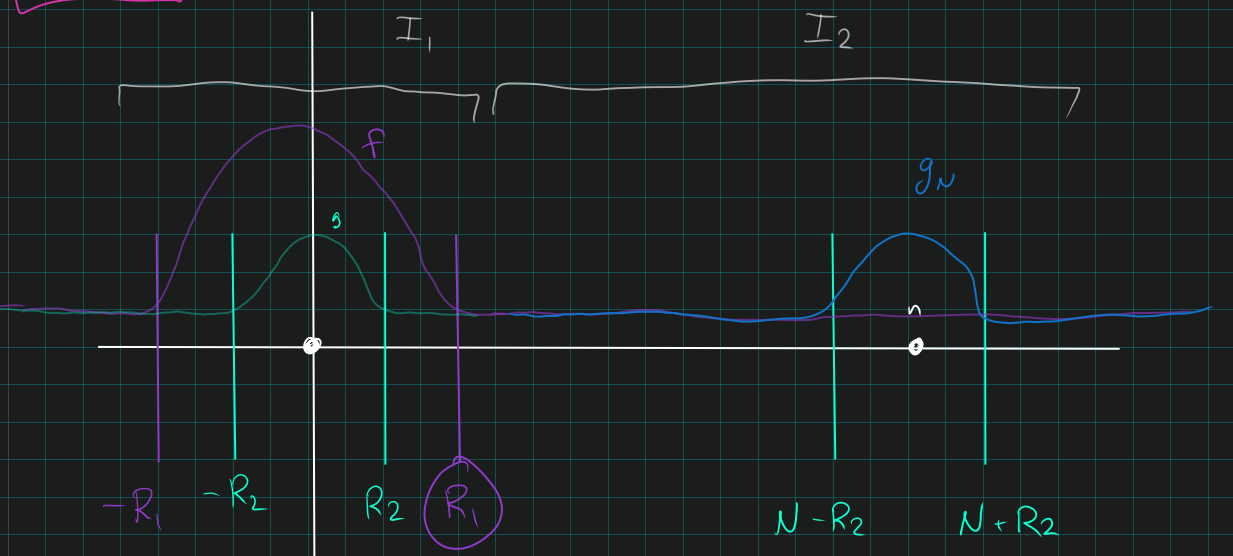
\includegraphics{figures/densities.png}
\caption{Shifting density}
\end{figure}

\begin{itemize}
\item
  Any integral \(\int_a^b f\) can be written as
  \({\left\lVert {f} \right\rVert}_1 - O(\text{err})\).
\item
  Bounding technique:
  \begin{align*}
  a-{\varepsilon}\leq b \leq a+{\varepsilon}\implies b=a
  .\end{align*}
\end{itemize}

\end{concept}

\begin{solution}

\envlist

\begin{itemize}
\item
  Fix \({\varepsilon}\).
\item
  Using small tails for \(f, g \in L^1\), choose \(R_1, R_2 \gg 0\) so
  that
  \begin{align*}
  \int_{B_{R_1}(0)^c} {\left\lvert {f} \right\rvert} &< {\varepsilon}\\
  \int_{B_{R_2}(0)^c} {\left\lvert {g} \right\rvert} &< {\varepsilon}
  .\end{align*}

  \begin{itemize}
  \item
    Note that this implies
    \begin{align*}
    \int_{-R_1}^{R_1} {\left\lvert {f} \right\rvert} &= {\left\lVert {f} \right\rVert}_1 - 2{\varepsilon}\\
    \int_{-R_2}^{R_2} {\left\lvert {g_N} \right\rvert} &= {\left\lVert {g_N} \right\rVert} - 2{\varepsilon}
    .\end{align*}
  \item
    Also note that by translation invariance of the Lebesgue integral,
    \({\left\lVert {g} \right\rVert}_1 = {\left\lVert {g_N} \right\rVert}_1\).
  \end{itemize}
\item
  Now use \(N\) to make the densities almost disjoint: choose \(N\gg 1\)
  so that \(N-R_2 > R_1\):
\end{itemize}

\begin{figure}
\centering
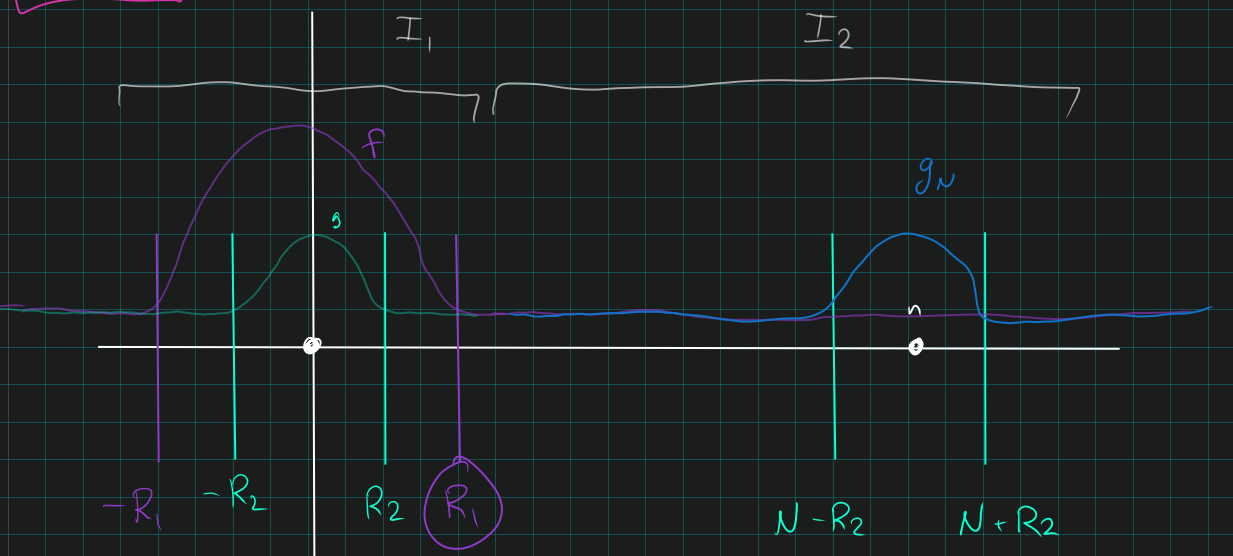
\includegraphics{figures/densities.png}
\caption{Shifting density}
\end{figure}

\begin{itemize}
\tightlist
\item
  Consider the change of variables \(x\mapsto x-N\):
  \begin{align*}
  \int_{-R_2}^{R_2} {\left\lvert {g(x)} \right\rvert}\,dx
  = \int_{N-R_2} ^{N+R_2} {\left\lvert {g(x-N)} \right\rvert} \,dx
  \coloneqq\int_{N-R_2} ^{N+R_2} {\left\lvert {g_N(x)} \right\rvert} \,dx
  .\end{align*}

  \begin{itemize}
  \tightlist
  \item
    Use this to conclude that
    \begin{align*}
    \int_{N-R_2}^{N+R_2} {\left\lvert {g_N} \right\rvert} = {\left\lVert {g_N} \right\rVert} - 2{\varepsilon}
    .\end{align*}
  \end{itemize}
\item
  Now split the integral in the problem statement at \(R_1\):
\end{itemize}

\begin{align*}
{\left\lVert {f + g_N} \right\rVert}_1 
= \int_{\mathbb{R}}{\left\lvert {f+g_N} \right\rvert} 
= \int_{-\infty}^{R_1} {\left\lvert {f+ g_N} \right\rvert}
+ \int_{R_1}^{\infty} {\left\lvert {f+ g_N} \right\rvert}
\coloneqq I_1 + I_2
.\end{align*}

\begin{itemize}
\item
  \textbf{Idea}: from the picture,

  \begin{itemize}
  \tightlist
  \item
    On \(I_1\), \(f\) is big and \(g_N\) is small
  \item
    On \(I_2\), \(f\) is small and \(g_N\) is big
  \end{itemize}
\item
  Casework: estimate \(I_1, I_2\) separately, bounding from above and
  below.
\item
  \(I_1\) upper bound:
  \begin{align*}
  I_1 
  &\coloneqq\int_{-\infty}^{R_1} {\left\lvert {f + g_N} \right\rvert} \\
  &\leq \int_{-\infty}^{R_1} {\left\lvert {f} \right\rvert} + {\left\lvert {g_N} \right\rvert} \\
  &= \int_{-\infty}^{R_1} {\left\lvert {f} \right\rvert} + \int_{-\infty}^{R_1} {\left\lvert {g_N} \right\rvert} \\
  &\leq \int_{-\infty}^{R_1} {\left\lvert {f} \right\rvert} + \int_{-\infty}^{\color{green} N - R_2} {\left\lvert {g_N} \right\rvert} && R_1 < N-R_2 \\
  &= {\left\lVert {f} \right\rVert}_1 - \int_{R_1}^{\infty} {\left\lvert {f} \right\rvert} + \int_{-\infty}^{N - R_2} {\left\lvert {g_N} \right\rvert} \\
  &\leq {\left\lVert {f} \right\rVert}_1 - \int_{R_1}^{\infty} {\left\lvert {f} \right\rvert} + {\varepsilon}\\
  &\leq {\left\lVert {f} \right\rVert}_1 + {\varepsilon}
  .\end{align*}

  \begin{itemize}
  \item
    In the last step we've used that we're subtracting off a positive
    number, so forgetting it only makes things larger.
  \item
    We've also used monotonicity of the Lebesgue integral: if
    \(A\leq B\), then \((c, A) \subseteq (c, B)\) and
    \(\int_{c}^A {\left\lvert {f} \right\rvert} \leq \int_c^B {\left\lvert {f} \right\rvert}\)
    since \({\left\lvert {f} \right\rvert}\) is positive.
  \end{itemize}
\item
  \(I_1\) lower bound:
  \begin{align*}
  I_1 
  &\coloneqq\int_{-\infty}^{R_1} {\left\lvert {f + g_N} \right\rvert} \\
  &\geq \int_{-\infty}^{R_1} {\left\lvert {f} \right\rvert} - {\left\lvert {g_N} \right\rvert} \\
  &= \int_{-\infty}^{R_1} {\left\lvert {f} \right\rvert} - \int_{-\infty}^{R_1} {\left\lvert {g_N} \right\rvert} \\
  &\geq \int_{-\infty}^{R_1} {\left\lvert {f} \right\rvert} - \int_{-\infty}^{\color{green} N-R_2} {\left\lvert {g_N} \right\rvert} && R_1 < N-R_2 \\
  &= {\left\lVert {f} \right\rVert}_1 - \int_{R_1}^{ \infty } {\left\lvert {f} \right\rvert} - \int_{- \infty }^{N-R_2} {\left\lvert {g_N} \right\rvert} \\
  &\geq {\left\lVert {f} \right\rVert}_1 - {\varepsilon}- {\varepsilon}\\
  &= {\left\lVert {f} \right\rVert}_1 - 2{\varepsilon}
  .\end{align*}

  \begin{itemize}
  \tightlist
  \item
    Now we've used that the integral with \(g_N\) comes in with a
    negative sign, so extending the range of integration only makes
    things \emph{smaller}. We've also used the \({\varepsilon}\) bound
    on both \(f\) and \(g_N\) here, and both are tail estimates.
  \end{itemize}
\item
  Taken together we conclude
  \begin{align*}
  {\left\lVert {f} \right\rVert}_1 - 2{\varepsilon}
  \leq I_1
  \leq {\left\lVert {f} \right\rVert}_1 && {\varepsilon}\to 0 \implies  I_1 = {\left\lVert {f} \right\rVert}_1
  .\end{align*}
\item
  \(I_2\) lower bound:
  \begin{align*}
  I_2 
  &\coloneqq\int_{R_1}^{\infty} {\left\lvert {f + g_N} \right\rvert} \\
  &\leq \int_{R_1}^{\infty} {\left\lvert {f} \right\rvert} + \int_{R_1}^{\infty} {g_N} \\
  &\leq \int_{R_1}^{\infty} {\left\lvert {f} \right\rvert} + {\left\lVert {g_N} \right\rVert}_1 - \int_{-\infty}^{R_1} {\left\lvert {g_N} \right\rvert} \\
  &\leq {\varepsilon}+ {\left\lVert {g_N} \right\rVert}_1 - \int_{-\infty}^{R_1} {\left\lvert {g_N} \right\rvert} \\
  &\leq {\varepsilon}+ {\left\lVert {g_N} \right\rVert}_1 \\
  &= {\varepsilon}+ {\left\lVert {g} \right\rVert}_1 
  .\end{align*}

  \begin{itemize}
  \tightlist
  \item
    Here we've again thrown away negative terms, only increasing the
    bound, and used the tail estimate on \(f\).
  \end{itemize}
\item
  \(I_2\) upper bound:
\end{itemize}

\begin{align*}
I_2 
&\coloneqq\int_{R_1}^{\infty} {\left\lvert {f + g_N} \right\rvert} \\
&= \int_{R_1}^{\infty} {\left\lvert {g_N + f} \right\rvert} \\
&\geq \int_{R_1}^{\infty} {\left\lvert {g_N} \right\rvert} - \int_{R_1}^{\infty} {\left\lvert {f} \right\rvert} \\
&=  {\left\lVert {g_N} \right\rVert} - \int_{-\infty}^{R_1} {\left\lvert {g_N} \right\rvert} - \int_{R_1}^{\infty} {\left\lvert {f} \right\rvert} \\
&\geq  {\left\lVert {g_N} \right\rVert} - 2{\varepsilon}
.\end{align*}

\begin{itemize}
\item
  Here we've swapped the order under the absolute value, and used the
  tail estimates on both \(g\) and \(f\).
\item
  Taken together:
  \begin{align*}
  {\left\lVert {g} \right\rVert}_1 - {\varepsilon}\leq I_2 \leq {\left\lVert {g} \right\rVert}_1 + 2{\varepsilon}
  .\end{align*}
\item
  Note that we have two inequalities:
  \begin{align*}
  {\left\lVert {f} \right\rVert}_1 - 2{\varepsilon}&\leq \int_{-\infty}^{R_1} {\left\lvert {f -g_N} \right\rvert} \leq {\left\lVert {f} \right\rVert}_1 + {\varepsilon}\\
  {\left\lVert {g} \right\rVert}_1 - 2{\varepsilon}&\leq \int^{\infty}_{R_1} {\left\lvert {f -g_N} \right\rvert} \leq {\left\lVert {g} \right\rVert}_1 + {\varepsilon}
  .\end{align*}
\item
  Add these to obtain
  \begin{align*}
  {\left\lVert {f} \right\rVert}_1 + {\left\lVert {g} \right\rVert}_1 - 4{\varepsilon}\leq I_1 + I_2 \coloneqq{\left\lVert {f - g_N} \right\rVert}_1 \leq {\left\lVert {f} \right\rVert} + {\left\lVert {g} \right\rVert}_1 + 2{\varepsilon}
  .\end{align*}
\item
  Check that as \(N\to \infty\) as \({\varepsilon}\to 0\) to yield the
  result.
\end{itemize}

\end{solution}

\hypertarget{fall-2020-4-work}{%
\subsection{\texorpdfstring{Fall 2020 \# 4
\(\work\)}{Fall 2020 \# 4 \textbackslash work}}\label{fall-2020-4-work}}

Prove that if \(xf(x) \in L^1({\mathbb{R}})\), then
\begin{align*}  
F(y) \coloneqq\int f(x) \cos(yx)\,  dx
\end{align*}
defines a \(C^1\) function.

\hypertarget{fubini-tonelli}{%
\section{Fubini-Tonelli}\label{fubini-tonelli}}

\hypertarget{spring-2020-4-done}{%
\subsection{\texorpdfstring{Spring 2020 \# 4
\(\done\)}{Spring 2020 \# 4 \textbackslash done}}\label{spring-2020-4-done}}

Let \(f, g\in L^1({\mathbb{R}})\). Argue that
\(H(x, y) \coloneqq f(y) g(x-y)\) defines a function in
\(L^1({\mathbb{R}}^2)\) and deduce from this fact that
\begin{align*}
(f\ast g)(x) \coloneqq\int_{\mathbb{R}}f(y) g(x-y) \,dy
\end{align*}
defines a function in \(L^1({\mathbb{R}})\) that satisfies
\begin{align*}
{\left\lVert {f\ast g} \right\rVert}_1 \leq {\left\lVert {f} \right\rVert}_1 {\left\lVert {g} \right\rVert}_1
.\end{align*}

\begin{strategy}

Just do it! Sort out the justification afterward. Use Tonelli.

\end{strategy}

\begin{concept}

\envlist

\begin{itemize}
\tightlist
\item
  Tonelli: non-negative and measurable yields measurability of slices
  and equality of iterated integrals
\item
  Fubini: \(f(x, y) \in L^1\) yields \emph{integrable} slices and
  equality of iterated integrals
\item
  F/T: apply Tonelli to \({\left\lvert {f} \right\rvert}\); if finite,
  \(f\in L^1\) and apply Fubini to \(f\)
\item
  See Folland's Real Analysis II, p.~68 for a discussion of using Fubini
  \emph{and} Tonelli.
\end{itemize}

\end{concept}

\begin{solution}

\begin{itemize}
\item
  If these norms can be computed via iterated integrals, we have
  \begin{align*}
  {\left\lVert {f\ast g} \right\rVert}_1 
  &\coloneqq\int_{\mathbb{R}}{\left\lvert {(f\ast g)(x)} \right\rvert} \,dx\\
  &\coloneqq\int_{\mathbb{R}}{\left\lvert {\int_{\mathbb{R}}H(x, y) \,dy} \right\rvert} \,dx\\
  &\coloneqq\int_{\mathbb{R}}{\left\lvert {\int_{\mathbb{R}}f(y)g(x-y) \,dy} \right\rvert} \,dx\\
  &\leq \int_{\mathbb{R}}\int_{\mathbb{R}}{\left\lvert {f(y) g(x-y)} \right\rvert} \,dx\,dy\\
  &\coloneqq\int_{\mathbb{R}}\int_{\mathbb{R}}{\left\lvert {H(x ,y)} \right\rvert}\,dx\,dy\\
  &\coloneqq\int_{{\mathbb{R}}^2} {\left\lvert {H} \right\rvert} \,d\mu_{{\mathbb{R}}^2} \\
  &\coloneqq{\left\lVert {H} \right\rVert}_{L^1({\mathbb{R}}^2)}
  .\end{align*}
  So it suffices to show \({\left\lVert {H} \right\rVert}_1 < \infty\).
\item
  A preliminary computation, the validity of which we will show
  afterward:
  \begin{align*}
  {\left\lVert {H} \right\rVert}_1
  &\coloneqq{\left\lVert {H} \right\rVert}_{L^1({\mathbb{R}}^2)} \\
  &= \int _{\mathbb{R}}\qty{ \int_{\mathbb{R}}{\left\lvert {f(y)g(x-y)} \right\rvert}  \, dy } \, dx && \text{Tonelli} \\ 
  &= \int _{\mathbb{R}}\qty{ \int_{\mathbb{R}}{\left\lvert {f(y)g(x-y)} \right\rvert}  \, dx} \, dy && \text{Tonelli} \\
  &= \int _{\mathbb{R}}\qty{ \int_{\mathbb{R}}{\left\lvert {f(y)g(t)} \right\rvert}  \, dt} \, dy && \text{setting } t=x-y, \,dt = - dx \\
  &= \int _{\mathbb{R}}\qty{ \int_{\mathbb{R}}{\left\lvert {f(y)} \right\rvert}\cdot {\left\lvert {g(t)} \right\rvert}  \, dt}\, dy \\
  &= \int _{\mathbb{R}}{\left\lvert {f(y)} \right\rvert} \cdot \qty{ \int_{\mathbb{R}}{\left\lvert {g(t)} \right\rvert}  \, dt}\, dy \\
  &\coloneqq\int _{\mathbb{R}}{\left\lvert {f(y)} \right\rvert} \cdot {\left\lVert {g} \right\rVert}_1 \,dy \\
  &= {\left\lVert {g} \right\rVert}_1 \int _{\mathbb{R}}{\left\lvert {f(y)} \right\rvert} \,dy &&\text{the norm is a constant} \\
  &\coloneqq{\left\lVert {g} \right\rVert}_1 {\left\lVert {f} \right\rVert}_1  \\
  &< \infty && \text{by assumption}
  .\end{align*}
\item
  We've used Tonelli twice: to equate the integral to the iterated
  integral, and to switch the order of integration, so it remains to
  show the hypothesis of Tonelli are fulfilled.
\end{itemize}

\begin{claim}

\(H\) is measurable on \({\mathbb{R}}^2\):

\end{claim}

\begin{proof}[?]

\envlist

\begin{itemize}
\tightlist
\item
  It suffices to show \(\tilde f(x, y) \coloneqq f(y)\) and
  \(\tilde g(x, y) \coloneqq g(x-y)\) are both measurable on
  \({\mathbb{R}}^2\).

  \begin{itemize}
  \tightlist
  \item
    Then use that products of measurable functions are measurable.
  \end{itemize}
\item
  \(f \in L^1\) by assumption, and \(L^1\) functions are measurable by
  definition.
\item
  The function \((x, y) \mapsto g(x-y)\) is measurable on
  \({\mathbb{R}}^2\):

  \begin{itemize}
  \tightlist
  \item
    \(g\) is measurable on \({\mathbb{R}}\) by assumption, so the
    cylinder function \(G(x, y) \coloneqq g(x)\) on \({\mathbb{R}}^2\)
    is measurable (result from course).
  \item
    Define a linear transformation
    \begin{align*}
    T \coloneqq
    \begin{bmatrix}
    1 & -1 
    \\
    0 & 1
    \end{bmatrix}
    \in \operatorname{GL}_2({\mathbb{R}})
    && \implies \,\,\,
    T
    \begin{bmatrix}
     x 
    \\
     y 
    \end{bmatrix}
    =
    \begin{bmatrix}
    x-y   
    \\
    y  
    \end{bmatrix}
    ,\end{align*}
    and linear functions are measurable.
  \item
    Write
    \begin{align*}
    \tilde g(x-y) \coloneqq G(x-y, y) \coloneqq(G\circ T)(x, y)
    ,\end{align*}
    and compositions of measurable functions are measurable.
  \end{itemize}
\end{itemize}

\end{proof}

\begin{itemize}
\tightlist
\item
  Apply \textbf{Tonelli} to \({\left\lvert {H} \right\rvert}\)

  \begin{itemize}
  \tightlist
  \item
    \(H\) measurable implies \({\left\lvert {H} \right\rvert}\) is
    measurable.
  \item
    \({\left\lvert {H} \right\rvert}\) is non-negative.
  \item
    So the iterated integrals are equal in the extended sense
  \item
    The calculation shows the iterated integral is finite, so
    \(\int {\left\lvert {H} \right\rvert}\) is finite and \(H\) is thus
    integrable on \({\mathbb{R}}^2\).
  \end{itemize}
\end{itemize}

\begin{quote}
Note: Fubini is not needed, since we're not calculating the actual
integral, just showing \(H\) is integrable.
\end{quote}

\end{solution}

\hypertarget{spring-2019-4-done}{%
\subsection{\texorpdfstring{Spring 2019 \# 4
\(\done\)}{Spring 2019 \# 4 \textbackslash done}}\label{spring-2019-4-done}}

Let \(f\) be a non-negative function on \({\mathbb{R}}^n\) and
\(\mathcal A = \{(x, t) ∈ {\mathbb{R}}^n \times {\mathbb{R}}: 0 ≤ t ≤ f (x)\}\).

Prove the validity of the following two statements:

\begin{enumerate}
\def\labelenumi{\alph{enumi}.}
\item
  \(f\) is a Lebesgue measurable function on
  \({\mathbb{R}}^n \iff \mathcal A\) is a Lebesgue measurable subset of
  \({\mathbb{R}}^{n+1}\)
\item
  If \(f\) is a Lebesgue measurable function on \({\mathbb{R}}^n\), then
  \begin{align*}
  m(\mathcal{A})=\int _{{\mathbb{R}}^{n}} f(x) d x=\int_{0}^{\infty} m\left(\left\{x \in {\mathbb{R}}^{n}: f(x) \geq t\right\}\right) dt
  \end{align*}
\end{enumerate}

\begin{concept}

\envlist

\begin{itemize}
\tightlist
\item
  See Stein and Shakarchi p.82 corollary 3.3.
\item
  Tonelli
\item
  Important trick!
  \(\left\{{(x, t) {~\mathrel{\Big|}~}0\leq t \leq f(x)}\right\} = \left\{{ f(x) \geq t}\right\} \cap\left\{{ t\geq 0 }\right\}\)
\end{itemize}

\end{concept}

\begin{solution}

\envlist

\begin{proof}[a, $\implies$]

\(\implies\):

\begin{itemize}
\tightlist
\item
  Suppose \(f:{\mathbb{R}}^n\to {\mathbb{R}}\) is a measurable function.
\item
  Rewrite \(A\):
  \begin{align*}
  A 
  &= \left\{{ (x, t) \in {\mathbb{R}}^d \times{\mathbb{R}}{~\mathrel{\Big|}~}0\leq t \leq f(x) }\right\} \\
  &= \left\{{ (x, t) \in {\mathbb{R}}^d \times{\mathbb{R}}{~\mathrel{\Big|}~}0 \leq t < \infty }\right\} 
  \cap\left\{{ (x, t) \in {\mathbb{R}}^d\times{\mathbb{R}}{~\mathrel{\Big|}~}t\leq f(x) }\right\} \\
  &= \qty{ {\mathbb{R}}^d \times[0, \infty) } 
  \cap\left\{{ (x, t) \in {\mathbb{R}}^d\times{\mathbb{R}}{~\mathrel{\Big|}~}f(x) -t \geq 0  }\right\} \\
  &\coloneqq\qty{ {\mathbb{R}}^d \times[0, \infty) } \cap H^{-1}\qty{[0, \infty)}
  ,\end{align*}
  where we define
  \begin{align*}
  H: {\mathbb{R}}^d \times{\mathbb{R}}&\to {\mathbb{R}}\\
  (x, t) &\mapsto f(x) - t
  .\end{align*}

  \begin{itemize}
  \tightlist
  \item
    Note: this is ``clearly'' measurable!
  \end{itemize}
\item
  If we can show both sets are measurable, we're done, since
  \(\sigma{\hbox{-}}\)algebras are closed under countable intersections.
\item
  The first set is measurable since it is a Borel set in
  \({\mathbb{R}}^{d+1}\).
\item
  For the same reason, it suffices to show \(H\) is a measurable
  function.
\item
  Define cylinder functions
  \begin{align*}
  F: {\mathbb{R}}^d \times{\mathbb{R}}&\to {\mathbb{R}}\\
  (x, t) &\mapsto f(x)
  \end{align*}
  and
  \begin{align*}
  G: {\mathbb{R}}^d \times{\mathbb{R}}&\to {\mathbb{R}}\\
  (x, t) &\mapsto t
  \end{align*}

  \begin{itemize}
  \tightlist
  \item
    \(F\) is a cylinder of \(f\), and since \(f\) is measurable by
    assumption, \(F\) is measurable.
  \item
    \(G\) is a cylinder on the identity for \({\mathbb{R}}\), which is
    measurable, so \(G\) is measurable.
  \end{itemize}
\item
  Define
  \begin{align*}
  H: {\mathbb{R}}^d &\to {\mathbb{R}}\\
  (x, t) &\mapsto F(x, t) - G(x, t) \coloneqq f(x) - t
  ,\end{align*}
  which are linear combinations of measurable functions and thus
  measurable.
\end{itemize}

\end{proof}

\begin{proof}[a, $\impliedby$]

\(\impliedby\):

\begin{itemize}
\item
  Suppose \({\mathcal{A}}\) is a measurable set.
\item
  A corollary of Tonelli applied to \(\chi_X\): if \(E\) is measurable,
  then for a.e. \(t\) the following slice is measurable:
  \begin{align*}
  {\mathcal{A}}_t \coloneqq\left\{{ x \in {\mathbb{R}}^d {~\mathrel{\Big|}~}(x,t) \in {\mathcal{A}}}\right\}
  &= \left\{{x\in {\mathbb{R}}^d {~\mathrel{\Big|}~}f(x) \geq t \geq 0}\right\} \\
  &= f^{-1}\qty{[t, \infty)}
  .\end{align*}

  \begin{itemize}
  \tightlist
  \item
    But maybe this isn't enough, because we need
    \(f^{-1}\qty{[\alpha, \infty)}\) for \emph{all} \(\alpha\)
  \end{itemize}
\item
  But the other slice is also measurable for a.e. \(x\):
  \begin{align*}
  {\mathcal{A}}_x 
  &\coloneqq\left\{{ t\in {\mathbb{R}}{~\mathrel{\Big|}~}(x, t) \in {\mathcal{A}}}\right\} \\
  &= \left\{{ t\in {\mathbb{R}}{~\mathrel{\Big|}~}0 \leq t \leq f(x) }\right\} \\
  &= \left\{{ t\in {\mathbb{R}}{~\mathrel{\Big|}~}t\in [0, f(x)]  }\right\} \\
  &= [0, f(x)]
  .\end{align*}
\item
  Moreover the function \(x\mapsto m({\mathcal{A}}_x)\) is a measurable
  function of \(x\)
\item
  Now note \(m({\mathcal{A}}_x) = f(x) - 0 = f(x)\), so \(f\) must be
  measurable.
\end{itemize}

\end{proof}

\begin{proof}[of b]

\envlist

\begin{itemize}
\item
  Writing down what the slices are
  \begin{align*}
  \mathcal{A} &= \left\{{(x, t) \in {\mathbb{R}}^n\times{\mathbb{R}}{~\mathrel{\Big|}~}0 \leq t \leq f(x)}\right\} 
  \\
  \mathcal{A}_t &= \left\{{x
  \in {\mathbb{R}}^n {~\mathrel{\Big|}~}t\leq f(x) }\right\}
  .\end{align*}
\item
  Then
  \begin{align*}
  \int_{{\mathbb{R}}^n} f(x) ~dx 
  &= \int_{{\mathbb{R}}^n} \int_0^{f(x)} 1 ~dt~dx \\
  &= \int_{{\mathbb{R}}^n} \int_{0}^\infty \chi_\mathcal{A} ~dt~dx \\
  &\overset{F.T.}= \int_{0}^\infty \int_{{\mathbb{R}}^n} \chi_\mathcal{A} ~dx~dt\\
  &= \int_0^\infty m(\mathcal{A}_t) ~dt
  ,\end{align*}
  where we just use that \(\int \int \chi_\mathcal{A} = m(\mathcal{A})\)
\item
  By Tonelli, all of these integrals are equal.

  \begin{itemize}
  \tightlist
  \item
    This is justified because \(f\) was assumed measurable on
    \({\mathbb{R}}^n\), thus by (a) \(\mathcal{A}\) is a measurable set
    and thus \(\chi_A\) is a measurable function on
    \({\mathbb{R}}^n\times{\mathbb{R}}\).
  \end{itemize}
\end{itemize}

\end{proof}

\end{solution}

\hypertarget{fall-2018-5-done}{%
\subsection{\texorpdfstring{Fall 2018 \# 5
\(\done\)}{Fall 2018 \# 5 \textbackslash done}}\label{fall-2018-5-done}}

Let \(f \geq 0\) be a measurable function on \({\mathbb{R}}\). Show that
\begin{align*}
\int _{{\mathbb{R}}} f = \int _{0}^{\infty} m(\{x: f(x)>t\}) dt
\end{align*}

\begin{concept}

\envlist

\begin{itemize}
\tightlist
\item
  Claim: If \(E\subseteq {\mathbb{R}}^a \times{\mathbb{R}}^b\) is a
  measurable set, then for almost every \(y\in {\mathbb{R}}^b\), the
  slice \(E^y\) is measurable and
  \begin{align*}
  m(E) = \int_{{\mathbb{R}}^b} m(E^y) \,dy
  .\end{align*}

  \begin{itemize}
  \tightlist
  \item
    Set \(g = \chi_E\), which is non-negative and measurable, so apply
    Tonelli.
  \item
    Conclude that \(g^y = \chi_{E^y}\) is measurable, the function
    \(y\mapsto \int g^y(x)\, dx\) is measurable, and
    \(\int \int g^y(x)\,dx \,dy = \int g\).
  \item
    But \(\int g = m(E)\) and
    \(\int\int g^y(x) \,dx\,dy = \int m(E^y)\,dy\).
  \end{itemize}
\end{itemize}

\end{concept}

\begin{solution}

\envlist

\begin{quote}
Note: \(f\) is a function \({\mathbb{R}}\to {\mathbb{R}}\) in the
original problem, but here I've assumed
\(f:{\mathbb{R}}^n\to {\mathbb{R}}\).
\end{quote}

\begin{itemize}
\item
  Since \(f\geq 0\), set
  \begin{align*}
  E\coloneqq\left\{{(x, t) \in {\mathbb{R}}^{n} \times{\mathbb{R}}{~\mathrel{\Big|}~}f(x) > t}\right\}
  = \left\{{(x, t) \in {\mathbb{R}}^n \times{\mathbb{R}}{~\mathrel{\Big|}~}0 \leq t < f(x)}\right\}
  .\end{align*}
\item
  Claim: since \(f\) is measurable, \(E\) is measurable and thus
  \(m(E)\) makes sense.

  \begin{itemize}
  \tightlist
  \item
    Since \(f\) is measurable, \(F(x, t) \coloneqq t - f(x)\) is
    measurable on \({\mathbb{R}}^n \times{\mathbb{R}}\).
  \item
    Then write
    \(E = \left\{{F < 0}\right\} \cap\left\{{t\geq 0}\right\}\) as an
    intersection of measurable sets.
  \end{itemize}
\item
  We have slices
  \begin{align*}
  E^t &\coloneqq\left\{{x\in {\mathbb{R}}^n {~\mathrel{\Big|}~}(x, t) \in E}\right\} = \left\{{x\in {\mathbb{R}}^n {~\mathrel{\Big|}~}0 \leq t < f(x)}\right\} \\
  E^x &\coloneqq\left\{{t\in {\mathbb{R}}{~\mathrel{\Big|}~}(x, t) \in E}\right\} = \left\{{t\in {\mathbb{R}}{~\mathrel{\Big|}~}0 \leq t \leq f(x)}\right\} = [0, f(x)]
  .\end{align*}

  \begin{itemize}
  \tightlist
  \item
    \(E_t\) is precisely the set that appears in the original RHS
    integrand.
  \item
    \(m(E^x) = f(x)\).
  \end{itemize}
\item
  Claim: \(\chi_E\) satisfies the conditions of Tonelli, and thus
  \(m(E) = \int \chi_E\) is equal to any iterated integral.

  \begin{itemize}
  \tightlist
  \item
    Non-negative: clear since \(0\leq \chi_E \leq 1\)
  \item
    Measurable: characteristic functions of measurable sets are
    measurable.
  \end{itemize}
\item
  Conclude:

  \begin{enumerate}
  \def\labelenumi{\arabic{enumi}.}
  \tightlist
  \item
    For almost every \(x\), \(E^x\) is a measurable set,
    \(x\mapsto m(E^x)\) is a measurable function, and
    \(m(E) = \int_{{\mathbb{R}}^n} m(E^x) \, dx\)
  \item
    For almost every \(t\), \(E^t\) is a measurable set,
    \(t\mapsto m(E^t)\) is a measurable function, and
    \(m(E) = \int_{{\mathbb{R}}} m(E^t) \, dt\)
  \end{enumerate}
\item
  On one hand,
  \begin{align*}
  m(E) 
  &= \int_{{\mathbb{R}}^{n+1}} \chi_E(x, t) \\
  &= \int_{{\mathbb{R}}} \int_{{\mathbb{R}}^n} \chi_E(x, t) \,dt \,dx \quad\text{by Tonelli}\\
  &= \int_{{\mathbb{R}}^n} m(E^x) \,dx \quad\text{first conclusion}\\
  &= \int_{{\mathbb{R}}^n} f(x) \,dx 
  .\end{align*}
\item
  On the other hand,
  \begin{align*}
  m(E) 
  &= \int_{{\mathbb{R}}^{n+1}} \chi_E(x, t) \\
  &= \int_{\mathbb{R}}\int_{{\mathbb{R}}^n} \chi_E(x, t) \, dx \,dt \quad\text{by Tonelli} \\
  &= \int_{\mathbb{R}}m(E^t) \,dt \quad\text{second conclusion}
  .\end{align*}
\item
  Thus
  \begin{align*}
  \int_{{\mathbb{R}}^n} f \,dx = m(E) = \int_{\mathbb{R}}m(E^t) \,dt = \int_{\mathbb{R}}m\qty{\left\{{x{~\mathrel{\Big|}~}f(x) > t}\right\}}
  .\end{align*}
\end{itemize}

\end{solution}

\hypertarget{fall-2015-5-work}{%
\subsection{\texorpdfstring{Fall 2015 \# 5
\(\work\)}{Fall 2015 \# 5 \textbackslash work}}\label{fall-2015-5-work}}

Let \(f, g \in L^1({\mathbb{R}})\) be Borel measurable.

\begin{enumerate}
\def\labelenumi{\arabic{enumi}.}
\tightlist
\item
  Show that
\end{enumerate}

\begin{itemize}
\tightlist
\item
  The function
  \begin{align*}F(x, y) \coloneqq f(x-y) g(y)\end{align*}
  is Borel measurable on \({\mathbb{R}}^2\), and
\item
  For almost every \(y\in {\mathbb{R}}\),
  \begin{align*}F_y(x) \coloneqq f(x-y)g(y)\end{align*}
  is integrable with respect to \(y\).
\end{itemize}

\begin{enumerate}
\def\labelenumi{\arabic{enumi}.}
\setcounter{enumi}{1}
\tightlist
\item
  Show that \(f\ast g \in L^1({\mathbb{R}})\) and
  \begin{align*}
  \|f * g\|_{1} \leq \|f\|_{1} \|g\|_{1}
  \end{align*}
\end{enumerate}

\hypertarget{spring-2014-5-work}{%
\subsection{\texorpdfstring{Spring 2014 \# 5
\(\work\)}{Spring 2014 \# 5 \textbackslash work}}\label{spring-2014-5-work}}

Let \(f, g \in L^1([0, 1])\) and for all \(x\in [0, 1]\) define
\begin{align*}
F(x) \coloneqq\int _{0}^{x} f(y) \, dy 
{\quad \operatorname{and} \quad}
G(x)\coloneqq\int _{0}^{x} g(y) \, dy.
\end{align*}

Prove that
\begin{align*}
\int _{0}^{1} F(x) g(x) \, dx = 
F(1) G(1) - \int _{0}^{1} f(x) G(x) \, dx
\end{align*}

\hypertarget{spring-2021-6}{%
\subsection{Spring 2021 \# 6}\label{spring-2021-6}}

\begin{warnings}

This problem may be much harder than expected. Recommended skip.

\end{warnings}

Let \(f: {\mathbb{R}}\times{\mathbb{R}}\to {\mathbb{R}}\) be a
measurable function and for \(x\in {\mathbb{R}}\) define the set
\begin{align*}
E_x \coloneqq\left\{{ y\in {\mathbb{R}}{~\mathrel{\Big|}~}\mu\qty{ z\in {\mathbb{R}}{~\mathrel{\Big|}~}f(x,z) = f(x, y) } > 0 }\right\} 
.\end{align*}
Show that the following set is a measurable subset of
\({\mathbb{R}}\times{\mathbb{R}}\):
\begin{align*}
E \coloneqq\displaystyle\bigcup_{x\in {\mathbb{R}}} \left\{{ x }\right\} \times E_x
.\end{align*}

\begin{quote}
Hint: consider the measurable function
\(h(x,y,z) \coloneqq f(x, y) - f(x, z)\).
\end{quote}

\hypertarget{l2-and-fourier-analysis}{%
\section{\texorpdfstring{\(L^2\) and Fourier
Analysis}{L\^{}2 and Fourier Analysis}}\label{l2-and-fourier-analysis}}

\hypertarget{spring-2020-6-done}{%
\subsection{\texorpdfstring{Spring 2020 \# 6
\(\done\)}{Spring 2020 \# 6 \textbackslash done}}\label{spring-2020-6-done}}

\hypertarget{a-1}{%
\subsubsection{a}\label{a-1}}

Show that
\begin{align*}
L^2([0, 1]) \subseteq L^1([0, 1]) {\quad \operatorname{and} \quad} \ell^1({\mathbb{Z}}) \subseteq \ell^2({\mathbb{Z}})
.\end{align*}

\hypertarget{b-1}{%
\subsubsection{b}\label{b-1}}

For \(f\in L^1([0, 1])\) define
\begin{align*}
\widehat{f}(n) \coloneqq\int _0^1 f(x) e^{-2\pi i n x} \, dx
.\end{align*}

Prove that if \(f\in L^1([0, 1])\) and
\(\left\{{\widehat{f}(n)}\right\} \in \ell^1({\mathbb{Z}})\) then
\begin{align*}
S_N f(x) \coloneqq\sum_{{\left\lvert {n} \right\rvert} \leq N} \widehat{f} (n) e^{2 \pi i n x}
.\end{align*}
converges uniformly on \([0, 1]\) to a continuous function \(g\) such
that \(g = f\) almost everywhere.

\begin{quote}
Hint: One approach is to argue that if \(f\in L^1([0, 1])\) with
\(\left\{{\widehat{f} (n)}\right\} \in \ell^1({\mathbb{Z}})\) then
\(f\in L^2([0, 1])\).
\end{quote}

\begin{solution}

\hfill

\begin{concept}

\hfill

\begin{itemize}
\tightlist
\item
  For \(e_n(x) \coloneqq e^{2\pi i n x}\), the set
  \(\left\{{e_n}\right\}\) is an orthonormal basis for \(L^2([0, 1])\).
\item
  For any orthonormal sequence in a Hilbert space, we have Bessel's
  inequality:
  \begin{align*}
  \sum_{k=1}^{\infty}\left|\left\langle x, e_{k}\right\rangle\right|^{2} \leq\|x\|^{2}
  .\end{align*}
\item
  When \(\left\{{e_n}\right\}\) is a basis, the above is an
  \emph{equality} (Parseval)
\item
  Arguing uniform convergence: since
  \(\left\{{\widehat{f}(n)}\right\} \in \ell^1({\mathbb{Z}})\), we
  should be able to apply the \(M\) test.
\end{itemize}

\end{concept}

\hypertarget{a-2}{%
\subsubsection{a}\label{a-2}}

Claim: \(\ell^1({\mathbb{Z}}) \subseteq \ell^2({\mathbb{Z}})\).

\begin{itemize}
\tightlist
\item
  Set
  \(\mathbf{c} = \left\{{c_k {~\mathrel{\Big|}~}k\in {\mathbb{Z}}}\right\} \in \ell^1({\mathbb{Z}})\).
\item
  It suffices to show that if
  \(\sum_{k\in {\mathbb{Z}}} {\left\lvert {c_k} \right\rvert} < \infty\)
  then
  \(\sum_{k\in {\mathbb{Z}}} {\left\lvert {c_k} \right\rvert}^2 < \infty\).
\item
  Let
  \(S = \left\{{c_k {~\mathrel{\Big|}~}{\left\lvert {c_k} \right\rvert} \leq 1}\right\}\),
  then
  \(c_k \in S \implies {\left\lvert {c_k} \right\rvert}^2 \leq {\left\lvert {c_k} \right\rvert}\)
\item
  Claim: \(S^c\) can only contain finitely many elements, all of which
  are finite.

  \begin{itemize}
  \tightlist
  \item
    If not, either \(S^c \coloneqq\left\{{c_j}\right\}_{j=1}^\infty\) is
    infinite with every \({\left\lvert {c_j} \right\rvert} > 1\), which
    forces
    \begin{align*}\sum_{c_k\in S^c} {\left\lvert {c_k} \right\rvert} = \sum_{j=1}^\infty {\left\lvert {c_j} \right\rvert} > \sum_{j=1}^\infty 1 = \infty.\end{align*}
  \item
    If any \(c_j = \infty\), then
    \(\sum_{k\in {\mathbb{Z}}} {\left\lvert {c_k} \right\rvert} \geq c_j = \infty\).
  \end{itemize}
\item
  So \(S^c\) is a finite set of finite integers, let
  \(N = \max \left\{{{\left\lvert {c_j} \right\rvert}^2 {~\mathrel{\Big|}~}c_j \in S^c}\right\} < \infty\).
\item
  Rewrite the sum
  \begin{align*}
  \sum_{k\in {\mathbb{Z}}} {\left\lvert {c_k} \right\rvert}^2 
  &= \sum_{c_k\in S} {\left\lvert {c_k} \right\rvert}^2 + \sum_{c_k \in S^c} {\left\lvert {c_k} \right\rvert}^2 \\
  &\leq \sum_{c_k\in S} {\left\lvert {c_k} \right\rvert} + \sum_{c_k \in S^c} {\left\lvert {c_k} \right\rvert}^2 \\
  &\leq \sum_{k\in {\mathbb{Z}}} {\left\lvert {c_k} \right\rvert} + \sum_{c_k \in S^c} {\left\lvert {c_k} \right\rvert}^2 \quad\text{since the ${\left\lvert {c_k} \right\rvert}$ are all positive} \\
  &= {\left\lVert {\mathbf{c}} \right\rVert}_{\ell^1} + \sum_{c_k \in S^c} {\left\lvert {c_k} \right\rvert}^2 \\
  &\leq {\left\lVert {\mathbf{c}} \right\rVert}_{\ell^1} + {\left\lvert {S^c} \right\rvert}\cdot N \\
  &< \infty
  .\end{align*}
\end{itemize}

Claim: \(L^2([0, 1]) \subseteq L^1([0, 1])\).

\begin{itemize}
\item
  It suffices to show that
  \(\int {\left\lvert {f} \right\rvert}^2 < \infty \implies \int {\left\lvert {f} \right\rvert} < \infty\).
\item
  Define
  \(S = \left\{{x\in [0, 1] {~\mathrel{\Big|}~}{\left\lvert {f(x)} \right\rvert} \leq 1}\right\}\),
  then
  \(x\in S^c \implies {\left\lvert {f(x)} \right\rvert}^2 \geq {\left\lvert {f(x)} \right\rvert}\).
\item
  Break up the integral:
  \begin{align*}
  \int_{\mathbb{R}}{\left\lvert {f} \right\rvert} 
  &= \int_S {\left\lvert {f} \right\rvert} + \int_{S^c} {\left\lvert {f} \right\rvert} \\
  &\leq \int_S {\left\lvert {f} \right\rvert} + \int_{S^c} {\left\lvert {f} \right\rvert}^2 \\
  &\leq \int_S {\left\lvert {f} \right\rvert} + {\left\lVert {f} \right\rVert}_2 \\
  &\leq \sup_{x\in S}\left\{{{\left\lvert {f(x)} \right\rvert}}\right\} \cdot \mu(S) + {\left\lVert {f} \right\rVert}_2 \\
  &= 1 \cdot \mu(S) + {\left\lVert {f} \right\rVert}_2 \quad\text{by definition of } S\\
  &\leq 1 \cdot \mu([0, 1]) + {\left\lVert {f} \right\rVert}_2 \quad\text{since } S\subseteq [0, 1] \\
  &= 1 + {\left\lVert {f} \right\rVert}_2 \\
  &< \infty
  .\end{align*}
\end{itemize}

\begin{quote}
Note: this proof shows \(L^2(X) \subseteq L^1(X)\) whenever
\(\mu(X) < \infty\).
\end{quote}

\end{solution}

\hypertarget{fall-2017-5-done}{%
\subsection{\texorpdfstring{Fall 2017 \# 5
\(\done\)}{Fall 2017 \# 5 \textbackslash done}}\label{fall-2017-5-done}}

Let \(\phi\) be a compactly supported smooth function that vanishes
outside of an interval \([-N, N]\) such that
\(\int _{{\mathbb{R}}} \phi(x) \, dx = 1\).

For \(f\in L^1({\mathbb{R}})\), define
\begin{align*}
K_{j}(x) \coloneqq j \phi(j x), 
\qquad 
f \ast K_{j}(x) \coloneqq\int_{{\mathbb{R}}} f(x-y) K_{j}(y) \, dy
\end{align*}
and prove the following:

\begin{enumerate}
\def\labelenumi{\arabic{enumi}.}
\item
  Each \(f\ast K_j\) is smooth and compactly supported.
\item

  \begin{align*}
  \lim _{j \to \infty} {\left\lVert {f * K_{j}-f} \right\rVert}_{1} = 0
  \end{align*}
\end{enumerate}

\begin{quote}
Hint:
\begin{align*}
\lim _{y \to 0} \int _{{\mathbb{R}}} |f(x-y)-f(x)| dy = 0
\end{align*}
\end{quote}

\todo[inline]{Add concepts.}

\begin{solution}

\hfill

\begin{concept}

\hfill

\begin{itemize}
\tightlist
\item
  ?
\end{itemize}

\end{concept}

\hypertarget{a-3}{%
\subsubsection{a}\label{a-3}}

\textbf{Lemma:} If \(\phi \in C_c^1\), then
\((f \ast \phi)' = f \ast \phi'\) almost everywhere.

\emph{Silly Proof:}

\begin{align*}
\mathcal{F}(
    (f \ast \phi)'
 )
&= 2\pi i \xi ~\mathcal{F}(f\ast \phi) \\
&= 2\pi i \xi ~ \mathcal{F}(f) ~ \mathcal{F}(\phi) \\
&= \mathcal{F}(f) \cdot \left( 2\pi i \xi ~\mathcal{F}(\phi)\right) \\
&= \mathcal{F}(f) \cdot \mathcal{F}(\phi') \\
&= \mathcal{F}(f\ast \phi')
.\end{align*}

\emph{Actual proof}:

\begin{align*}
(f\ast \phi)'(x)
&= (\phi\ast f)'(x) \\
&= \lim_{h\to 0} \frac{(\phi\ast f)'(x+h) - (\phi\ast f)'(x)}{h} \\
&= \lim_{h\to 0} \int \frac{\phi(x + h - y) - \phi(x - y)}{h} f(y) \\
&\overset{DCT}=  \int \lim_{h\to 0} \frac{\phi(x + h - y) - \phi(x - y)}{h} f(y) \\
&= \int \phi'(x-y) f(y) \\
&= (\phi' \ast f)(x) \\
&= (f \ast \phi')(x)
.\end{align*}

To see that the DCT is justified, we can apply the MVT on the interval
\([0, h]\) to \(f\) to obtain

\begin{align*}
\frac{\phi(x + h - y) - \phi(x - y)}{h}
&= \phi'(c) \quad c\in [0, h]
,\end{align*}

and since \(\phi'\) is continuous and compactly supported, \(\phi'\) is
bounded by some \(M < \infty\) by the extreme value theorem and thus
\begin{align*}
\int {\left\lvert {\frac{\phi(x + h - y) - \phi(x - y)}{h} f(y)} \right\rvert} 
&= \int {\left\lvert {\phi'(c) f(y)} \right\rvert} \\
&\leq \int {\left\lvert {M} \right\rvert}{\left\lvert {f} \right\rvert} \\
&= {\left\lvert {M} \right\rvert} \int {\left\lvert {f} \right\rvert} < \infty
,\end{align*}

since \(f\in L^1\) by assumption, so we can take
\(g\coloneqq{\left\lvert {M} \right\rvert} {\left\lvert {f} \right\rvert}\)
as the dominating function.

Applying this theorem infinitely many times shows that \(f\ast \phi\) is
smooth.

To see that \(f\ast \phi\) is compactly supported, approximate \(f\) by
a \emph{continuous} compactly supported function \(h\), so
\({\left\lVert {h - f} \right\rVert}_1 \overset{L^1}\to 0\).

Now let \(g_x(y) = \phi(x-y)\), and note that
\(\mathrm{supp}(g) = x - \mathrm{supp}(\phi)\) which is still compact.

But since \(\mathrm{supp}(h)\) is bounded, there is some \(N\) such that
\begin{align*}
{\left\lvert {x} \right\rvert} > N \implies A_x\coloneqq\mathrm{supp}(h) \cap\mathrm{supp}(g_x) = \emptyset
\end{align*}

and thus
\begin{align*}
(h\ast \phi)(x) 
&= \int_{\mathbb{R}}\phi(x-y) h(y)~dy \\
&= \int_{A_x} g_x(y) h(y) \\
&= 0
,\end{align*}

so \(\left\{{x {~\mathrel{\Big|}~}f\ast g(x) = 0}\right\}\) is open, and
its complement is closed and bounded and thus compact.

\hypertarget{b-2}{%
\subsubsection{b}\label{b-2}}

\begin{align*}
{\left\lVert {f\ast K_j - f} \right\rVert}_1 
&= \int {\left\lvert {\int f(x-y) K_j(y) ~dy  - f(x)} \right\rvert}~dx \\
&= \int {\left\lvert {\int f(x-y) K_j(y) ~dy  - \int f(x) K_j(y) ~ dy} \right\rvert}~dx \\
&= \int {\left\lvert {\int ( f(x-y) - f(x) ) K_j(y) ~dy } \right\rvert} ~dx \\
&\leq \int \int {\left\lvert {(f(x-y) - f(x))} \right\rvert} \cdot {\left\lvert {K_j(y)} \right\rvert} ~ dy~dx \\
&\overset{FT}= \int \int {\left\lvert {(f(x-y) - f(x))} \right\rvert} \cdot {\left\lvert {K_j(y)} \right\rvert} \mathbf{~ dx~dy}\\
&= \int {\left\lvert {K_j(y)} \right\rvert} \left( \int {\left\lvert {(f(x-y) - f(x))} \right\rvert}  ~ dx\right) ~dy \\
&= \int {\left\lvert {K_j(y)} \right\rvert} \cdot {\left\lVert {f - \tau_y f} \right\rVert}_1 ~dy
.\end{align*}

We now split the integral up into pieces.

\begin{enumerate}
\def\labelenumi{\arabic{enumi}.}
\item
  Chose \(\delta\) small enough such that
  \({\left\lvert {y} \right\rvert} < \delta \implies {\left\lVert {f - \tau_y f} \right\rVert}_1 < \varepsilon\)
  by continuity of translation in \(L^1\), and
\item
  Since \(\phi\) is compactly supported, choose \(J\) large enough such
  that
  \begin{align*}
  j > J \implies \int_{{\left\lvert {y} \right\rvert} \geq \delta} {\left\lvert {K_j(y)} \right\rvert} ~dy 
  = \int_{{\left\lvert {y} \right\rvert} \geq \delta} {\left\lvert {j\phi(jy)} \right\rvert} = 0
  \end{align*}
\end{enumerate}

Then
\begin{align*}
{\left\lVert {f\ast K_j - f} \right\rVert}_1 
&\leq 
\int {\left\lvert {K_j(y)} \right\rvert} \cdot {\left\lVert {f - \tau_y f} \right\rVert}_1 ~dy \\
&= \int_{{\left\lvert {y} \right\rvert} < \delta} {\left\lvert {K_j(y)} \right\rvert} \cdot {\left\lVert {f - \tau_y f} \right\rVert}_1 ~dy 
+ \int_{{\left\lvert {y} \right\rvert} \geq  \delta} {\left\lvert {K_j(y)} \right\rvert} \cdot {\left\lVert {f - \tau_y f} \right\rVert}_1 ~dy \\
&= \varepsilon \int_{{\left\lvert {y} \right\rvert} \geq  \delta} {\left\lvert {K_j(y)} \right\rvert} + 0 \\
&\leq \varepsilon(1) \to 0
.\end{align*}

\end{solution}

\hypertarget{spring-2017-5-work}{%
\subsection{\texorpdfstring{Spring 2017 \# 5
\(\work\)}{Spring 2017 \# 5 \textbackslash work}}\label{spring-2017-5-work}}

Let \(f, g \in L^2({\mathbb{R}})\). Prove that the formula
\begin{align*}
h(x) \coloneqq\int _{-\infty}^{\infty} f(t) g(x-t) \, dt
\end{align*}
defines a uniformly continuous function \(h\) on \({\mathbb{R}}\).

\hypertarget{spring-2015-6-work}{%
\subsection{\texorpdfstring{Spring 2015 \# 6
\(\work\)}{Spring 2015 \# 6 \textbackslash work}}\label{spring-2015-6-work}}

Let \(f \in L^1({\mathbb{R}})\) and \(g\) be a bounded measurable
function on \({\mathbb{R}}\).

\begin{enumerate}
\def\labelenumi{\arabic{enumi}.}
\tightlist
\item
  Show that the convolution \(f\ast g\) is well-defined, bounded, and
  uniformly continuous on \({\mathbb{R}}\).
\item
  Prove that one further assumes that \(g \in C^1({\mathbb{R}})\) with
  bounded derivative, then \(f\ast g \in C^1({\mathbb{R}})\) and
  \begin{align*}
  \frac{d}{d x}(f * g)=f *\left(\frac{d}{d x} g\right)
  \end{align*}
\end{enumerate}

\hypertarget{fall-2014-5-work}{%
\subsection{\texorpdfstring{Fall 2014 \# 5
\(\work\)}{Fall 2014 \# 5 \textbackslash work}}\label{fall-2014-5-work}}

\begin{enumerate}
\def\labelenumi{\arabic{enumi}.}
\item
  Let \(f \in C_c^0({\mathbb{R}}^n)\), and show
  \begin{align*}
  \lim _{t \to 0} \int_{{\mathbb{R}}^n} |f(x+t) - f(x)| \, dx = 0
  .\end{align*}
\item
  Extend the above result to \(f\in L^1({\mathbb{R}}^n)\) and show that
  \begin{align*}
  f\in L^1({\mathbb{R}}^n), \quad g\in L^\infty({\mathbb{R}}^n) \quad
  \implies f \ast g \text{ is bounded and uniformly continuous. }
  \end{align*}
\end{enumerate}

\hypertarget{fall-2020-5}{%
\subsection{Fall 2020 \# 5}\label{fall-2020-5}}

Suppose \(\phi\in L^1({\mathbb{R}})\) with
\begin{align*}  
\int \phi(x) \, dx = \alpha
.\end{align*}
For each \(\delta > 0\) and \(f\in L^1({\mathbb{R}})\), define
\begin{align*}  
A_\delta f(x) \coloneqq\int f(x-y) \delta^{-1} \phi\qty{\delta^{-1} y}\, dy
.\end{align*}

\begin{enumerate}
\def\labelenumi{\alph{enumi}.}
\item
  Prove that for all \(\delta > 0\),
  \begin{align*}  
  {\left\lVert {A_\delta f} \right\rVert}_1 \leq {\left\lVert {\phi} \right\rVert}_1 {\left\lVert {f} \right\rVert}_1
  .\end{align*}
\item
  Prove that
  \begin{align*}  
  A_\delta f \to \alpha f \text{ in } L^1({\mathbb{R}}) {\quad \operatorname{as} \quad} \delta\to 0^+
  .\end{align*}
\end{enumerate}

\begin{quote}
Hint: you may use without proof the fact that for all
\(f\in L^1({\mathbb{R}})\),
\begin{align*}  
\lim_{y\to 0} \int_{\mathbb{R}}{\left\lvert {f(x-y) - f(x)} \right\rvert}\, dx = 0
.\end{align*}
\end{quote}

\hypertarget{functional-analysis-general}{%
\section{Functional Analysis:
General}\label{functional-analysis-general}}

\hypertarget{fall-2019-4-done}{%
\subsection{\texorpdfstring{Fall 2019 \# 4
\(\done\)}{Fall 2019 \# 4 \textbackslash done}}\label{fall-2019-4-done}}

Let \(\{u_n\}_{n=1}^∞\) be an orthonormal sequence in a Hilbert space
\(\mathcal{H}\).

\begin{enumerate}
\def\labelenumi{\alph{enumi}.}
\item
  Prove that for every \(x ∈ \mathcal H\) one has
  \begin{align*}
  \displaystyle\sum_{n=1}^{\infty}\left|\left\langle x, u_{n}\right\rangle\right|^{2} \leq\|x\|^{2}
  \end{align*}
\item
  Prove that for any sequence
  \(\{a_n\}_{n=1}^\infty \in \ell^2({\mathbb{N}})\) there exists an
  element \(x\in\mathcal H\) such that
  \begin{align*}
  a_n = {\left\langle {x},~{u_n} \right\rangle} \text{ for all } n\in {\mathbb{N}}
  \end{align*}
  and
  \begin{align*}
  {\left\lVert {x} \right\rVert}^2 = \sum_{n=1}^{\infty}\left|\left\langle x, u_{n}\right\rangle\right|^{2}
  \end{align*}
\end{enumerate}

\begin{concept}

\envlist

\begin{itemize}
\tightlist
\item
  Bessel's Inequality
\item
  Pythagoras
\item
  Surjectivity of the Riesz map
\item
  Parseval's Identity
\item
  Trick -- remember to write out finite sum \(S_N\), and consider
  \({\left\lVert {x - S_N} \right\rVert}\).
\end{itemize}

\end{concept}

\begin{solution}

\envlist

\begin{proof}[of a]

\envlist

\begin{itemize}
\item
  Equivalently, we can show
  \begin{align*}
  {\left\lVert {x} \right\rVert}^2 - \sum_{n=1}^\infty {\left\lvert { {\left\langle {x},~{u_n} \right\rangle} } \right\rvert}^2 \geq 0
  .\end{align*}
\item
  Claim: the LHS is the norm of an element in \(H\), and thus
  non-negative. More precisely, set
  \(S_N\coloneqq\sum_{n=1}^N {\left\langle {x},~{u_n} \right\rangle}u_n\),
  then the above is equal to
  \begin{align*}
  {\left\lVert {x - \lim_{N\to\infty} S_N} \right\rVert}^2
  .\end{align*}
  Note that if this is true, we're done.
\item
  To see this, expand the norm in terms of inner products:
  \begin{align*}
  {\left\lVert {x - S_N} \right\rVert}^2
  &= {\left\langle {x-S_N},~{x-S_N} \right\rangle} \\
  &= {\left\langle {x},~{x} \right\rangle} - {\left\langle {x},~{S_N} \right\rangle} - {\left\langle {S_N},~{x} \right\rangle} + {\left\langle {S_N},~{S_N} \right\rangle} \\
  &= {\left\lVert {x} \right\rVert}^2 + {\left\lVert {S_N} \right\rVert}^2 - \qty{{\left\langle {x},~{S_N} \right\rangle} + {\overline{{{\left\langle {x},~{S_N} \right\rangle}}}} } \\
  &= {\left\lVert {x} \right\rVert}^2 + {\left\lVert {S_N} \right\rVert}^2 - 2\Re\qty{{\left\langle {x},~{S_N} \right\rangle} } \\
  &= {\left\lVert {x} \right\rVert}^2 + {\left\lVert {S_N} \right\rVert}^2 - 2\Re\qty{ {\left\langle {x},~{\sum_{n=1}^N {\left\langle {x},~{u_n} \right\rangle} u_n } \right\rangle} } \\
  &= {\left\lVert {x} \right\rVert}^2 + {\left\lVert {S_N} \right\rVert}^2 - 2\Re\qty{ \sum_{n=1}^N {\left\langle {x},~{{\left\langle {x},~{u_n} \right\rangle} u_n } \right\rangle} } \\
  &= {\left\lVert {x} \right\rVert}^2 + {\left\lVert {S_N} \right\rVert}^2 - 2\Re\qty{ \sum_{n=1}^N {\overline{{{\left\langle {x},~{u_n} \right\rangle} }}} {\left\langle {x},~{u_n } \right\rangle} } \\
  &= {\left\lVert {x} \right\rVert}^2 + {\left\lVert {S_N} \right\rVert}^2 - 2\Re \sum_{n=1}^N {\left\lvert {{\left\langle {x},~{u_n} \right\rangle} } \right\rvert}^2 \\
  &= {\left\lVert {x} \right\rVert}^2 + {\left\lVert {S_N} \right\rVert}^2 - 2\sum_{n=1}^N {\left\lvert {{\left\langle {x},~{u_n} \right\rangle} } \right\rvert}^2 \\
  &= {\left\lVert {x} \right\rVert}^2 + {\left\lVert {\sum_{n=1}^N {\left\langle {x},~{u_n} \right\rangle} u_n} \right\rVert}^2 - 2\sum_{n=1}^N {\left\lvert {{\left\langle {x},~{u_n} \right\rangle} } \right\rvert}^2 \\
  &= {\left\lVert {x} \right\rVert}^2 + 
  {\left\langle {\sum_{n=1}^N {\left\langle {x},~{u_n} \right\rangle} u_n},~{\sum_{m=1}^N {\left\langle {x},~{u_m} \right\rangle} u_m} \right\rangle} 
  - 2\sum_{n=1}^N {\left\lvert {{\left\langle {x},~{u_n} \right\rangle} } \right\rvert}^2 \\
  &= {\left\lVert {x} \right\rVert}^2 + 
  \sum_{n, m \leq N}{\left\langle {x},~{u_n} \right\rangle} {\overline{{{\left\langle {x},~{u_m} \right\rangle} }}}{\left\langle {u_n},~{u_m} \right\rangle}
  - 2\sum_{n=1}^N {\left\lvert {{\left\langle {x},~{u_n} \right\rangle} } \right\rvert}^2 \\
  &= {\left\lVert {x} \right\rVert}^2 + \sum_{n, m\leq N} {\left\langle {x},~{u_n} \right\rangle} {\overline{{{\left\langle {x},~{u_m} \right\rangle}}}} \delta_{mn}
  - 2\sum_{n=1}^N {\left\lvert {{\left\langle {x},~{u_n} \right\rangle} } \right\rvert}^2 \\
  &= {\left\lVert {x} \right\rVert}^2 + \sum_{n\leq N} {\left\lvert {{\left\langle {x},~{u_n} \right\rangle}} \right\rvert}^2
  - 2\sum_{n=1}^N {\left\lvert {{\left\langle {x},~{u_n} \right\rangle} } \right\rvert}^2 \\
  &= {\left\lVert {x} \right\rVert}^2 
  - \sum_{n=1}^N {\left\lvert {{\left\langle {x},~{u_n} \right\rangle} } \right\rvert}^2 
  .\end{align*}
\item
  Now take \(\lim_{N\to\infty}\) and use that
  \({\left\lVert {{-}} \right\rVert}\) is continuous.
\end{itemize}

\end{proof}

\begin{proof}[of b]

\envlist

\begin{itemize}
\item
  Set
  \begin{align*}
  x\coloneqq\sum_{n\in {\mathbb{N}}} a_n u_n
  .\end{align*}
\item
  Checking the first desired property:
  \begin{align*}
  {\left\langle {x},~{u_m} \right\rangle} &= {\left\langle { \sum_{n\geq 1} a_n u_n },~{u_m} \right\rangle} \\
  &=\sum_{n\geq 1} a_n  {\left\langle { u_n },~{u_m} \right\rangle} \\
  &=\sum_{n\geq 1} a_n  \delta_{mn} \\
  &= a_m
  .\end{align*}
\item
  That \(x\in H\): this would follow from
  \begin{align*}
  {\left\lVert {x} \right\rVert}^2 = \sum_n {\left\lvert {{\left\langle {x},~{u_n } \right\rangle}} \right\rvert}^2 = \sum_n {\left\lvert {a_n} \right\rvert}^2 <\infty
  .\end{align*}
  The inequality holds by assumption since
  \(\left\{{a_n}\right\}\in\ell^2\), so it suffices to show the first
  equality:
\end{itemize}

\begin{align*}
{\left\lVert {x} \right\rVert}^2 &\coloneqq{\left\langle {x},~{x} \right\rangle} \\
&= {\left\langle {\sum_n a_n u_n},~{\sum_m a_m u_m} \right\rangle} \\
&= \sum_{n, m} a_n {\overline{{a_m}}} {\left\langle {u_n},~{u_m} \right\rangle} \\
&= \sum_{n, m} a_n {\overline{{a_m}}} \delta_{mn} \\
&= \sum_{n} a_n {\overline{{a_n}}} \\
&= \sum_{n} {\left\lvert {a_n} \right\rvert}^2 \\
&= \sum_n {\left\lvert {{\left\langle {x},~{u_n} \right\rangle}} \right\rvert}^2
.\end{align*}

\end{proof}

\end{solution}

\hypertarget{spring-2019-5-done}{%
\subsection{\texorpdfstring{Spring 2019 \# 5
\(\done\)}{Spring 2019 \# 5 \textbackslash done}}\label{spring-2019-5-done}}

\begin{enumerate}
\def\labelenumi{\alph{enumi}.}
\item
  Show that \(L^2([0, 1]) ⊆ L^1([0, 1])\) and argue that \(L^2([0, 1])\)
  in fact forms a dense subset of \(L^1([0, 1])\).
\item
  Let \(Λ\) be a continuous linear functional on \(L^1([0, 1])\).
\end{enumerate}

Prove the Riesz Representation Theorem for \(L^1([0, 1])\) by following
the steps below:

\begin{enumerate}
\def\labelenumi{\roman{enumi}.}
\tightlist
\item
  Establish the existence of a function \(g ∈ L^2([0, 1])\) which
  represents \(Λ\) in the sense that
  \begin{align*}
    Λ(f ) = f (x)g(x) dx \text{ for all } f ∈ L^2([0, 1]).
    \end{align*}
\end{enumerate}

\begin{quote}
Hint: You may use, without proof, the Riesz Representation Theorem for
\(L^2([0, 1])\).
\end{quote}

\begin{enumerate}
\def\labelenumi{\roman{enumi}.}
\setcounter{enumi}{1}
\tightlist
\item
  Argue that the \(g\) obtained above must in fact belong to
  \(L^∞([0, 1])\) and represent \(Λ\) in the sense that
  \begin{align*}
    \Lambda(f)=\int_{0}^{1} f(x) \overline{g(x)} d x \quad \text { for all } f \in L^{1}([0,1])
    \end{align*}
  with
  \begin{align*}
    \|g\|_{L^{\infty}([0,1])} = \|\Lambda\|_{L^{1}([0,1]) {}^{ \vee }}
    \end{align*}
\end{enumerate}

\begin{concept}

\envlist

\begin{itemize}
\item
  Holders' inequality:
  \({\left\lVert {fg} \right\rVert}_1 \leq {\left\lVert {f} \right\rVert}_p {\left\lVert {f} \right\rVert}_q\)
\item
  Riesz Representation for \(L^2\): If \(\Lambda \in (L^2) {}^{ \vee }\)
  then there exists a unique \(g\in L^2\) such that
  \(\Lambda(f) = \int fg\).
\item
  \({\left\lVert {f} \right\rVert}_{L^\infty(X)} \coloneqq\inf \left\{{t\geq 0 {~\mathrel{\Big|}~}{\left\lvert {f(x)} \right\rvert} \leq t \text{ almost everywhere} }\right\}\).
\item
  \textbf{Lemma}: \(m(X) < \infty \implies L^p(X) \subset L^2(X)\).

  \begin{proof}

  \hfill

  \begin{itemize}
  \item
    Write Holder's inequality as
    \({\left\lVert {fg} \right\rVert}_1 \leq {\left\lVert {f} \right\rVert}_a {\left\lVert {g} \right\rVert}_b\)
    where \(\frac 1 a + \frac 1 b = 1\), then
    \begin{align*}
    {\left\lVert {f} \right\rVert}_p^p = {\left\lVert {{\left\lvert {f} \right\rvert}^p} \right\rVert}_1 \leq {\left\lVert {{\left\lvert {f} \right\rvert}^p} \right\rVert}_a ~{\left\lVert {1} \right\rVert}_b
    .\end{align*}
  \item
    Now take \(a = \frac 2 p\) and this reduces to
    \begin{align*}
    {\left\lVert {f} \right\rVert}_p^p &\leq {\left\lVert {f} \right\rVert}_2^p ~m(X)^{\frac 1 b} \\
    \implies {\left\lVert {f} \right\rVert}_p &\leq {\left\lVert {f} \right\rVert}_2 \cdot O(m(X)) < \infty
    .\end{align*}
  \end{itemize}

  \end{proof}
\end{itemize}

\end{concept}

\begin{solution}

\envlist

\begin{proof}[of a]

\envlist

\begin{itemize}
\item
  Note \(X = [0, 1] \implies m(X) = 1\).
\item
  By Holder's inequality with \(p=q=2\),
  \begin{align*}
  {\left\lVert {f} \right\rVert}_1 = {\left\lVert {f\cdot 1} \right\rVert}_1 \leq {\left\lVert {f} \right\rVert}_2 \cdot {\left\lVert {1} \right\rVert}_2 = {\left\lVert {f} \right\rVert}_2 \cdot m(X)^{\frac 1 2} = {\left\lVert {f} \right\rVert}_2,
  \end{align*}
\item
  Thus \(L^2(X) \subseteq L^1(X)\)
\item
  Since they share a common dense subset (simple functions), \(L^2\) is
  dense in \(L^1\)
\end{itemize}

\end{proof}

Let \(\Lambda \in L^1(X) {}^{ \vee }\) be arbitrary.

\begin{proof}[of b, Existence of $g$ representing $\Lambda$]

Let \(f\in L^2\subseteq L^1\) be arbitrary.

Claim:
\(\Lambda\in L^1(X) {}^{ \vee }\implies \Lambda \in L^2(X) {}^{ \vee }\).

\begin{itemize}
\item
  Suffices to show that
  \({\left\lVert {\Gamma} \right\rVert}_{L^2(X) {}^{ \vee }} \coloneqq\sup_{{\left\lVert {f} \right\rVert}_2 = 1} {\left\lvert {\Gamma(f)} \right\rvert} < \infty\),
  since bounded implies continuous.
\item
  By the lemma,
  \({\left\lVert {f} \right\rVert}_1 \leq C{\left\lVert {f} \right\rVert}_2\)
  for some constant \(C \approx m(X)\).
\item
  Note
  \begin{align*}{\left\lVert {\Lambda} \right\rVert}_{L^1(X) {}^{ \vee }} \coloneqq\displaystyle\sup_{{\left\lVert {f} \right\rVert}_1 = 1} {\left\lvert {\Lambda(f)} \right\rvert}\end{align*}
\item
  Define \(\widehat{f} = {f\over {\left\lVert {f} \right\rVert}_1}\) so
  \({\left\lVert {\widehat{f}} \right\rVert}_1 = 1\)
\item
  Since \({\left\lVert {\Lambda} \right\rVert}_{1 {}^{ \vee }}\) is a
  supremum over \emph{all} \(f \in L^1(X)\) with
  \({\left\lVert {f} \right\rVert}_1 =1\),
  \begin{align*}
  {\left\lvert {\Lambda(\widehat{f})} \right\rvert} \leq {\left\lVert {\Lambda} \right\rVert}_{(L^1(X)) {}^{ \vee }}
  ,\end{align*}
\item
  Then
  \begin{align*}
  \frac{{\left\lvert {\Lambda(f)} \right\rvert}}{{\left\lVert {f} \right\rVert}_1} &= {\left\lvert {\Lambda(\widehat{f})} \right\rvert} \leq {\left\lVert {\Lambda} \right\rVert}_{L^1(X) {}^{ \vee }} \\
  \implies {\left\lvert {\Lambda(f)} \right\rvert} 
  &\leq {\left\lVert {\Lambda} \right\rVert}_{1 {}^{ \vee }} \cdot {\left\lVert {f} \right\rVert}_1 \\
  &\leq {\left\lVert {\Lambda} \right\rVert}_{1 {}^{ \vee }} \cdot C {\left\lVert {f} \right\rVert}_2 < \infty \quad\text{by assumption}
  ,\end{align*}
\item
  So \(\Lambda \in (L^2) {}^{ \vee }\).
\end{itemize}

Now apply Riesz Representation for \(L^2\): there is a \(g \in L^2\)
such that
\begin{align*}f\in L^2 \implies \Lambda(f) = {\left\langle {f},~{g} \right\rangle} \coloneqq\int_0^1 f(x) \mkern 1.5mu\overline{\mkern-1.5mug(x)\mkern-1.5mu}\mkern 1.5mu\, dx.\end{align*}

\end{proof}

\begin{proof}[of b, $g$ is in $L^\infty$]

\envlist

\begin{itemize}
\item
  It suffices to show
  \({\left\lVert {g} \right\rVert}_{L^\infty(X)} < \infty\).
\item
  Since we're assuming
  \({\left\lVert {\Gamma} \right\rVert}_{L^1(X) {}^{ \vee }} < \infty\),
  it suffices to show the stated equality.
  \todo[inline]{Is this assumed..? Or did we show it..?}
\item
  Claim:
  \({\left\lVert {\Lambda} \right\rVert}_{L^1(X) {}^{ \vee }} ={\left\lVert {g} \right\rVert}_{L^\infty(X)}\)

  \begin{itemize}
  \item
    The result will follow since \(\Lambda\) was assumed to be in
    \(L^1(X) {}^{ \vee }\), so
    \({\left\lVert {\Lambda} \right\rVert}_{L^1(X) {}^{ \vee }} < \infty\).
  \item
    \(\leq\):
    \begin{align*}
    {\left\lVert {\Lambda} \right\rVert}_{L^1(X) {}^{ \vee }} 
    &= \sup_{{\left\lVert {f} \right\rVert}_1 = 1} {\left\lvert {\Lambda(f)} \right\rvert} \\
    &= \sup_{{\left\lVert {f} \right\rVert}_1 = 1} {\left\lvert {\int_X f \mkern 1.5mu\overline{\mkern-1.5mug\mkern-1.5mu}\mkern 1.5mu} \right\rvert} \quad\text{by (i)}\\
    &= \sup_{{\left\lVert {f} \right\rVert}_1 = 1} \int_X {\left\lvert {f \mkern 1.5mu\overline{\mkern-1.5mug\mkern-1.5mu}\mkern 1.5mu} \right\rvert} \\
    &\coloneqq\sup_{{\left\lVert {f} \right\rVert}_1 = 1} {\left\lVert {fg} \right\rVert}_1 \\
    &\leq \sup_{{\left\lVert {f} \right\rVert}_1 = 1} {\left\lVert {f} \right\rVert}_1 {\left\lVert {g} \right\rVert}_\infty \quad\text{by Holder with } p=1,q=\infty\\
    &= {\left\lVert {g} \right\rVert}_\infty
    ,\end{align*}
  \item
    \(\geq\):

    \begin{itemize}
    \item
      Suppose toward a contradiction that
      \({\left\lVert {g} \right\rVert}_\infty > {\left\lVert {\Lambda} \right\rVert}_{1 {}^{ \vee }}\).
    \item
      Then there exists some \(E\subseteq X\) with \(m(E) > 0\) such
      that
      \begin{align*}x\in E \implies {\left\lvert {g(x)} \right\rvert} > {\left\lVert {\Lambda} \right\rVert}_{L^1(X) {}^{ \vee }}.\end{align*}
    \item
      Define
      \begin{align*}
      h = \frac{1}{m(E)} \frac{\overline{g}}{{\left\lvert {g} \right\rvert}} \chi_E
      .\end{align*}
    \item
      Note \({\left\lVert {h} \right\rVert}_{L^1(X)} = 1\).
    \item
      Then
      \begin{align*}
      \Lambda(h) &= \int_X hg \\
      &\coloneqq\int_X \frac{1}{m(E)} \frac{g \overline g}{{\left\lvert {g} \right\rvert}} \chi_E \\
      &= \frac{1}{m(E)} \int_E {\left\lvert {g} \right\rvert} \\
      &\geq \frac{1}{m(E)} {\left\lVert {g} \right\rVert}_\infty m(E) \\
      &= {\left\lVert {g} \right\rVert}_\infty \\
      &> {\left\lVert {\Lambda} \right\rVert}_{L^1(X) {}^{ \vee }}
      ,\end{align*}
      a contradiction since
      \({\left\lVert {\Lambda} \right\rVert}_{L^1(X) {}^{ \vee }}\) is
      the supremum over all \(h_\alpha\) with
      \({\left\lVert {h_\alpha} \right\rVert}_{L^1(X)} = 1\).
    \end{itemize}
  \end{itemize}
\end{itemize}

\end{proof}

\end{solution}

\hypertarget{spring-2016-6-work}{%
\subsection{\texorpdfstring{Spring 2016 \# 6
\(\work\)}{Spring 2016 \# 6 \textbackslash work}}\label{spring-2016-6-work}}

Without using the Riesz Representation Theorem, compute
\begin{align*}
\sup \left\{\left|\int_{0}^{1} f(x) e^{x} d x\right| {~\mathrel{\Big|}~}f \in L^{2}([0,1], m),~~ \|f\|_{2} \leq 1\right\}
\end{align*}

\hypertarget{spring-2015-5-work}{%
\subsection{\texorpdfstring{Spring 2015 \# 5
\(\work\)}{Spring 2015 \# 5 \textbackslash work}}\label{spring-2015-5-work}}

Let \(\mathcal H\) be a Hilbert space.

\begin{enumerate}
\def\labelenumi{\arabic{enumi}.}
\tightlist
\item
  Let \(x\in \mathcal H\) and \(\left\{{u_n}\right\}_{n=1}^N\) be an
  orthonormal set. Prove that the best approximation to \(x\) in
  \(\mathcal H\) by an element in
  \({\operatorname{span}}_{\mathbb{C}}\left\{{u_n}\right\}\) is given by
  \begin{align*}
    \widehat{x} \coloneqq\sum_{n=1}^N {\left\langle {x},~{u_n} \right\rangle}u_n.
    \end{align*}
\item
  Conclude that finite dimensional subspaces of \(\mathcal H\) are
  always closed.
\end{enumerate}

\hypertarget{fall-2015-6-work}{%
\subsection{\texorpdfstring{Fall 2015 \# 6
\(\work\)}{Fall 2015 \# 6 \textbackslash work}}\label{fall-2015-6-work}}

Let \(f: [0, 1] \to {\mathbb{R}}\) be continuous. Show that
\begin{align*}
\sup \left\{\|f g\|_{1} {~\mathrel{\Big|}~}g \in L^{1}[0,1],~~ \|g\|_{1} \leq 1\right\}=\|f\|_{\infty}
\end{align*}

\hypertarget{fall-2014-6-work}{%
\subsection{\texorpdfstring{Fall 2014 \# 6
\(\work\)}{Fall 2014 \# 6 \textbackslash work}}\label{fall-2014-6-work}}

Let \(1 \leq p,q \leq \infty\) be conjugate exponents, and show that
\begin{align*}
f \in L^p({\mathbb{R}}^n) \implies \|f\|_{p} = \sup _{\|g\|_{q}=1}\left|\int f(x) g(x) d x\right|
\end{align*}

\hypertarget{functional-analysis-banach-spaces}{%
\section{Functional Analysis: Banach
Spaces}\label{functional-analysis-banach-spaces}}

\hypertarget{spring-2019-1-done}{%
\subsection{\texorpdfstring{Spring 2019 \# 1
\(\done\)}{Spring 2019 \# 1 \textbackslash done}}\label{spring-2019-1-done}}

Let \(C([0, 1])\) denote the space of all continuous real-valued
functions on \([0, 1]\).

\begin{enumerate}
\def\labelenumi{\alph{enumi}.}
\item
  Prove that \(C([0, 1])\) is complete under the uniform norm
  \({\left\lVert {f} \right\rVert}_u := \displaystyle\sup_{x\in [0,1]} |f (x)|\).
\item
  Prove that \(C([0, 1])\) is not complete under the
  \(L^1{\hbox{-}}\)norm
  \({\left\lVert {f} \right\rVert}_1 = \displaystyle\int_0^1 |f (x)| ~dx\).
\end{enumerate}

\todo[inline]{Add concepts.}

\begin{solution}

\envlist

\begin{proof}[of a]

\envlist

\begin{itemize}
\item
  Let \(\left\{{f_n}\right\}\) be a Cauchy sequence in
  \(C(I, {\left\lVert {{-}} \right\rVert}_\infty)\), so
  \(\lim_n\lim_m {\left\lVert {f_m - f_n} \right\rVert}_\infty = 0\), we
  will show it converges to some \(f\) in this space.
\item
  For each fixed \(x_0 \in [0, 1]\), the sequence of real numbers
  \(\left\{{f_n(x_0)}\right\}\) is Cauchy in \({\mathbb{R}}\) since
  \begin{align*}
  x_0\in I \implies {\left\lvert {f_m(x_0) - f_n(x_0)} \right\rvert} \leq \sup_{x\in I} {\left\lvert {f_m(x) - f_n(x)} \right\rvert} \coloneqq{\left\lVert {f_m - f_n} \right\rVert}_\infty \overset{m>n\to\infty}\to 0,
  \end{align*}
\item
  Since \({\mathbb{R}}\) is complete, this sequence converges and we can
  define \(f(x) \coloneqq\lim_{k\to \infty} f_n(x)\).
\item
  Thus \(f_n\to f\) pointwise by construction
\item
  Claim:
  \({\left\lVert {f - f_n} \right\rVert} \overset{n\to\infty}\to 0\), so
  \(f_n\) converges to \(f\) in
  \(C([0, 1], {\left\lVert {{-}} \right\rVert}_\infty)\).

  \begin{itemize}
  \tightlist
  \item
    Proof:

    \begin{itemize}
    \tightlist
    \item
      Fix \({\varepsilon}> 0\); we will show there exists an \(N\) such
      that
      \(n\geq N \implies {\left\lVert {f_n - f} \right\rVert} < {\varepsilon}\)
    \item
      Fix an \(x_0 \in I\). Since \(f_n \to f\) pointwise, choose
      \(N_1\) large enough so that
      \begin{align*}n\geq N_1 \implies {\left\lvert {f_n(x_0) - f(x_0)} \right\rvert} < {\varepsilon}/2.\end{align*}
    \item
      Since \({\left\lVert {f_n - f_m} \right\rVert}_\infty \to 0\),
      choose and \(N_2\) large enough so that
      \begin{align*}n, m \geq N_2 \implies {\left\lVert {f_n - f_m} \right\rVert}_\infty < {\varepsilon}/2.\end{align*}
    \item
      Then for \(n, m \geq \max(N_1, N_2)\), we have
      \begin{align*}
        {\left\lvert {f_n(x_0) - f(x_0)} \right\rvert} 
      &=    {\left\lvert {f_n(x_0) - f(x_0) + f_m(x_0) - f_m(x_0)} \right\rvert} \\
      &=    {\left\lvert {f_n(x_0) - f_m(x_0) + f_m(x_0) - f(x_0)} \right\rvert} \\
      &\leq {\left\lvert {f_n(x_0) - f_m(x_0)} \right\rvert} + {\left\lvert {f_m(x_0) - f(x_0)} \right\rvert} \\
      &<  {\left\lvert {f_n(x_0) - f_m(x_0)} \right\rvert} + {{\varepsilon}\over 2} \\
      &\leq  \sup_{x\in I} {\left\lvert {f_n(x) - f_m(x)} \right\rvert} + {{\varepsilon}\over 2} \\
      &<  {\left\lVert {f_n - f_m} \right\rVert}_\infty + {{\varepsilon}\over 2} \\
      &\leq  {{\varepsilon}\over 2} + {{\varepsilon}\over 2} \\ 
      \implies {\left\lvert {f_n(x_0) - f(x_0)} \right\rvert} &< {\varepsilon}\\
      \implies \sup_{x\in I} {\left\lvert {f_n(x_0) - f(x_0)} \right\rvert} &\leq \sup_{x\in I} {\varepsilon}\quad\text{by order limit laws} \\
      \implies {\left\lVert {f_n - f} \right\rVert} &\leq {\varepsilon}\\
      .\end{align*}
    \end{itemize}
  \end{itemize}
\item
  \(f\) is the uniform limit of continuous functions and thus
  continuous, so \(f\in C([0, 1])\).
\end{itemize}

\end{proof}

\begin{proof}[of b]

\envlist

\begin{itemize}
\item
  It suffices to produce a Cauchy sequence that does not converge to a
  continuous function.
\item
  Take the following sequence of functions:

  \begin{itemize}
  \tightlist
  \item
    \(f_1\) increases linearly from 0 to 1 on \([0, 1/2]\) and is 1 on
    \([1/2, 1]\)
  \item
    \(f_2\) is 0 on \([0, 1/4]\) increases linearly from 0 to 1 on
    \([1/4, 1/2]\) and is 1 on \([1/2, 1]\)
  \item
    \(f_3\) is 0 on \([0, 3/8]\) increases linearly from 0 to 1 on
    \([3/8, 1/2]\) and is 1 on \([1/2, 1]\)
  \item
    \(f_3\) is 0 on \([0, (1/2 - 3/8)/2]\) increases linearly from 0 to
    1 on \([(1/2 - 3/8)/2, 1/2]\) and is 1 on \([1/2, 1]\)
  \end{itemize}

  \begin{quote}
  Idea: take sequence starting points for the triangles:
  \(0, 0 + {1\over 4}, 0 + {1 \over 4} + {1\over 8}, \cdots\) which
  converges to \(1/2\) since
  \(\sum_{k=1}^\infty{1\over 2^k} = -{1\over 2} + \sum_{k=0}^\infty {1\over 2^k}\).
  \end{quote}
\item
  Then each \(f_n\) is clearly integrable, since its graph is contained
  in the unit square.
\item
  \(\left\{{f_n}\right\}\) is Cauchy: geometrically subtracting areas
  yields a single triangle whose area tends to 0.
\item
  But \(f_n\) converges to \(\chi_{[{1\over 2}, 1]}\) which is
  discontinuous.
\end{itemize}

\todo[inline]{show that $\int_0^1 {\left\lvert {f_n(x) - f_m(x)} \right\rvert} \,dx \to 0$ rigorously, show that no $g\in L^1([0, 1])$ can converge to this indicator function.}

\end{proof}

\end{solution}

\hypertarget{spring-2017-6-done}{%
\subsection{\texorpdfstring{Spring 2017 \# 6
\(\done\)}{Spring 2017 \# 6 \textbackslash done}}\label{spring-2017-6-done}}

Show that the space \(C^1([a, b])\) is a Banach space when equipped with
the norm
\begin{align*}
\|f\|:=\sup _{x \in[a, b]}|f(x)|+\sup _{x \in[a, b]}\left|f^{\prime}(x)\right|.
\end{align*}

\todo[inline]{Add concepts.}

\begin{concept}

\hfill

\begin{itemize}
\tightlist
\item
  See
  \url{https://math.stackexchange.com/questions/507263/prove-that-c1a-b-with-the-c1-norm-is-a-banach-space/}
\end{itemize}

\end{concept}

\begin{solution}

\envlist

\begin{itemize}
\item
  Denote this norm \({\left\lVert {{-}} \right\rVert}_u\)
\item
  Let \(f_n\) be a Cauchy sequence in this space, so
  \({\left\lVert {f_n} \right\rVert}_u < \infty\) for every \(n\) and
  \({\left\lVert {f_j - f_k} \right\rVert}_u \overset{j, k\to\infty}\to 0\).
\end{itemize}

and define a candidate limit: for each \(x\in I\), set
\begin{align*}f(x) \coloneqq\lim_{n\to\infty} f_n(x).\end{align*}

\begin{itemize}
\item
  Note that
  \begin{align*} 
  {\left\lVert {f_n} \right\rVert}_\infty &\leq {\left\lVert {f_n} \right\rVert}_u < \infty \\
  {\left\lVert {f_n'} \right\rVert}_\infty &\leq {\left\lVert {f_n} \right\rVert}_u < \infty
  .\end{align*}

  \begin{itemize}
  \tightlist
  \item
    Thus both \(f_n, f_n'\) are Cauchy sequences in
    \(C^0([a, b], {\left\lVert {{-}} \right\rVert}_\infty)\), which is a
    Banach space, so they converge.
  \end{itemize}
\item
  So

  \begin{itemize}
  \tightlist
  \item
    \(f_n \to f\) uniformly (by uniqueness of limits),
  \item
    \(f_n' \to g\) uniformly for some \(g\), and
  \item
    \(f, g\in C^0([a, b])\).
  \end{itemize}
\item
  Claim: \(g = f'\)

  \begin{itemize}
  \tightlist
  \item
    For any fixed \(a\in I\), we have
    \begin{align*}
    f_n(x) - f_n(a) \quad &\overset{u}\to f(x) - f(a) \\
    \int_a^x f'_n  \quad &\overset{u}\to \int_a^x  g
    .\end{align*}
  \item
    By the FTC, the left-hand sides are equal.
  \item
    By uniqueness of limits so are the right-hand sides, so \(f' = g\).
  \end{itemize}
\item
  Claim: the limit \(f\) is an element in this space.

  \begin{itemize}
  \tightlist
  \item
    Since \(f, f'\in C^0([a, b])\), they are bounded, and so
    \({\left\lVert {f} \right\rVert}_u < \infty\).
  \end{itemize}
\item
  Claim:
  \({\left\lVert {f_n - f} \right\rVert}_u \overset{n\to\infty}\to 0\)
\item
  Thus the Cauchy sequence \(\left\{{f_n}\right\}\) converges to a
  function \(f\) in the \(u{\hbox{-}}\)norm where \(f\) is an element of
  this space, making it complete.
\end{itemize}

\end{solution}

\hypertarget{fall-2017-6-done}{%
\subsection{\texorpdfstring{Fall 2017 \# 6
\(\done\)}{Fall 2017 \# 6 \textbackslash done}}\label{fall-2017-6-done}}

Let \(X\) be a complete metric space and define a norm
\begin{align*}
\|f\|:=\max \{|f(x)|: x \in X\}.
\end{align*}

Show that \((C^0({\mathbb{R}}), {\left\lVert {{-}} \right\rVert} )\)
(the space of continuous functions \(f: X\to {\mathbb{R}}\)) is
complete.

\todo[inline]{Add concepts.}
\todo[inline]{Shouldn't this be a supremum? The max may not exist?}
\todo[inline]{Review and clean up.}

\begin{solution}

\hfill

Let \(\left\{{f_k}\right\}\) be a Cauchy sequence, so
\({\left\lVert {f_k} \right\rVert} < \infty\) for all \(k\). Then for a
fixed \(x\), the sequence \(f_k(x)\) is Cauchy in \({\mathbb{R}}\) and
thus converges to some \(f(x)\), so define \(f\) by
\(f(x) \coloneqq\lim_{k\to\infty} f_k(x)\).

Then
\({\left\lVert {f_k - f} \right\rVert} = \max_{x\in X}{\left\lvert {f_k(x) - f(x)} \right\rvert} \overset{k\to\infty}\to 0\),
and thus \(f_k \to f\) uniformly and thus \(f\) is continuous. It just
remains to show that \(f\) has bounded norm.

Choose \(N\) large enough so that
\({\left\lVert {f - f_N} \right\rVert} < \varepsilon\), and write
\({\left\lVert {f_N} \right\rVert} \coloneqq M < \infty\)

\begin{align*}
{\left\lVert {f} \right\rVert} \leq {\left\lVert {f - f_N} \right\rVert} + {\left\lVert {f_N} \right\rVert} < \varepsilon + M < \infty
.\end{align*}

\end{solution}

\hypertarget{extras}{%
\section{Extras}\label{extras}}

\begin{exercise}[?]

Compute the following limits:

\begin{itemize}
\tightlist
\item
  \(\lim_{n\to\infty} \sum_{k\geq 1} {1\over k^2} \sin^n(k)\)
\item
  \(\lim_{n\to\infty} \sum_{k\geq 1} {1\over k} e^{-k/n}\)
\end{itemize}

\end{exercise}

\begin{solution}

For the first, use that
\begin{align*}
{\left\lvert { \sum_{k\geq 1} {1\over k^2} \sin^n(k) } \right\rvert}
\leq
\sum_{k\geq 1} {\left\lvert { {1\over k^2} \sin^n(k) } \right\rvert}
\sum_{k\geq 1} {\left\lvert { {1\over k^2}} \right\rvert} < \infty
,\end{align*}
since \({\left\lvert {\sin(x)} \right\rvert} \leq 1\) and \(x^n < x\)
for \({\left\lvert {x} \right\rvert}\leq 1\). By the dominated
convergence theorem, we can pass the limit inside. Using the same fact
as above, \(\lim_{n\to\infty}\sin^n(x) = 0\),

For the second, the claim is that it diverges (very slowly). Note that
\(\lim_{n\to\infty} e^{-k/n} = 1\) for any \(k\). By Fatou, we have
\begin{align*}
\liminf_{n\to\infty} \sum_{k\geq 1} {e^{-k/n} \over k}
\geq \sum_{k\geq 1} \liminf_{n\to\infty} {e^{-k/n} \over k} 
= \sum_{k\geq 1} {1 \over k} 
= \infty
.\end{align*}

\end{solution}

\begin{exercise}[?]

Let \((\Omega,{\mathcal{B}})\) be a measurable space with a Borel
\(\sigma{\hbox{-}}\)algebra and \(\mu_n: {\mathcal{B}}\to [0, \infty]\)
be a \(\sigma{\hbox{-}}\)additive measure for each \(n\). Show that the
following map is again a \(\sigma{\hbox{-}}\)additive measure on
\({\mathcal{B}}\):
\begin{align*}
\mu(B) \coloneqq\sum_{n\geq 1} \mu_n(B)
.\end{align*}

\end{exercise}

\begin{solution}

Apply Fubini-Tonelli to commute two sums:
\begin{align*}
\mu\qty{\displaystyle\bigcup_{1\leq k \leq M} E_k}\coloneqq
&= \sum_{n\geq 1} \mu_n\qty{\displaystyle\bigcup_{1\leq k \leq M} E_k}\\
&= \sum_{n\geq 1} \sum_{1\leq k \leq M} \mu_n\qty{E_k}\\
&= \sum_{1\leq k \leq M}\sum_{n\geq 1} \mu_n\qty{E_k} \text{FT} \\
&\coloneqq\sum_{1\leq k \leq M} \mu(E_k)
.\end{align*}

\end{solution}

\hypertarget{midterm-exam-2-december-2014}{%
\section{Midterm Exam 2 (December
2014)}\label{midterm-exam-2-december-2014}}

\hypertarget{section}{%
\subsection{1}\label{section}}

\begin{quote}
Note: (a) is a repeat.
\end{quote}

\begin{itemize}
\tightlist
\item
  Let \(\Lambda\in L^2(X) {}^{ \vee }\).

  \begin{itemize}
  \tightlist
  \item
    Show that
    \(M\coloneqq\left\{{f\in L^2(X) {~\mathrel{\Big|}~}\Lambda(f) = 0}\right\} \subseteq L^2(X)\)
    is a closed subspace, and \(L^2(X) = M \oplus M\perp\).
  \item
    Prove that there exists a unique \(g\in L^2(X)\) such that
    \(\Lambda(f) = \int_X g \mkern 1.5mu\overline{\mkern-1.5muf\mkern-1.5mu}\mkern 1.5mu\).
  \end{itemize}
\end{itemize}

\hypertarget{section-1}{%
\subsection{2}\label{section-1}}

\begin{enumerate}
\def\labelenumi{\alph{enumi}.}
\tightlist
\item
  In parts:
\end{enumerate}

\begin{itemize}
\tightlist
\item
  Given a definition of \(L^\infty({\mathbb{R}}^n)\).
\item
  Verify that \({\left\lVert {{-}} \right\rVert}_\infty\) defines a norm
  on \(L^\infty({\mathbb{R}}^n)\).
\item
  Carefully proved that
  \((L^\infty({\mathbb{R}}^n), {\left\lVert {{-}} \right\rVert}_\infty)\)
  is a Banach space.
\end{itemize}

\begin{enumerate}
\def\labelenumi{\alph{enumi}.}
\setcounter{enumi}{1}
\tightlist
\item
  Prove that for any measurable \(f:{\mathbb{R}}^n \to {\mathbb{C}}\),
  \begin{align*}
  L^1({\mathbb{R}}^n) \cap L^\infty({\mathbb{R}}^n) \subset L^2({\mathbb{R}}^n) {\quad \operatorname{and} \quad} {\left\lVert {f} \right\rVert}_2 \leq {\left\lVert {f} \right\rVert}_1^{1\over 2} \cdot {\left\lVert {f} \right\rVert}_\infty^{1\over 2}
  .\end{align*}
\end{enumerate}

\hypertarget{section-2}{%
\subsection{3}\label{section-2}}

\begin{enumerate}
\def\labelenumi{\alph{enumi}.}
\item
  Prove that if \(f, g: {\mathbb{R}}^n\to {\mathbb{C}}\) is both
  measurable then \(F(x, y) \coloneqq f(x)\) and
  \(h(x, y)\coloneqq f(x-y) g(y)\) is measurable on
  \({\mathbb{R}}^n\times{\mathbb{R}}^n\).
\item
  Show that if
  \(f\in L^1({\mathbb{R}}^n) \cap L^\infty({\mathbb{R}}^n)\) and
  \(g\in L^1({\mathbb{R}}^n)\), then
  \(f\ast g \in L^1({\mathbb{R}}^n) \cap L^\infty({\mathbb{R}}^n)\) is
  well defined, and carefully show that it satisfies the following
  properties:
  \begin{align*}
  {\left\lVert {f\ast g} \right\rVert}_\infty &\leq {\left\lVert {g} \right\rVert}_1 {\left\lVert {f} \right\rVert}_\infty
  {\left\lVert {f\ast g} \right\rVert}_1      &\leq {\left\lVert {g} \right\rVert}_1 {\left\lVert {f} \right\rVert}_1
  {\left\lVert {f\ast g} \right\rVert}_2      &\leq {\left\lVert {g} \right\rVert}_1 {\left\lVert {f} \right\rVert}_2
  .\end{align*}
\end{enumerate}

\begin{quote}
Hint: first show
\({\left\lvert {f\ast g} \right\rvert}^2 \leq {\left\lVert {g} \right\rVert}_1 \qty{ {\left\lvert {f} \right\rvert}^2 \ast {\left\lvert {g} \right\rvert}}\).
\end{quote}

\hypertarget{weierstrass-approximation-theorem}{%
\subsection{4 (Weierstrass Approximation
Theorem)}\label{weierstrass-approximation-theorem}}

\begin{quote}
Note: (a) is a repeat.
\end{quote}

Let \(f: [0, 1]\to {\mathbb{R}}\) be continuous, and prove the
Weierstrass approximation theorem: for any \({\varepsilon}> 0\) there
exists a polynomial \(P\) such that
\({\left\lVert {f - P} \right\rVert}_{\infty} < {\varepsilon}\).

\hypertarget{midterm-exam-1-october-2018}{%
\section{Midterm Exam 1 (October
2018)}\label{midterm-exam-1-october-2018}}

\hypertarget{problem-1}{%
\subsection{Problem 1}\label{problem-1}}

\label{equivalence_of_approximating_measures} Let
\(E \subseteq {\mathbb{R}}^n\) be bounded. Prove the following are
equivalent:

\begin{enumerate}
\def\labelenumi{\arabic{enumi}.}
\item
  For any \(\epsilon>0\) there exists and open set \(G\) and a closed
  set \(F\) such that
  \begin{align*}
  F \subseteq E \subseteq G && m(G\setminus F) < \epsilon
  .\end{align*}
\item
  There exists a \(G_ \delta\) set \(V\) and an \(F_ \sigma\) set \(H\)
  such that
  \begin{align*}
  m(V\setminus H) = 0
  .\end{align*}
\end{enumerate}

\hypertarget{problem-2}{%
\subsection{Problem 2}\label{problem-2}}

Let \(\left\{{ f_k }\right\} _{k=1}^{\infty }\) be a sequence of
extended real-valued Lebesgue measurable functions.

\begin{enumerate}
\def\labelenumi{\alph{enumi}.}
\item
  Prove that \(\sup_k f_k\) is a Lebesgue measurable function.
\item
  Prove that if \(\lim_{k \to \infty } f_k(x)\) exists for every
  \(x \in {\mathbb{R}}^n\) then \(\lim_{k\to \infty } f_k\) is also a
  measurable function.
\end{enumerate}

\hypertarget{problem-3}{%
\subsection{Problem 3}\label{problem-3}}

\hypertarget{a-4}{%
\subsubsection{a}\label{a-4}}

Prove that if \(E \subseteq {\mathbb{R}}^n\) is a Lebesgue measurable
set, then for any \(h \in {\mathbb{R}}\) the set
\begin{align*}
E+h \coloneqq\left\{{x + h {~\mathrel{\Big|}~}x\in E }\right\}
\end{align*}
is also Lebesgue measurable and satisfies \(m(E + h) = m(E)\).

\hypertarget{b-3}{%
\subsubsection{b}\label{b-3}}

Prove that if \(f\) is a non-negative measurable function on
\({\mathbb{R}}^n\) and \(h\in {\mathbb{R}}^n\) then the function
\begin{align*}
\tau_h d(x) \coloneqq f(x-h)
\end{align*}
is a non-negative measurable function and
\begin{align*}
\int f(x) \,dx= \int f(x-h) \,dx
.\end{align*}

\hypertarget{problem-4}{%
\subsection{Problem 4}\label{problem-4}}

Let \(f: {\mathbb{R}}^n\to {\mathbb{R}}\) be a Lebesgue measurable
function.

\begin{enumerate}
\def\labelenumi{\alph{enumi}.}
\item
  Prove that for all \(\alpha> 0\) ,
  \begin{align*}
  A_ \alpha  \coloneqq\left\{{x\in {\mathbb{R}}^n {~\mathrel{\Big|}~}{\left\lvert { f(x) } \right\rvert} > \alpha}\right\} \implies m(A_ \alpha) \leq {1\over \alpha} \int {\left\lvert {f (x)} \right\rvert} \,dx
  .\end{align*}
\item
  Prove that
  \begin{align*}
  \int {\left\lvert { f(x) } \right\rvert} \,dx= 0 \iff f = 0 \text{ almost everywhere}
  .\end{align*}
\end{enumerate}

\hypertarget{problem-5}{%
\subsection{Problem 5}\label{problem-5}}

Let \(\left\{{ f_k }\right\}_{k=1}^{\infty } \subseteq L^2([0, 1])\) be
a sequence which \emph{converges in \(L^1\)} to a function \(f\).

\begin{enumerate}
\def\labelenumi{\alph{enumi}.}
\item
  Prove that \(f\in L^1([0, 1])\).
\item
  Give an example illustrating that \(f_k\) may not converge to \(f\)
  almost everywhere.
\item
  Prove that \(\left\{{f_k}\right\}\) must contain a subsequence that
  converges to \(f\) almost everywhere.
\end{enumerate}

\hypertarget{midterm-exam-2-november-2018}{%
\section{Midterm Exam 2 (November
2018)}\label{midterm-exam-2-november-2018}}

\hypertarget{problem-1-1}{%
\subsection{Problem 1}\label{problem-1-1}}

Let \(f, g\in L^1([0, 1])\), define \(F(x) = \int_0^x f(y)\,dy\) and
\(G(x) = \int_0^x g(y)\,dy\), and show
\begin{align*}
\int_0^1 F(x)g(x) \,dx = F(1)G(1) - \int_0^1 f(x) G(x) \, dx
.\end{align*}

\hypertarget{problem-2-1}{%
\subsection{Problem 2}\label{problem-2-1}}

Let \(\phi\in L^1({\mathbb{R}}^n)\) such that \(\int \phi = 1\) and
define \(\phi_t(x) = t^{-n}\phi(t^{-1}x)\). Show that if \(f\) is
bounded and uniformly continuous then
\(f\ast \phi_t \overset{t\to 0}\to f\) uniformly.

\hypertarget{problem-3-1}{%
\subsection{Problem 3}\label{problem-3-1}}

Let \(g\in L^\infty([0, 1])\).

\begin{enumerate}
\def\labelenumi{\alph{enumi}.}
\item
  Prove
  \begin{align*}
  {\left\lVert {g} \right\rVert}_{L^p([0, 1])}  \overset{p\to\infty}\to {\left\lVert {g} \right\rVert}_{L^\infty([0, 1])}
  .\end{align*}
\item
  Prove that the map
  \begin{align*}
  \Lambda_g: L^1([0, 1]) &\to {\mathbb{C}}\\
  f &\mapsto \int_0^1 fg
  \end{align*}
  defines an element of \(L^1([0, 1]) {}^{ \vee }\) with
  \({\left\lVert {\Lambda_g} \right\rVert}_{L^1([0, 1]) {}^{ \vee }}= {\left\lVert {g} \right\rVert}_{L^\infty([0, 1])}\).
\end{enumerate}

\hypertarget{problem-4-1}{%
\subsection{Problem 4}\label{problem-4-1}}

See \cref{hilbert_space_exam_question}

\hypertarget{practice-exam-november-2014}{%
\section{Practice Exam (November
2014)}\label{practice-exam-november-2014}}

\hypertarget{problem-1-2}{%
\subsection{Problem 1}\label{problem-1-2}}

Let \(m_*(E)\) denote the Lebesgue outer measure of a set
\(E \subseteq {\mathbb{R}}^n\).

\begin{enumerate}
\def\labelenumi{\alph{enumi}.}
\item
  Prove using the definition of Lebesgue outer measure that
  \begin{align*}
  m \qty{ \displaystyle\bigcup_{j=1}^{\infty } E_j  } \leq \sum_{j=1}^{\infty } m_*(E_j) 
  .\end{align*}
\item
  Prove that for any \(E \subseteq {\mathbb{R}}^n\) and any
  \(\epsilon> 0\) there exists an open set \(G\) with \(E \subseteq G\)
  and
  \begin{align*}
  m_*(E) \leq m_*(G) \leq m_*(E) + \epsilon
  .\end{align*}
\end{enumerate}

\hypertarget{problem-2-2}{%
\subsection{Problem 2}\label{problem-2-2}}

\begin{enumerate}
\def\labelenumi{\alph{enumi}.}
\item
  See \cref{equivalence_of_approximating_measures}
\item
  Let \(f_k\) be a sequence of extended real-valued Lebesgue measurable
  function.

  \begin{enumerate}
  \def\labelenumii{\roman{enumii}.}
  \item
    Prove that \(\inf_k f_k, \sup_k f_k\) are both Lebesgue measurable
    function.

    \emph{Hint: argue that}
    \begin{align*}
    \left\{{x {~\mathrel{\Big|}~}\inf_k f_k(x) < a}\right\} = \displaystyle\bigcup_k \left\{{x {~\mathrel{\Big|}~}f_k(x) < a}\right\}
    .\end{align*}
  \item
    Carefully state Fatou's Lemma and deduce the Monotone Converge
    Theorem from it.
  \end{enumerate}
\end{enumerate}

\hypertarget{problem-3-2}{%
\subsection{Problem 3}\label{problem-3-2}}

\begin{enumerate}
\def\labelenumi{\alph{enumi}.}
\item
  Prove that if \(f, g\in L^+({\mathbb{R}})\) then
  \begin{align*}
  \int(f +g) = \int f + \int g
  .\end{align*}
  Extend this to establish that if
  \(\left\{{ f_k}\right\} \subseteq L^+({\mathbb{R}}^n)\) then
  \begin{align*}
    \int \sum_k f_k = \sum_k \int f_k
    .\end{align*}
\item
  Let
  \(\left\{{E_j}\right\}_{j\in {\mathbb{N}}} \subseteq \mathcal{M}({\mathbb{R}}^n)\)
  with \(E_j \nearrow E\). Use the countable additivity of \(\mu_f\) on
  \(\mathcal{M}({\mathbb{R}}^n)\) established above to show that
  \begin{align*}
    \mu_f(E) = \lim_{j\to \infty } \mu_f(E_j)
    .\end{align*}
\end{enumerate}

\hypertarget{problem-4-2}{%
\subsection{Problem 4}\label{problem-4-2}}

\begin{enumerate}
\def\labelenumi{\alph{enumi}.}
\item
  Show that
  \(f\in L^1({\mathbb{R}}^n) \implies {\left\lvert {f(x)} \right\rvert} < \infty\)
  almost everywhere.
\item
  Show that if \(\left\{{f_k}\right\} \subseteq L^1({\mathbb{R}}^n)\)
  with \(\sum {\left\lVert {f_k} \right\rVert}_1 < \infty\) then
  \(\sum f_k\) converges almost everywhere and in \(L^1\).
\item
  Use the Dominated Convergence Theorem to evaluate
  \begin{align*}
  \lim_{t\to 0} \int_0^1 {e^{tx^2} - 1 \over t} \,dx
  .\end{align*}
\end{enumerate}

\hypertarget{practice-exam-november-2014-1}{%
\section{Practice Exam (November
2014)}\label{practice-exam-november-2014-1}}

\hypertarget{fubini-tonelli-1}{%
\subsection{1: Fubini-Tonelli}\label{fubini-tonelli-1}}

\begin{enumerate}
\def\labelenumi{\alph{enumi}.}
\item
  Carefully state Tonelli's theorem for a nonnegative function
  \(F(x, t)\) on \({\mathbb{R}}^n\times{\mathbb{R}}\).
\item
  Let \(f:{\mathbb{R}}^n\to [0, \infty]\) and define
  \begin{align*}
  {\mathcal{A}}\coloneqq\left\{{(x, t) \in {\mathbb{R}}^n\times{\mathbb{R}}{~\mathrel{\Big|}~}0\leq t \leq f(x)}\right\}
  .\end{align*}

  Prove the validity of the following two statements:

  \begin{enumerate}
  \def\labelenumii{\arabic{enumii}.}
  \tightlist
  \item
    \(f\) is Lebesgue measurable on
    \({\mathbb{R}}^{n} \iff {\mathcal{A}}\) is a Lebesgue measurable
    subset of \({\mathbb{R}}^{n+1}\).
  \item
    If \(f\) is Lebesgue measurable on \({\mathbb{R}}^n\) then
    \begin{align*}
    m(\mathcal{A})=\int_{\mathbb{R}^{n}} f(x) d x=\int_{0}^{\infty} m\left(\left\{x \in \mathbb{R}^{n}{~\mathrel{\Big|}~}f(x) \geq t\right\}\right) d t
    .\end{align*}
  \end{enumerate}
\end{enumerate}

\hypertarget{convolutions-and-the-fourier-transform}{%
\subsection{2: Convolutions and the Fourier
Transform}\label{convolutions-and-the-fourier-transform}}

\begin{enumerate}
\def\labelenumi{\alph{enumi}.}
\item
  Let \(f, g\in L^1({\mathbb{R}}^n)\) and give a definition of
  \(f\ast g\).
\item
  Prove that if \(f, g\) are integrable and bounded, then
  \begin{align*}
  (f\ast g)(x) \overset{{\left\lvert {x} \right\rvert}\to\infty}\to 0
  .\end{align*}
\item
  In parts:

  \begin{enumerate}
  \def\labelenumii{\arabic{enumii}.}
  \tightlist
  \item
    Define the \emph{Fourier transform} of an integrable function \(f\)
    on \({\mathbb{R}}^n\).
  \item
    Give an outline of the proof of the Fourier inversion formula.
  \item
    Give an example of a function \(f\in L^1({\mathbb{R}}^n)\) such that
    \(\widehat{f}\) is not in \(L^1({\mathbb{R}}^n)\).
  \end{enumerate}
\end{enumerate}

\hypertarget{hilbert-spaces}{%
\subsection{3: Hilbert Spaces}\label{hilbert-spaces}}

\label{hilbert_space_exam_question}

Let \(\left\{{u_n}\right\}_{n=1}^\infty\) be an orthonormal sequence in
a Hilbert space \(H\).

\begin{enumerate}
\def\labelenumi{\alph{enumi}.}
\item
  Let \(x\in H\) and verify that
  \begin{align*}
  \left\|x-\sum_{n=1}^{N}\left\langle x, u_{n}\right\rangle u_{n}\right\|_H^{2}
  =
  \|x\|_H^{2}-\sum_{n=1}^{N}\left|\left\langle x, u_{n}\right\rangle\right|^{2}
  .\end{align*}
  for any \(N\in {\mathbb{N}}\) and deduce that
  \begin{align*}
  \sum_{n=1}^{\infty}\left|\left\langle x, u_{n}\right\rangle\right|^{2} \leq\|x\|_H^{2}
  .\end{align*}
\item
  Let
  \(\left\{{a_n}\right\}_{n\in {\mathbb{N}}} \in \ell^2({\mathbb{N}})\)
  and prove that there exists an \(x\in H\) such that
  \(a_n = {\left\langle {x},~{u_n} \right\rangle}\) for all
  \(n\in {\mathbb{N}}\), and moreover \(x\) may be chosen such that
  \begin{align*}
  {\left\lVert {x} \right\rVert}_H = \qty{ \sum_{n\in {\mathbb{N}}} {\left\lvert {a_n} \right\rvert}^2}^{1\over 2}
  .\end{align*}
\item
  Prove that if \(\left\{{u_n}\right\}\) is \emph{complete}, Bessel's
  inequality becomes an equality.
\end{enumerate}

\begin{solution}[part b]

\envlist

\begin{itemize}
\item
  Take \(\left\{{a_n}\right\} \in \ell^2\), then note that
  \(\sum {\left\lvert {a_n} \right\rvert}^2 < \infty \implies\) the
  tails vanish.
\item
  Define \(x \coloneqq\displaystyle\lim_{N\to\infty} S_N\) where
  \(S_N = \sum_{k=1}^N a_k u_k\)
\item
  \(\left\{{S_N}\right\}\) is Cauchy and \(H\) is complete, so
  \(x\in H\).
\item
  By construction,
  \begin{align*}
  {\left\langle {x},~{u_n} \right\rangle} = {\left\langle {\sum_k a_k u_k},~{u_n} \right\rangle} = \sum_k a_k {\left\langle {u_k},~{u_n} \right\rangle} = a_n 
  \end{align*}
  since the \(u_k\) are all orthogonal.
\item
  By Pythagoras since the \(u_k\) are normal,
  \begin{align*}
  {\left\lVert {x} \right\rVert}^2 = {\left\lVert {\sum_k a_k u_k} \right\rVert}^2 = \sum_k {\left\lVert {a_k u_k} \right\rVert}^2 = \sum_k {\left\lvert {a_k} \right\rvert}^2
  .\end{align*}
\end{itemize}

\end{solution}

\begin{solution}[part c]

Let \(x\) and \(u_n\) be arbitrary.

\begin{align*}
{\left\langle {x - \sum_{k=1}^\infty {\left\langle {x},~{u_k} \right\rangle}u_k },~{u_n} \right\rangle}
&=
{\left\langle {x},~{u_n} \right\rangle}
-
{\left\langle {\sum_{k=1}^\infty {\left\langle {x},~{u_k} \right\rangle}u_k },~{u_n} \right\rangle} \\
&=
{\left\langle {x},~{u_n} \right\rangle}
-
\sum_{k=1}^\infty  {\left\langle {{\left\langle {x},~{u_k} \right\rangle}u_k },~{u_n} \right\rangle} \\
&=
{\left\langle {x},~{u_n} \right\rangle}
-
\sum_{k=1}^\infty  {\left\langle {x},~{u_k} \right\rangle} {\left\langle {u_k },~{u_n} \right\rangle} \\
&= {\left\langle {x},~{u_n} \right\rangle} - {\left\langle {x},~{u_n} \right\rangle} = 0 \\
\implies 
x - \sum_{k=1}^\infty {\left\langle {x},~{u_k} \right\rangle}u_k &= 0 \quad\text{by completeness}
.\end{align*}

So
\begin{align*}
x = \sum_{k=1}^\infty {\left\langle {x},~{u_k} \right\rangle} u_k
\implies
{\left\lVert {x} \right\rVert}^2 = \sum_{k=1}^\infty {\left\lvert {{\left\langle {x},~{u_k} \right\rangle}} \right\rvert}^2. \hfill\blacksquare
.\end{align*}

\end{solution}

\hypertarget{lp-spaces}{%
\subsection{\texorpdfstring{4: \(L^p\)
Spaces}{4: L\^{}p Spaces}}\label{lp-spaces}}

\begin{enumerate}
\def\labelenumi{\alph{enumi}.}
\item
  Prove Holder's inequality: let \(f\in L^p, g\in L^q\) with \(p, q\)
  conjugate, and show that
  \begin{align*}
  {\left\lVert {fg} \right\rVert}_{p} \leq {\left\lVert {f} \right\rVert}_{p} \cdot {\left\lVert {g} \right\rVert}_{q}
  .\end{align*}
\item
  Prove Minkowski's Inequality:
  \begin{align*}
  1\leq p < \infty \implies {\left\lVert {f+g} \right\rVert}_{p} \leq {\left\lVert {f} \right\rVert}_{p}+ {\left\lVert {g} \right\rVert}_{p}
  .\end{align*}
  Conclude that if \(f, g\in L^p({\mathbb{R}}^n)\) then so is \(f+g\).
\item
  Let \(X = [0, 1] \subset {\mathbb{R}}\).

  \begin{enumerate}
  \def\labelenumii{\arabic{enumii}.}
  \item
    Give a definition of the Banach space \(L^\infty(X)\) of essentially
    bounded functions of \(X\).
  \item
    Let \(f\) be non-negative and measurable on \(X\), prove that
    \begin{align*}
     \int_X f(x)^p \,dx \overset{p\to\infty}\to
     \begin{dcases}
     \infty \quad\text{or} \\
     m\qty{\left\{{f^{-1}(1)}\right\}}
     \end{dcases}
     ,\end{align*}
    and characterize the functions of each type
  \end{enumerate}
\end{enumerate}

\begin{solution}

\begin{align*}
\int f^p 
&= \int_{x < 1} f^p + \int_{x=1}f^p + \int_{x > 1} f^p\\
&= \int_{x < 1} f^p + \int_{x=1}1 + \int_{x > 1} f^p \\
&= \int_{x < 1} f^p + m(\left\{{f = 1}\right\}) + \int_{x > 1} f^p \\
&\overset{p\to\infty}\to 0  + m(\left\{{f = 1}\right\}) + 
\begin{cases} 
0 & m(\left\{{x\geq 1}\right\}) = 0 \\ 
\infty & m(\left\{{x\geq 1}\right\}) > 0.
\end{cases}
\end{align*}

\end{solution}

\hypertarget{dual-spaces}{%
\subsection{5: Dual Spaces}\label{dual-spaces}}

Let \(X\) be a normed vector space.

\begin{enumerate}
\def\labelenumi{\alph{enumi}.}
\item
  Give the definition of what it means for a map \(L:X\to {\mathbb{C}}\)
  to be a \emph{linear functional}.
\item
  Define what it means for \(L\) to be \emph{bounded} and show \(L\) is
  bounded \(\iff L\) is continuous.
\item
  Prove that
  \((X {}^{ \vee }, {\left\lVert {{-}} \right\rVert}_{^{\operatorname{op}}})\)
  is a Banach space.
\end{enumerate}

\hypertarget{fall-2021}{%
\section{Fall 2021}\label{fall-2021}}

\hypertarget{fall-2021-1}{%
\subsection{Fall 2021 \#1}\label{fall-2021-1}}

Let \(\left\{x_{n}\right\}_{n-1}^{\infty}\) be a sequence of real
numbers such that \(x_{1}>0\) and
\begin{align*}
x_{n+1}=1-\left(2+x_{n}\right)^{-1}=\frac{1+x_{n}}{2+x_{n}} \text {. }
\end{align*}
Prove that the sequence \(\left\{x_{n}\right\}\) converges, and find its
limit.

\hypertarget{fall-2021-2}{%
\subsection{Fall 2021 \#2}\label{fall-2021-2}}

\begin{enumerate}
\def\labelenumi{\alph{enumi}.}
\item
  Let \(F \subset \mathbb{R}\) be closed, and define
  \begin{align*}
  \delta_{F}(y):=\inf _{x \in F}|x-y| .
  \end{align*}
  For \(y \notin F\), show that
  \begin{align*}
  \int_{F}|x-y|^{-2} d x \leq \frac{2}{\delta_F(y)},
  \end{align*}
\item
  Let \(F \subset \mathbb{R}\) be a closed set whose complement has
  finite measure, i.e.~\(m(R \backslash F)<\) \infty. Define the
  function
  \begin{align*}
  I(x):=\int_{\mathbb{R}} \frac{\delta_{F}(y)}{|x-y|^{2}} d y
  \end{align*}
  Prove that \(I(x)=\infty\) if \(x \notin F\), however \(I(x)<\infty\)
  for almost every \(x \in F\).

  \begin{quote}
  Hint: investigate \(\int_{F} I(x) d x\).
  \end{quote}
\end{enumerate}

\hypertarget{fall-2021-3}{%
\subsection{Fall 2021 \#3}\label{fall-2021-3}}

Recall that a set \(E \subset \mathbb{R}^{d}\) is measurable if for
every \(c>0\) there is an open set \(U \subseteq {\mathbb{R}}^d\) such
that \(m^{*}(U \setminus E)<\epsilon\).

\begin{enumerate}
\def\labelenumi{\alph{enumi}.}
\item
  Prove that if \(E\) is measurable then for all \(\epsilon>0\) there
  exists an elementary \(\operatorname{set} F\), such that
  \(m(E \Delta F)<\epsilon\).

  Here \(m(E)\) denotes the Lebesgue measure of \(E\), a set \(F\) is
  called elementary if it is a finite union of rectangles and
  \(E \Delta F\) denotes the symmetric difference of the sets \(E\) and
  \(F\).
\item
  Let \(E \subset \mathbb{R}\) be a measurable set, such that
  \(0<m(E)<\infty\). Use part (a) to show that
  \begin{align*}
  \lim _{n \rightarrow \infty} \int_{E} \sin (n t) d t=0
  \end{align*}
\end{enumerate}

\hypertarget{fall-2021-4}{%
\subsection{Fall 2021 \#4}\label{fall-2021-4}}

Let \(f\) be a measurable function on \(\mathbb{R}\). Show that the
graph of \(f\) has measure zero in \(\mathbb{R}^{2}\).

\hypertarget{fall-2021-5}{%
\subsection{Fall 2021 \#5}\label{fall-2021-5}}

Consider the Hilbert space \(\mathcal{H}=L^{2}([0,1])\).

\begin{enumerate}
\def\labelenumi{\alph{enumi}.}
\item
  Prove that of \(E \subset \mathcal{H}\) is closed and convex then
  \(E\) contains an element of smallest norm.

  \begin{quote}
  Hint: Show that if
  \(\left\|f_{n}\right\|_{2} \rightarrow \min \left\{f \in E:\|f\|_{2}\right\}\)
  then \(\left\{f_{n}\right\}\) is a Cauchy sequence.
  \end{quote}
\item
  Construct a non-empty closed subset \(E \subset \mathcal{H}\) which
  does not contain an element of smallest norm.
\end{enumerate}


\printbibliography[title=Bibliography]


\end{document}
